% ******************************* PhD Thesis Template **************************
% Please have a look at the README.md file for info on how to use the template

%\documentclass[a4paper,12pt,custombib,print,index]{Classes/PhDThesisPSnPDF} % Stara varianta
\documentclass[notitlepage,twoside,10pt,openright,leqno]{Classes/PhDThesisPSnPDF} % combined with Gwen
%\documentclass[notitlepage,twoside,10pt,openright,leqno]{book}

\usepackage{etex}
\usepackage[table]{xcolor}
\usepackage{listings}
\renewcommand{\lstlistingname}{Code block}

\setlength{\textheight}{9in} \setlength{\topmargin}{0.2in}
\setlength{\textwidth}{6.0in} \setlength{\oddsidemargin}{+.2in}
\setlength{\evensidemargin}{-.1in}


\definecolor{lightgrey}{rgb}{0.9,0.9,0.9}
\definecolor{darkgreen}{rgb}{0,0.6,0}
\lstset{language=R, basicstyle=\small\ttfamily, numbers=none, breaklines=true, keywordstyle=\color{red}, commentstyle=\color{darkgreen},
stringstyle=\color{blue}, otherkeywords={$, \{, \}, \[, \]}, frame=none, tabsize=2, backgroundcolor=\color{lightgrey}, caption=R code}



%%%%%%%%%%%%%%%%%%%%%%%%%%%%%%%%%%%%%%%%%%%%%%%%%%%%%%%
%           pacakges for ragt2ridges paper
%%%%%%%%%%%%%%%%%%%%%%%%%%%%%%%%%%%%%%%%%%%%%%%%%%%%%%%
%\usepackage{times}
%\usepackage{w-thm}
%\usepackage[authoryear]{natbib}
%\setlength{\bibsep}{2pt}
%\setlength{\bibhang}{2em}

    
\newcommand{\J}{J\"{o}reskog}
\newcommand{\So}{S\"{o}rbom}
\newcommand{\bcx}{{\bf X}}
\newcommand{\bcy}{{\bf Y}}
\newcommand{\bcz}{{\bf Z}}
\newcommand{\bcu}{{\bf U}}
\newcommand{\bcv}{{\bf V}}
\newcommand{\bcw}{{\bf W}}
\newcommand{\bci}{{\bf I}}
\newcommand{\bch}{{\bf H}}
\newcommand{\bcb}{{\bf B}}
\newcommand{\bcr}{{\bf R}}
\newcommand{\bcm}{{\bf M}}
\newcommand{\bcf}{{\bf F}}
\newcommand{\bcg}{{\bf G}}
\newcommand{\bcs}{{\bf S}}
\newcommand{\bca}{{\bf A}}
\newcommand{\bcd}{{\bf D}}
\newcommand{\bcc}{{\bf C}}
\newcommand{\bce}{{\bf E}}
\newcommand{\ba}{{\bf a}}
\newcommand{\bb}{{\bf b}}
\newcommand{\bc}{{\bf c}}
\newcommand{\bd}{{\bf d}}
\newcommand{\bx}{{\bf x}}
\newcommand{\by}{{\bf y}}
\newcommand{\bz}{{\bf z}}
\newcommand{\bu}{{\bf u}}
\newcommand{\bv}{{\bf v}}
\newcommand{\bh}{{\bf h}}
\newcommand{\bl}{{\bf l}}
\newcommand{\be}{{\bf e}}
\newcommand{\br}{{\bf r}}
\newcommand{\bw}{{\bf w}}
\newcommand{\de}{\stackrel{D}{=}}
\newcommand{\bt}{\bigtriangleup}
\newcommand{\bfequiv}{\mbox{\boldmath $\equiv$}}
\newcommand{\bmu}{\mbox{\boldmath $\mu$}}
\newcommand{\bnu}{\mbox{\boldmath $\nu$}}
\newcommand{\bxi}{\mbox{\boldmath $\xi$}}
\newcommand{\btau}{\mbox{\boldmath $\tau$}}
\newcommand{\bgamma}{\mbox{\boldmath $\Gamma$}}
\newcommand{\bphi}{\mbox{\boldmath $\Phi$}}
\newcommand{\bfphi}{\mbox{\boldmath $\varphi$}}
\newcommand{\bfeta}{\mbox{\boldmath $\eta$}}
\newcommand{\bpi}{\mbox{\boldmath $\Pi$}}
\newcommand{\bequiv}{\mbox{\boldmath $\equiv$}}
\newcommand{\bvarepsilon}{\mbox{\boldmath $\varepsilon$}}
\newcommand{\btriangle}{\mbox{\boldmath $\triangle$}}
\newcommand{\bdelta}{\mbox{\boldmath $\Delta$}}
\newcommand{\beps}{\mbox{\boldmath $\epsilon$}}
\newcommand{\btheta}{\mbox{\boldmath $\theta$}}
\newcommand{\balpha}{\mbox{\boldmath $\alpha$}}
\newcommand{\bsphi}{\mbox{\boldmath $\varphi$}}
\newcommand{\bsig}{\mbox{\boldmath $\sigma$}}
\newcommand{\bfpsi}{\mbox{\boldmath $\psi$}}
\newcommand{\bfdelta}{\mbox{\boldmath $\delta$}}
\newcommand{\bsigma}{{\bf \Sigma}}
\newcommand{\bzero}{{\bf 0}}
\newcommand{\bpsi}{\mbox{\boldmath $\Psi$}}
\newcommand{\bep}{\mbox{\boldmath $\epsilon$}}
\newcommand{\bomega}{\mbox{\boldmath $\Omega$}}
\newcommand{\bfomega}{\mbox{\boldmath $\omega$}}
\newcommand{\blambda}{\mbox{\boldmath $\Lambda$}}
\newcommand{\bflambda}{\mbox{\boldmath $\lambda$}}
\newcommand{\bfsigma}{\mbox{\boldmath $\sigma$}}
\newcommand{\bfpi}{{\mbox{\boldmath $\pi$}}}
\newcommand{\bupsilon}{\mbox{\boldmath $\upsilon$}}
\newcommand{\obs}{{\rm obs}}
\newcommand{\mis}{{\rm mis}}
%\theoremstyle{plain}
%\newtheorem{criterion}{Criterion}
%\theoremstyle{definition}
%\newtheorem{condition}[theorem]{Condition}
%\usepackage[]{graphicx}
%\chardef\bslash=`\\ % p. 424, TeXbook
\newcommand{\ntt}{\normalfont\ttfamily}
\newcommand{\cn}[1]{{\protect\ntt\bslash#1}}
\newcommand{\pkg}[1]{{\protect\ntt#1}}
\let\fn\pkg
\let\env\pkg
\let\opt\pkg
\hfuzz1pc % Don't bother to report overfull boxes if overage is < 1pc
\newcommand{\envert}[1]{\left\lvert#1\right\rvert}
\let\abs=\envert

\usepackage{bm, helvet, graphicx, graphics, amssymb, amsthm, amsfonts, url, paralist, afterpage}
% natbib,
\DeclareMathAlphabet{\mathsfit}{\encodingdefault}{\sfdefault}{m}{sl}
\SetMathAlphabet{\mathsfit}{bold}{\encodingdefault}{\sfdefault}{bx}{sl}

\newcommand*\rfrac[2]{{}^{#1}\!/_{#2}}


%\newcommand\independent{\protect\mathpalette{\protect\independenT}{\perp}}
\def\independenT#1#2{\mathrel{\rlap{$#1#2$}\mkern2mu{#1#2}}}


\def\fat#1{\mbox{\boldmath$#1$}}
\def\reminder#1{\marginpar{\rule[0pt]{1mm}{11pt}}\textbf{#1}}

\bmdefine\ttheta{\theta}
\bmdefine\aalpha{\alpha}
\bmdefine\bbeta{\beta}
\bmdefine\ddelta{\delta}
\bmdefine\kkappa{\kappa}
\bmdefine\llambda{\lambda}
\bmdefine\ggamma{\gamma}
\bmdefine\nnu{\nu}
\bmdefine\vvarepsilon{\varepsilon}
\bmdefine\mmu{\mu}
\bmdefine\nnu{\nu}
\bmdefine\ttau{\tau}
\bmdefine\SSigma{\Sigma}
\bmdefine\TTheta{\Theta}
\bmdefine\XXi{\Xi}
\bmdefine\PPi{\Pi}
\bmdefine\GGamma{\Gamma}
\bmdefine\DDelta{\Delta}
\bmdefine\ssigma{\sigma}
\bmdefine\UUpsilon{\Upsilon}
\bmdefine\PPsi{\Psi}
\bmdefine\PPhi{\Phi}
\bmdefine\LLambda{\Lambda}
\bmdefine\OOmega{\Omega}

%\usepackage{ulem}
%\usepackage{xcolor}
%\definecolor{light-gray}{gray}{0.72}
%\newcommand{\lgray}[1]{{\textcolor {light-gray} {#1}}}
%\newcommand{\red}[1]{{\textcolor {red} {#1}}}
%\newcommand{\green}[1]{{\textcolor {green} {#1}}}
%\newcommand{\mg}[1]{{\textcolor {magenta} {#1}}}
%\newcommand{\og}[1]{{\textcolor {PineGreen} {#1}}}
%%%%%%%%%%%%%%%%%%%%%%%%%%%%%%%%%%%%%%%%%%%%%%%%%%%%%

% ******************************************************************************
% ******************************* Class Options ********************************
% *********************** See README for more details **************************
% ******************************************************************************

% `a4paper'(The University of Cambridge PhD thesis guidelines recommends a page
% size a4 - default option) or `a5paper': A5 Paper size is also allowed as per
% the Cambridge University Engineering Deparment guidelines for PhD thesis
%
% `11pt' or `12pt'(default): Font Size 10pt is NOT recommended by the University
% guidelines
%
% `oneside' or `twoside'(default): Printing double side (twoside) or single
% side.
%
% `print': Use `print' for print version with appropriate margins and page
% layout. Leaving the options field blank will activate Online version.
%
% `index': For index at the end of the thesis
%
% `draft': For draft mode without loading any images (same as draft in book)
%
% `abstract': To generate only the title page and abstract page with
% dissertation title and name, to submit to the Student Registry
%
% `chapter`: This option enables only the specified chapter and it's references
%  Useful for review and corrections.
%
% ************************* Custom Page Margins ********************************
%
% `custommargin`: Use `custommargin' in options to activate custom page margins,
% which can be defined in the preamble.tex. Custom margin will override
% print/online margin setup.
%
% *********************** Choosing the Fonts in Class Options ******************
%
% `times' : Times font with math support. (The Cambridge University guidelines
% recommend using times)
%
% `fourier': Utopia Font with Fourier Math font (Font has to be installed) 
%            It's a free font.
%
% `customfont': Use `customfont' option in the document class and load the
% package in the preamble.tex
%
% default or leave empty: `Latin Modern' font will be loaded.
%
% ********************** Choosing the Bibliography style ***********************
%
% `authoryear': For author-year citation eg., Krishna (2013)
%
% `numbered': (Default Option) For numbered and sorted citation e.g., [1,5,2]
%
% `custombib': Define your own bibliography style in the `preamble.tex' file.
%              `\RequirePackage[square, sort, numbers, authoryear]{natbib}'. 
%              This can be also used to load biblatex instead of natbib 
%              (See Preamble) 
%
% **************************** Choosing the Page Style *************************
%
% `default (leave empty)': For Page Numbers in Header (Left Even, Right Odd) and
% Chapter Name in Header (Right Even) and Section Name (Left Odd). Blank Footer.
%
% `PageStyleI': Chapter Name next & Page Number on Even Side (Left Even).
% Section Name & Page Number in Header on Odd Side (Right Odd). Footer is empty.
%
% `PageStyleII': Chapter Name on Even Side (Left Even) in Header. Section Number
% and Section Name in Header on Odd Side (Right Odd). Page numbering in footer


% ********************************** Preamble **********************************
% Preamble: Contains packages and user-defined commands and settings
% ******************************************************************************
% ****************************** Custom Margin *********************************

% Add `custommargin' in the document class options to use this section
% Set {innerside margin / outerside margin / topmargin / bottom margin}  and
% other page dimensions
\ifsetMargin
\else
    \RequirePackage[left=37mm,right=30mm,top=35mm,bottom=30mm]{geometry}
    \setFancyHdr % To apply fancy header after geometry package is loaded
\fi

% *****************************************************************************
% ******************* Fonts (like different typewriter fonts etc.)*************

% Add `customfont' in the document class option to use this section
\ifsetFont
\else
    % Set your custom font here and use `customfont' in options. Leave empty to
    % load computer modern font (default LaTeX font).  
    \RequirePackage{libertine} 
\fi

% *****************************************************************************
% *************************** Bibliography  and References ********************

%\usepackage{cleveref} %Referencing without need to explicitly state fig /table
%\usepackage[round]{natbib}
% Add `custombib' in the document class option to use this section
\ifsetBib % True, Bibliography option is chosen in class options
\else % If custom bibliography style chosen then load bibstyle here
     \RequirePackage[round,authoryear]{natbib} % CustomBib
 \fi

% changes the default name `Bibliography` -> `References'
\renewcommand{\bibname}{References}

% *****************************************************************************
% *************** Changing the Visual Style of Chapter Headings ***************
% Uncomment the section below. Requires titlesec package.

%\RequirePackage{titlesec}
%\newcommand{\PreContentTitleFormat}{\titleformat{\chapter}[display]{\scshape\Large}
%{\Large\filleft{\chaptertitlename} \Huge\thechapter}
%{1ex}{}
%[\vspace{1ex}\titlerule]}
%\newcommand{\ContentTitleFormat}{\titleformat{\chapter}[display]{\scshape\huge}
%{\Large\filleft{\chaptertitlename} \Huge\thechapter}{1ex}
%{\titlerule\vspace{1ex}\filright}
%[\vspace{1ex}\titlerule]}
%\newcommand{\PostContentTitleFormat}{\PreContentTitleFormat}
%\PreContentTitleFormat


% *****************************************************************************
% **************************** Custom Packages ********************************
% *****************************************************************************


% ************************* Algorithms and Pseudocode **************************

%\usepackage{algpseudocode} 


% ********************Captions and Hyperreferencing / URL **********************

% Captions: This makes captions of figures use a boldfaced small font. 
%\RequirePackage[small,bf]{caption}

\RequirePackage[labelsep=space,tableposition=top]{caption} 
\renewcommand{\figurename}{Fig.} %to support older versions of captions.sty

% ************************ Formatting / Footnote *******************************

%\usepackage[perpage]{footmisc} %Range of footnote options 
%IVAN: I added
\usepackage[export]{adjustbox}
%\usepackage{fontspec,lipsum} %i added for the fonsts
% ****************************** Line Numbers **********************************

%\RequirePackage{lineno}
%\linenumbers

% ************************** Graphics and figures *****************************
%\usepackage{mathgifg} %i added
%\usepackage{winfonts} for Georgia fonts
%\usepackage{mathgifg} for Georgia fonts
\usepackage[figuresright]{rotating}
\usepackage{commath} %for norm and absolute value
%\usepackage{wrapfig}
%\usepackage{float}
\usepackage{subfig} %note: subfig must be included after the `caption` package. 
\usepackage{nomencl}
% temporary
\usepackage[table]{xcolor}
%\usepackage[margin=1in]{geometry}
\usepackage{tabularx}
\usepackage{enumitem}
\setlist{nolistsep}
\definecolor{green}{HTML}{66FF66}
\definecolor{myGreen}{HTML}{009900}
%\renewcommand{\familydefault}{\sfdefault}
%\renewcommand{\arraystretch}{1.5}
% temporary
%for tables
\usepackage{booktabs} 
\usepackage{tabulary}
\usepackage{multirow}
\usepackage{geometry}

%%% for graph picture: Mehdi
% Graphics
\usepackage{graphicx}
\usepackage{tikz}
\usetikzlibrary{arrows}



% Other packages
\usepackage{enumitem}
\usepackage[boxed, vlined, linesnumbered]{algorithm2e}
\usepackage{authblk}

%%%%%%%%%%%%%%%%%%%%%%%%%%%%%%%%%
% blank page
\usepackage{afterpage}

\newcommand\blankpage{%
    \null
    \thispagestyle{empty}%
    \addtocounter{page}{-1}%
    \newpage}
    
%%%%%%%%%%%%%%%%%%%%%%%%%%%%%%%%%%%



% Colors for graph colorings
\definecolor{graphcol1}{rgb}{0.89, 0.10, 0.11}
\definecolor{graphcol2}{rgb}{0.22, 0.49, 0.72}
\definecolor{graphcol3}{rgb}{0.30, 0.69, 0.29}
\definecolor{graphcol4}{rgb}{0.60, 0.31, 0.64}

% Different edge types in graphs
\newlength{\edgelength}
\setlength{\edgelength}{2.5ex}
\newcommand{\grarright}{\mathbin{\tikz[baseline] \draw[->] (0pt, 0.7ex) -- (\edgelength, 0.7ex);}}
\newcommand{\grarleft}{\mathbin{\tikz[baseline] \draw[<-] (0pt, 0.7ex) -- (\edgelength, 0.7ex);}}
\newcommand{\grline}{\mathbin{\tikz[baseline] \draw[-] (0pt, 0.7ex) -- (\edgelength, 0.7ex);}}
\newcommand{\grdots}{\mathbin{\tikz[baseline] \draw[dotted, thick] (0pt, 0.7ex) -- (\edgelength, 0.7ex);}}



% Example graphs
\newlength{\exgredge}
\setlength{\exgredge}{9mm}


\newenvironment{fournodeex}{%
\begin{tikzpicture}[baseline=(v1.base)]
  \node[circle] (v1) at (0, 0) {$1$};
  \node [circle](v2) at (0, 1.5) {$2$};
  \node[circle] (v3) at (1.5, 1.5) {$3$};
  \node [circle](v4) at (1.5, 0) {$4$};
   \draw[black, very thick] (v1) circle (3mm);
     \draw[black, very thick] (v2) circle (3mm);
     \draw[black, very thick] (v3) circle (3mm);
     \draw[black, very thick] (v4) circle (3mm);
}
{\end{tikzpicture}}

% ********************************* Table **************************************

%\usepackage{longtable}
%\usepackage{multicol}
%\usepackage{multirow}
%\usepackage{tabularx}


% ***************************** Math and SI Units ******************************

\usepackage{amsfonts}
\usepackage{amsmath}
\allowdisplaybreaks % Ivan: I added this so he can brake formula on the next page
\usepackage{amssymb}
%\usepackage{siunitx} % use this package module for SI units

%mypackages 
\usepackage{color}
\usepackage{multirow}
\usepackage{amsfonts}
\usepackage{graphicx}
\usepackage{latexsym}
\usepackage{amsthm}
\usepackage{amsmath}
\usepackage{amssymb}
\usepackage{bm}
\usepackage{amsbsy}
%\usepackage{grffile}
\usepackage{ifpdf}
\usepackage{epstopdf}
\usepackage{epsfig,amssymb,amsfonts,verbatim}
\usepackage{fancyhdr,lastpage}
\usepackage{graphics}
\usepackage{color,soul}
\usepackage{setspace}
%\usepackage{subfiles}
%\usepackage{subfigure}


% ******************************************************************************
% ************************* User Defined Commands ******************************
% ******************************************************************************
\newtheorem{example}{Example}
\newtheorem{proposition}{Proposition}[chapter]
\newtheorem{theorem}{Theorem}[chapter]
\newtheorem{definition}{ Definition}[chapter]
\newtheorem{lemma}{Lemma}[chapter]
% ******************************************************************************
%http://tex.stackexchange.com/questions/154530/a-conditional-independence-symbol-that-looks-good-with-mid
\newcommand*{\bigCI}{%
  \mathrel{\text{%
    {\begin{tikzpicture}[baseline = {(0,0)}]%
        \draw[line width = 0.1ex] (0,0) -- (0,1.7ex);
        \draw[line width = 0.1ex] (0.3ex,0) -- (0.3ex,1.7ex);
        \draw[line width = 0.1ex] (-0.8ex,0) -- (1.1ex,0);
     \end{tikzpicture}%
    }%
  }}%
}
\newcommand{\eqdef}{\stackrel{\mathrm{def}}{=}}
\newcommand{\Rp}{\rR^p}
\newcommand{\cl}{\mathrm{ cl}}
\newcommand{\ybar}{\bar{y}}
\newcommand{\nei}{\mathrm{ne}}
%%%%%%%%%%%%%%%%%bolds%%%%%%%%%%%%%%%%%%%%%%%%%%
%%%%%%%%%%%%	GREEK bolds%%%%%%%%%%%%%%%%%%
%small
\newcommand{\alphab}{\bm{\alpha}}
\newcommand{\alphahatb}{\hat{\bm{\alpha}}}
\newcommand{\betab}{\bm{\beta}}
\newcommand{\xib}{\bm{\xi}}
\newcommand{\epsilonb}{\bm{\epsilon}}
\newcommand{\varepsilonb}{\bm{\varepsilon}}
\newcommand{\lambdab}{\bm{\lambda}}
\newcommand{\zetab}{\bm{\zeta}}
\newcommand{\etab}{\bm{\eta}}
\newcommand{\omegab}{\bm{\omega}}
\newcommand{\thetab}{\bm{\theta}}
\newcommand{\psib}{\bm{\psi}}
\newcommand{\phib}{\bm{\phi}}
\newcommand{\sigmab}{\bm{\sigma}}
\newcommand{\mub}{\bm{\mu}}
\newcommand{\muhatb}{\hat{\bm{\mu}}}
\newcommand{\thetabhat}{\hat{\bm\theta}}
\newcommand{\thetahatb}{\hat{\bm{\theta}}}
%capital
\newcommand{\Thetab}{\bm{\Theta}}
\newcommand{\Thetahatb}{\hat{\bm{\Theta}}}
\newcommand{\Thetabtilde}{\tilde{\bm{\Theta}}}
\newcommand{\Sigmab}{\bm{\Sigma}}
%%%%%%%%%%%%%%%%%bolds%%%%%%%%%%%%%%%%%%%%%%%%%%
%%%%%%%%%%%%	ROMAN bolds%%%%%%%%%%%%%%%%%%
%small
\newcommand{\zb}{\bm{z}}
\newcommand{\ab}{\bm{a}}
\newcommand{\cb}{\bm{c}}
\newcommand{\ub}{\bm{u}}
\newcommand{\xb}{\bm{x}}
\newcommand{\yb}{\bm{y}}
\newcommand{\fb}{\bm{f}}
\newcommand{\gb}{\mathbf{g}}
\newcommand{\ob}{\mathbf{0}}
\newcommand{\tb}{\bm{t}}
\newcommand{\xbdot}{\mathbf{\dot{x}}}
\newcommand{\cbhat}{\bm{\hat{c}}}
\newcommand{\xhatb}{\hat{\bm{x}}}
%capital
\newcommand{\Obi}{\bm{O}}
\newcommand{\Yb}{\bm{Y}}
\newcommand{\Ybmat}{\mathbf{Y}}
\newcommand{\Ab}{\mathbf{A}}
\newcommand{\Bb}{\mathbf{B}}
\newcommand{\Cb}{\mathbf{C}}
\newcommand{\Eb}{\mathbf{E}}
\newcommand{\Tb}{\mathbf{T}}
\newcommand{\Kb}{\mathbf{K}}
\newcommand{\Ib}{\mathbf{I}}
\newcommand{\Lb}{\mathbf{L}}
\newcommand{\Db}{\mathbf{D}}
\newcommand{\Fb}{\mathbf{F}}
\newcommand{\Pb}{\mathbf{P}}
\newcommand{\Gb}{\mathbf{G}}
\newcommand{\Mb}{\mathbf{M}}
\newcommand{\Rb}{\mathbf{R}}
\newcommand{\Qb}{\mathbf{Q}}
\newcommand{\Ob}{\mathbf{O}}
\newcommand{\Sb}{\mathbf{S}}
\newcommand{\Xb}{\mathbf{X}}
%%%%%%%%%%%%%%%%%%%%%%%%%%%%%%%%%%%%%%%%%%%%%%%%%%
%%%%%%   	TEXT 
\newcommand{\AIC}{\mathrm{ AIC}}
\newcommand{\BIC}{\mathrm{ BIC}}
\newcommand{\GIC}{\mathrm{ GIC}}
\newcommand{\EBIC}{\mathrm{ EBIC}}
\newcommand{\CV}{\mathrm{ CV}}
\newcommand{\GACV}{\mathrm{ GACV}}
\newcommand{\GCV}{\mathrm{ GCV}}
\newcommand{\KLCV}{\mathrm{ KLCV}}
\newcommand{\KLBIC}{\mathrm{ KLBIC}}
\newcommand{\KL}{\mathrm{ KL}}
\newcommand{\LOOCV}{\mathrm{ LOOCV}}
\newcommand{\Entropy}{\text{Entropy}}
\newcommand{\MCC}{\mathrm{ MCC}}
\newcommand{\Fone}{{rm F}_1}
\newcommand{\precision}{\mathrm{ precision}}
\newcommand{\recall}{\mathrm{ recall}}
\newcommand{\TP}{\mathrm{ TP}}
\newcommand{\TN}{\mathrm{ TN}}
\newcommand{\FP}{\mathrm{ FP}}
\newcommand{\FN}{\mathrm{ FN}}
\newcommand{\vect}{\mathrm{ vec}}
\newcommand{\tr}{\mathrm{ tr}}
\newcommand{\df}{\mathrm{ df}}
\newcommand{\bias}{\mathrm{ bias}}
\newcommand{\sign}{\mathrm{ sign}}
\newcommand{\diag}{\mathrm{ diag}}
\newcommand{\loglik}{\mathrm{ loglik}}
\newcommand{\argmax}{\mathrm{ argmax}}
\newcommand{\argmin}{\mathrm{ argmin}}
\newcommand{\E}{\mathrm{ E}}
\newcommand{\var}{\mathrm{ var}}
\newcommand{\cov}{\mathrm{ cov}}
\newcommand{\z}{\mathrm{ z}}
\newcommand{\x}{\mathrm{ x}}
\newcommand{\g}{\mathrm{ g}}
\newcommand{\F}{\mathrm{ F}}
\newcommand{\Y}{\mathrm{ Y}}
%%%%%%%%%%%%%%%%%%%%%%%%%%%%%%%%%%%%%%%%%%%%%%%%%%
\newcommand{\chat}{\hat{c}}
\newcommand{\lambdahat}{\hat{\lambda}}
\newcommand{\xidot}{\dot{\xi}}
\newcommand{\eps}{\varepsilon}
\newcommand{\concat}{\ensuremath{+\!\!\!\!+\,}} 
\newcommand{\Sigmahat}{\hat{\Sigma}}
%%%%%%%%%%%%%%%%%%%%%%%%%%%%%%%%%%%%%%%%%%%%%%%%%%
%%% 		hats, italics, caligraphic, tilde
\newcommand{\xhat}{\hat{x}}                                 
\newcommand{\Thetait}{{\it \Theta}}
\newcommand{\thetahat}{\hat{\theta}}
\newcommand{\sigmahat}{\hat{\sigma}}
\newcommand{\Ghatb}{\hat{\mathbf{G}}}
\newcommand{\muhat}{\hat{\mu}}
\newcommand{\Ltilde}{\tilde{L}}
\newcommand{\Stilde}{\tilde{S}}
\renewcommand{\hat}{\widehat}
\newcommand{\Hcal}{\mathcal{H}} 
\newcommand{\Dcal}{\mathcal{D}}     
\newcommand{\Acal}{\mathcal{A}}   
\newcommand{\Gcal}{\mathcal{G}} 
\newcommand{\Ncal}{\mathcal{N}} 
\newcommand{\Ocal}{\mathcal{O}} 
\newcommand{\Ycal}{{\mathcal Y}}
\renewcommand{\tilde}{\widetilde}
\newcommand{\rf}[1]{(\ref{eq:#1})}
\newcommand{\rR}{\mathbb R}
\newcommand{\rd}{\mathrm{d}}
\newcommand{\rP}{\mathrm{P}}
\newcommand{\rG}{\mathrm{G}}
\newcommand{\sd}{{\sf d}}
\newcommand{\sD}{{\sf D}}
\newcommand\dependent{\not\protect\mathpalette{\protect\independenT}{\perp}}
\newcommand\independent{\protect\mathpalette{\protect\independenT}{\perp}}
\def\independenT#1#2{\mathrel{\rlap{$#1#2$}\mkern2mu{#1#2}}}
%%%%%%%%%%%%%%
%RKHS notation
%%%%%%%%%%%%%%%%


\newcommand{\ceil}[1]{\lceil #1 \rceil}
\newcommand{\thh}{^\mathrm{th}}

\newcommand{\thetaof}[2]{\theta \langle #1;#2\rangle}
\newcommand{\Mpa}{M_\mathrm{P,A}}
\newcommand{\Ma}{M_\mathrm{A}}
\newcommand{\rjaccept}{\mathcal{A}}

\def\Skip{\par\bigskip\nobreak}
\def\dj{d\kern-0.4em\char"16\kern-0.1em}
\def\Dj{\mbox{\raise0.3ex\hbox{-}\kern-0.4em D}}
\def\bbbr{\mathrm{ I\!R}}
\def\bbbn{\mathrm{ I\!N}}
\def\bbbr{\mathrm{ I\!R}}
% ********************** TOC depth and numbering depth *************************

\setcounter{secnumdepth}{2}
\setcounter{tocdepth}{2}

% ******************************* Nomenclature *********************************

% To change the name of the Nomenclature section, uncomment the following line

\renewcommand\nomname{Symbols}


% ********************************* Appendix ***********************************

% The default value of both \appendixtocname and \appendixpagename is `Appendices'. These names can all be changed via: 

%\renewcommand{\appendixtocname}{List of appendices}

%\renewcommand{\appendixname}{Appndx}



% ************************ Thesis Information & Meta-data **********************
% Thesis title and author information, refernce file for biblatex
% ************************ Thesis Information & Meta-data **********************
%% The title of the thesis
\title{Integrative Statistical Modeling of Time-Series Genomics Data} 
%\texorpdfstring is used for PDF metadata. Usage:
%\texorpdfstring{LaTeX_Version}{PDF Version (non-latex)} eg.,
%\texorpdfstring{$sigma$}{sigma}

%% The full name of the author
\author{Viktorian Miok}

%% Department (eg. Department of Engineering, Maths, Physics)
%\dept{Department of Epidemiology \& Biostatistics and Department of Pathology}

%% University and Crest
%\university{VU Universty Medical Center Amsterdam}
%\crest{
\includegraphics[width=0.45\textwidth]{University_Crest}}

%% You can redefine the submission text:
% Default as per the University guidelines: This dissertation is submitted for
% the degree of Doctor of Philosophy
%\renewcommand{\submissiontext}{%ACADEMISH PROEFSCHRIFT:
%ter verkrijging van de graad Doctor aan de Vrije Universiteit Amsterdam, op gezag van de rector magnificus prof.dr. F.A. van der Duyn Schouten, in het openbaar %te verdedigen ten overstaan van de promotiecommissie van de Faculteit der Geneeskunde}

%% Full title of the Degree 
%\degree{Doctor of Philosophy}
 
%% College affiliation (optional)
%\college{VU University Amsterdam}


%% Submission date
%\degreedate{2017} 

%% Meta information
%\subject{LaTeX} \keywords{{LaTeX} {PhD Thesis} {Molecular Biostatsitics} {VU University Amsterdam}}



% ***************************** Abstract Separate ****************************** 
% To printout only the titlepage and the abstract with the PhD title and the 
% author name for submission to the Student Registry, use the `abstract' option in
% the document class. 

%\ifdefineAbstract
% \pagestyle{empty}
% \includeonly{Declaration/declaration, Abstract/abstract} 
%\fi

% ***************************** Chapter Mode ***********************************
% The chapter mode allows user to only print particular chapters with references
% Title, Contents, Frontmatter are disabled by default
% Useful option to review a particular chapter or to send it to supervisior.
% To use choose `chapter' option in the document class

%\ifdefineChapter
% \includeonly{Chapter3/chapter3} 
%\fi



% ******************************** Front Matter ********************************
\begin{document}

\frontmatter


%\begin{titlepage}

%\maketitle

%\end{titlepage}

\thispagestyle{empty}
\begin{center}
\vspace{2.5cm}
  {\bf\fontsize{16pt}{1em}\selectfont Supplementary Materials:\\
  Comprehensive molecular characterisation of HPV-induced transformation by longitudinal statistical modelling\\}
  \vspace{2.5cm}
\end{center}

\newpage
\thispagestyle{empty}
%\vfill
%copyright, editing...
%\vfill
\noindent The work in this thesis was funded by a grant from the VU University Medical Center-Cancer Center Amsterdam (VUMC-CCA, project CCA2011-5-02) and carried out under the auspices of the VU University Amsterdam.\\

\noindent The printing of this thesis was kindly supported by the VU University Medical Center Amsterdam.\\
\begin{center}
	\null\hspace{\fill}
  	
\includegraphics[width=0.30\textwidth]{VU.png}%trim=0 60 0 0, clip=true, 
  	\null\hspace{2cm}
  	\includegraphics[width=0.50\textwidth]{VUmc.jpg}
  	\hspace{\fill}\null
\end{center}
\null

\vfill

\noindent
{\fontfamily{times}\selectfont \copyright}~2018, Viktorian Miok\\
\\
\noindent
ISBN: 978-90-9028117-9\\
\vspace{0.2cm}\\
\noindent
All rights reserved. No part of this publication may be reproduced un any form or by
any electronic or mechanical means (including photocopying, recording or information
storage and retrieval systems) without permission in writing from the author.
\\
\\
Document prepared with {\fontfamily{times}\selectfont \LaTeXe\ }and typeset by pdf{\fontfamily{times}\selectfont \TeX\ }(font)\\ 
Cover design by Livija Blanozan\\
Printed by: Fine Graf, Belgrade, Serbia (www.finegraf.rs/)

\newpage
\begin{titlepage}
	\centering
	VRIJE UNIVERSITEIT\\
\vspace{2cm}
  {\bf\fontsize{16pt}{1em}\selectfont Comprehensive molecular characterization of HPV-induced transformation by longitudinal statistical modelling\\}
  \vspace{2cm}
ACADEMISCH PROEFSCHRIFT\\
\vspace{1.5cm}
ter verkrijging van de graad Doctor \\
aan de Vrije Universiteit Amsterdam,\\
op gezag van de rector magnificus\\
prof.dr. V. Subramaniam,\\
in het openbaar te verdedigen\\
ten overstaan van de promotiecommissie\\
van de Faculteit der Geneeskunde\\
op maandag 10 september 2018 om 13.45 uur\\
in de aula van de universiteit,\\
De Boelelaan 1105\\
\vspace{1.5cm}
door\\
\vspace{1.5cm}
\textbf{Viktorian Miok}\\
\vspace{0.5cm}
geboren te Zrenjanin, Servi\"e\\
\end{titlepage}

% Page 4 (left)
\newpage
\thispagestyle{empty}

% Page 5: Reading committee (right)
\newpage
\thispagestyle{empty}
\begin{tabular}{ll}
promotoren: & prof.dr.ir. M.A. van de Wiel\\
 & dr. R.D.M. Steenbergen \\
copromotoren: & dr. W.N. van Wieringen\\
 & dr. S.M. Wilting \\
\\ 
\end{tabular}

%% ******************************* Thesis Dedidcation ********************************

\begin{dedication} 

{\Huge \it To my family and father Meletios} \par 
\bigskip
\bigskip
%{\Huge \textbf{\textit{Father  }} }{\Huge \it and  } {\Huge \textbf{\textit{Mother}} }

\end{dedication}

%% ******************************* Thesis Declaration ********************************

\begin{declaration}

%I hereby declare that except where specific reference is made to the work of others, the contents of this dissertation are original and have not been submitted in whole or in part for consideration for any other degree or qualification in this, or any other University. This dissertation is the result of my own work and includes nothing which is the outcome of work done in collaboration, except where specifically indicated in the text. This dissertation contains less than 65,000 words including appendices, bibliography, footnotes, tables and equations and has less than 150 figures.

% Author and date will be inserted automatically from thesis.tex \author \degreedate

\thispagestyle{empty}
%\vfill
%copyright, editing...
%\vfill
\noindent The work in this thesis was financially supported by the Centre for Medical Systems Biology (CMSB),
established by the Netherlands Genomics Initiative/Netherlands Organization for Scientific Research (NGI/NWO),
and carried out under the auspices of the VU University Amsterdam.\\

\noindent The printing of this thesis was kindly supported by the Centre for Medical Systems Biology (CMSB) and the VU University Amsterdam.\\
\\
\\
\\
\\
\\
\\
\\
\\
\vfill
\vfill
\vfill
\vfill
%\begin{figure}[h]
%\includegraphics[width=2cm]{images/grodil} % logo dissertation series
%\end{figure}

%Groningen Dissertations in Linguistics xxx\\ % possible dissertation series
%ISSN: xxxx-xxxx\\
%ISBN: xxx-xx-xxx-xxxx-x (electronic version)\\
%\vspace{0.2cm}\\
\noindent
{\fontfamily{times}\selectfont \copyright}~2014, G.G.R. Leday\\
\\
\noindent
ISBN: 978-90-9028117-9\\
\vspace{0.2cm}\\
\noindent
Document prepared with {\fontfamily{times}\selectfont \LaTeXe\ }and typeset by pdf{\fontfamily{times}\selectfont \TeX\ }(charter font)\\ 
Printed by: Mostert \& Van Onderen (www.drukkerijmostert.nl)

\end{declaration}


%% ************************** Thesis Acknowledgements *****************************

\begin{acknowledgements}      

%Lord receive my deepest gratitude for successful completion of a PhD thesis, for directing my paths and for all your help during this journey. On this intense and at times very enjoyable journey, many people have helped me. The time has come for me to thank all them for all the support I received.
				
%First and foremost, my deepest gratitude goes to Wessel van Wieringen and Saskia Wilting for their insightful guidance, sincere criticism, patient support and all the efforts and time that they put in me. They offered everything that a student could ask for from his or her advisor. I cannot imagine how I could accomplish my dissertation without their guidance and help. They also left an enduring imprint on me with their way of approaching work and research, which I will benefit from for my entire career. Words alone cannot express the respect and gratitude my family and I do have for you.
					
%I would also like to express my gratitude towards my promoters Mark van de Wiel and Renske Steenbergen, as well as to Peter Snijders, for tremendous support, giving valuable suggestion that improved my dissertation.
				
%I wish to thank the members of the reading committee, including Hans Berkhof, Mathisca de Gunst, Jeanine Houwing-Duistermaat, Ed Schuuring, Wim Van Criekinge for spending their valuable time on careful reading of my thesis and giving me interesting feedback.
				
%I would like to thank past and present members of the Epidemiology $\&$ Biostatistics Department  and Pathology Department at the VUmc, that I have had the pleasure to work with. The group has been a source of friendship, good advice and collaboration. I thank particularly to Nimisha Chaturvedi and Gwenael Leday for all their explanations and help during tough times I had in the beginning of my PhD. I am grateful to the: Andrea Bassi, Gino Kpogbezan and Carel Peeters for their advices and support. Also, I thank to Annelieke, who performed all the experiments, as well as to Iris for the validation of the experiments and helping with biological chapters.
				
%I am extremely grateful to father Meletios Webber. Thank you for everything you done for me, for all your prayers, advices and support during the tough times.
				
%Drag\u{a} familia mea vreau s\u{a} va mul$\cb{t}$umesc pentru toat\u{a} jertfa si rug\u{a}ciunile voastr\u{a} ca \cb{s}i a \^{i}nainta\cb{s}ilor no\cb{s}tri. Tat\u{a}, i\cb{t}i mul\cb{t}umesc c\u{a} mai sus\cb{t}inut, c\u{a} ai crezut in mine de la primul meu g\u{a}nd ca s\u{a} plec pe drumul acesta, c\u{a} te-ai dedicat cu totul si c\u{a} mai ajutat la fie care pas. Mam\u{a}, i\cb{t}i mul\cb{t}umesc pentru toat\u{a} grija care ai avut pentru noi to\cb{t}i \cb{s}i pentru intelegerea \cb{s}i ajutorul t\u{a}u. Cristi, i\cb{t}i mul\cb{t}umesc, c\u{a} ai \cb{s}tiut cum sa m\u{a} sustini meru, duc\u{a}nd greuta\cb{t}ile mele \cb{s}i accept\u{a}ndu m\u{a} a\cb{s}a cum sunt. Livija, i\cb{t}i mul\cb{t}umesc pentru coperta c\u{a}r\cb{t}i \cb{s}i mai ales pentru r\u{a}bdarea, ajutorul \cb{s}i dragostea ta. Dumnezeu s\u{a} va ajute!

\par \begin{flushright} Viktorian Miok, April 2018 \end{flushright}
\end{acknowledgements}

%\begin{dedication} 

{\Huge \it ''The text of the quote...''} \par 
\bigskip
\bigskip
\begin{flushright}
{\Huge \textbf{\textit{Name Surname}} }\par
\end{flushright}

\end{dedication}

%\include{Abstract/abstract}

% *********************** Adding TOC and List of Figures ***********************

%% ************************** Thesis Acknowledgements *****************************

\begin{acknowledgements}      

%Lord receive my deepest gratitude for successful completion of a PhD thesis, for directing my paths and for all your help during this journey. On this intense and at times very enjoyable journey, many people have helped me. The time has come for me to thank all them for all the support I received.
				
%First and foremost, my deepest gratitude goes to Wessel van Wieringen and Saskia Wilting for their insightful guidance, sincere criticism, patient support and all the efforts and time that they put in me. They offered everything that a student could ask for from his or her advisor. I cannot imagine how I could accomplish my dissertation without their guidance and help. They also left an enduring imprint on me with their way of approaching work and research, which I will benefit from for my entire career. Words alone cannot express the respect and gratitude my family and I do have for you.
					
%I would also like to express my gratitude towards my promoters Mark van de Wiel and Renske Steenbergen, as well as to Peter Snijders, for tremendous support, giving valuable suggestion that improved my dissertation.
				
%I wish to thank the members of the reading committee, including Hans Berkhof, Mathisca de Gunst, Jeanine Houwing-Duistermaat, Ed Schuuring, Wim Van Criekinge for spending their valuable time on careful reading of my thesis and giving me interesting feedback.
				
%I would like to thank past and present members of the Epidemiology $\&$ Biostatistics Department  and Pathology Department at the VUmc, that I have had the pleasure to work with. The group has been a source of friendship, good advice and collaboration. I thank particularly to Nimisha Chaturvedi and Gwenael Leday for all their explanations and help during tough times I had in the beginning of my PhD. I am grateful to the: Andrea Bassi, Gino Kpogbezan and Carel Peeters for their advices and support. Also, I thank to Annelieke, who performed all the experiments, as well as to Iris for the validation of the experiments and helping with biological chapters.
				
%I am extremely grateful to father Meletios Webber. Thank you for everything you done for me, for all your prayers, advices and support during the tough times.
				
%Drag\u{a} familia mea vreau s\u{a} va mul$\cb{t}$umesc pentru toat\u{a} jertfa si rug\u{a}ciunile voastr\u{a} ca \cb{s}i a \^{i}nainta\cb{s}ilor no\cb{s}tri. Tat\u{a}, i\cb{t}i mul\cb{t}umesc c\u{a} mai sus\cb{t}inut, c\u{a} ai crezut in mine de la primul meu g\u{a}nd ca s\u{a} plec pe drumul acesta, c\u{a} te-ai dedicat cu totul si c\u{a} mai ajutat la fie care pas. Mam\u{a}, i\cb{t}i mul\cb{t}umesc pentru toat\u{a} grija care ai avut pentru noi to\cb{t}i \cb{s}i pentru intelegerea \cb{s}i ajutorul t\u{a}u. Cristi, i\cb{t}i mul\cb{t}umesc, c\u{a} ai \cb{s}tiut cum sa m\u{a} sustini meru, duc\u{a}nd greuta\cb{t}ile mele \cb{s}i accept\u{a}ndu m\u{a} a\cb{s}a cum sunt. Livija, i\cb{t}i mul\cb{t}umesc pentru coperta c\u{a}r\cb{t}i \cb{s}i mai ales pentru r\u{a}bdarea, ajutorul \cb{s}i dragostea ta. Dumnezeu s\u{a} va ajute!

\par \begin{flushright} Viktorian Miok, April 2018 \end{flushright}
\end{acknowledgements}


\tableofcontents

%\listoffigures

%\listoftables 

% \printnomenclature[space] space can be set as 2.5cm between symbol and
% description
%%%%IVAN: I added
%% ******************************* Notation ********************************

\begin{notation}

In order to distinguish between one-dimensional and multidimensional objects we use
boldface symbols. Scalars are not boldfaced while vectors and matrices are. To differentiate
between vectors and matrices we use italic symbols. A vector is denoted by an
italic boldface symbol whereas a matrix is denoted by an upright boldface one. Here
follows a more detailed list of math fonts and conventions used in this thesis.
\\
\\
\begin{itemize}
\item Scalar variables are denoted by lower case italics or Greek symbols (e.g. $t$, $\lambda$).
\item Functionals and scalar functions are denoted by lower- or upper case italics or
lower case Greek symbols (e.g. $\delta_x$, $l$, $L$, $\psi$).
\item Vectors are denoted by bold italics or bold Greek (e.g. $\mathbf{y}$, $\mathbf{Y}$, $\boldsymbol{\mu}$).
\item Vector functions are denoted by bold italics or bold Greek (e.g. $\mathbf{f}$).
\item Matrices are denoted by bold upper case Roman or bold upper case Greek (e.g. $\mathbf{A}$, $\boldsymbol{\Theta}$).
\item Matrix functions are denoted by bold upper- or lower case Roman (e.g. $\mathbf{F}$, $\mathbf{g}$).
\item Operators are denoted by upper case Roman (e.g. P, G).
\item The derivative is upright sans serif D, differential is lower case Roman d and the
symbol $\partial$ is used for partial differential.
\item Sub/superscripts that are variables are in italics or Greek, while those that are
labels are Roman (e.g. $\mathbf{y}_k$, $l_{\lambda}$, $BIC_{KLCV}$).
\item Brackets are arranged in the order $|\{()\}|$

\end{itemize}


\end{notation}


%\printnomencl[1.2in]
%\printnomenclature[1.2in]

% ******************************** Main Matter *********************************
\mainmatter

\chapter{Introduction}
\label{chapter:introduction}

\graphicspath{{Chapter1/Figs/}{Chapter1/Figs/PDF/}{Chapter1/Figs/}}%

\section{No Supplementary Materials available}
\chapter{tigaR: integrative significance analysis of temporal differential gene expression induced by genomic abnormalities \\ {\footnotesize (\textit{Miok, V., Wilting, S. M., van de Wiel, M. A., Jaspers, A., van Noort, P. I., Brakenhoff, R. H., Snijders, P. J. F., Steenbergen, R. D. M. and van Wieringen, W. N., BMC Bioinformatics (2014), 15: 327.})}}
\chaptermark{Temporal differential expression analysis}
\graphicspath{{Chapter2/Figs/}{Chapter2/Figs/PDF/}{Chapter2/Figs/}}%




\section{Effect of shrinkage}
The proposed empirical Bayes \cite{Allen2013} procedure shrinks the dispersion-related parameters to constrain flexibility of the spline(s) and protect against overfitting. Shrinkage on the random effects $\gamma_{k,j}$, which control the smoothness of the fit, is achieved via the choice of the hyperprior. Here we investigate the effect of this choice. Two different hyperpriors are considered: the Gamma distribution and a mixture distribution of the Gamma and a point mass at zero. The point mass at zero in the latter hyperprior is expected to yield more shrinkage. We compare the fit (of the splines) with both hyperpriors. Figure \ref{fig:shrinkage} illustrates the difference between the fits (using the two hyperpriors). The difference between the fits is not dramatic, but it shows (as expected) that the mixture of Gamma and point mass at zero yields splines with decreased smoothness. 

  The decreased smoothness as an effect of including point mass at zero, which enforce stronger penalization of non-zero random effects, is considered in the sensitivity and specificity analysis. Figure \ref{fig:mixSensSpec} shows the sensitivity and specificity compared among the methods tigaR, EDGE, timecourse, BATS and tigaR (now employing a `Gamma plus point mass at zero' hyperprior). From Figure \ref{fig:mixSensSpec} we conclude that less smooth splines does not substantially affect the sensitivity and specificity of the method. Thus, the Gamma hyperprior guards (sufficiently) against over-smoothing and potential over-fitting.

\begin{figure}[h!]
\centering
\begin{tabular}{c}
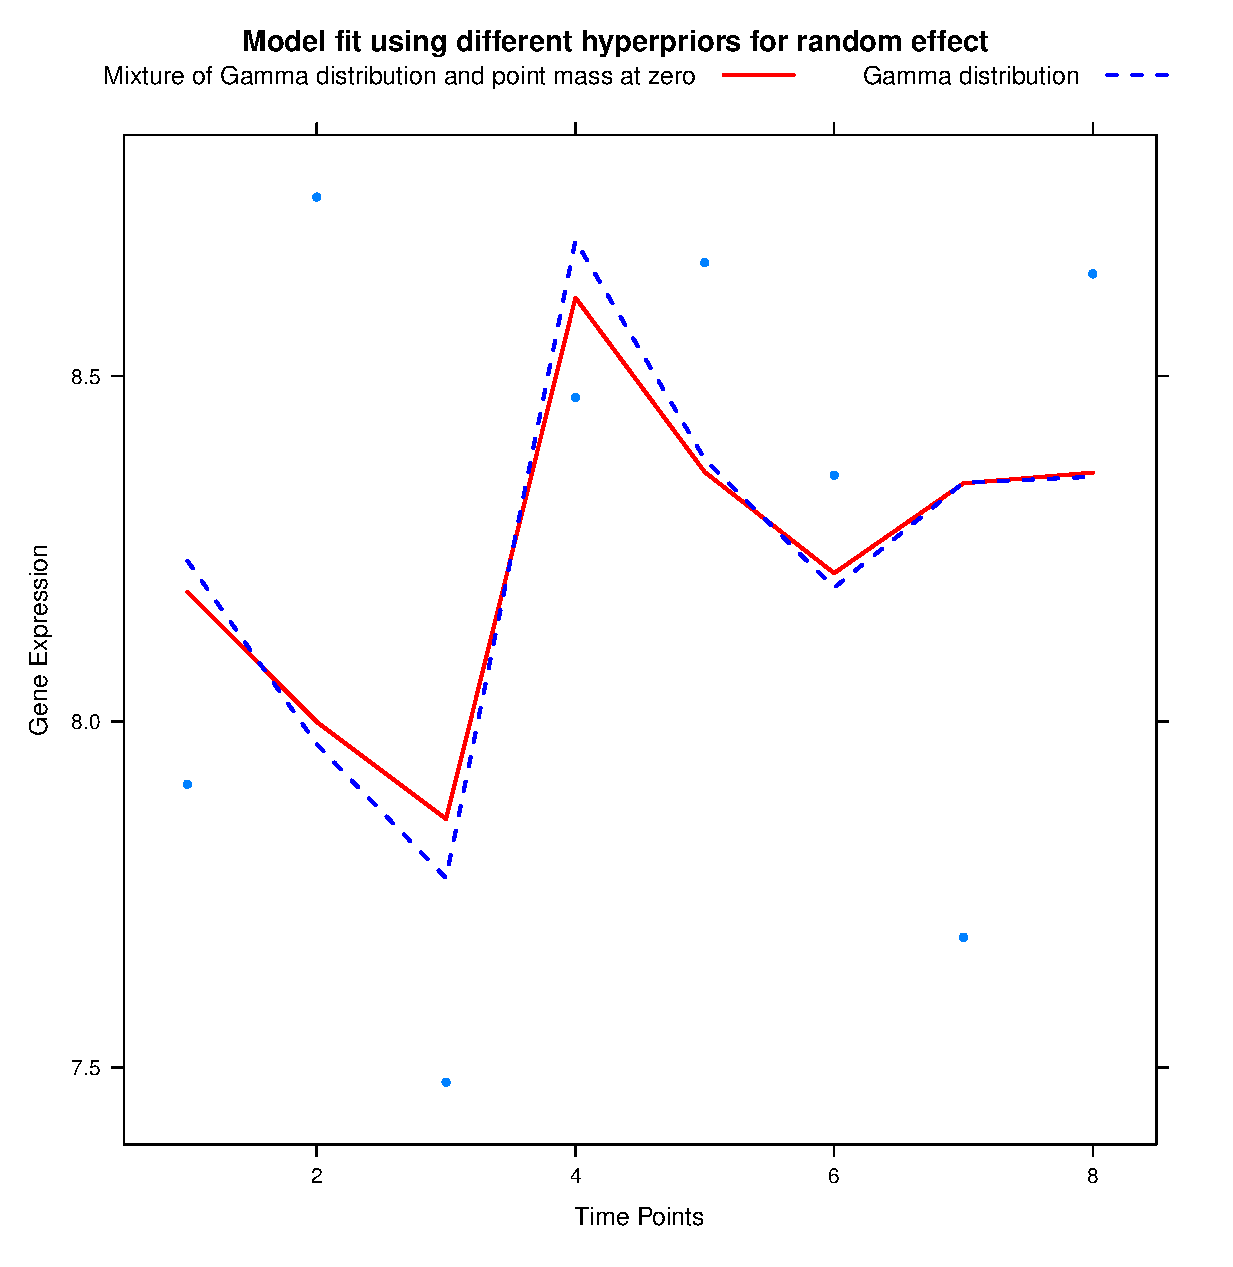
\epsfig{file=Shrinkage1.eps,width=0.45\linewidth, angle=0}
\end{tabular}
\caption{The effect of using different hyperpriors in a single cell line. Gene\\
			expression is plotted against time (single cell line only). The solid red line is the\\
 		          fit of the model with a standard hyperprior, while the dashed blue line is that of\\
 			the model with the alternative mixture hyperprior.}
\label{fig:shrinkage}
\end{figure}

\begin{figure}[h!]
\centering
\begin{tabular}{cc}
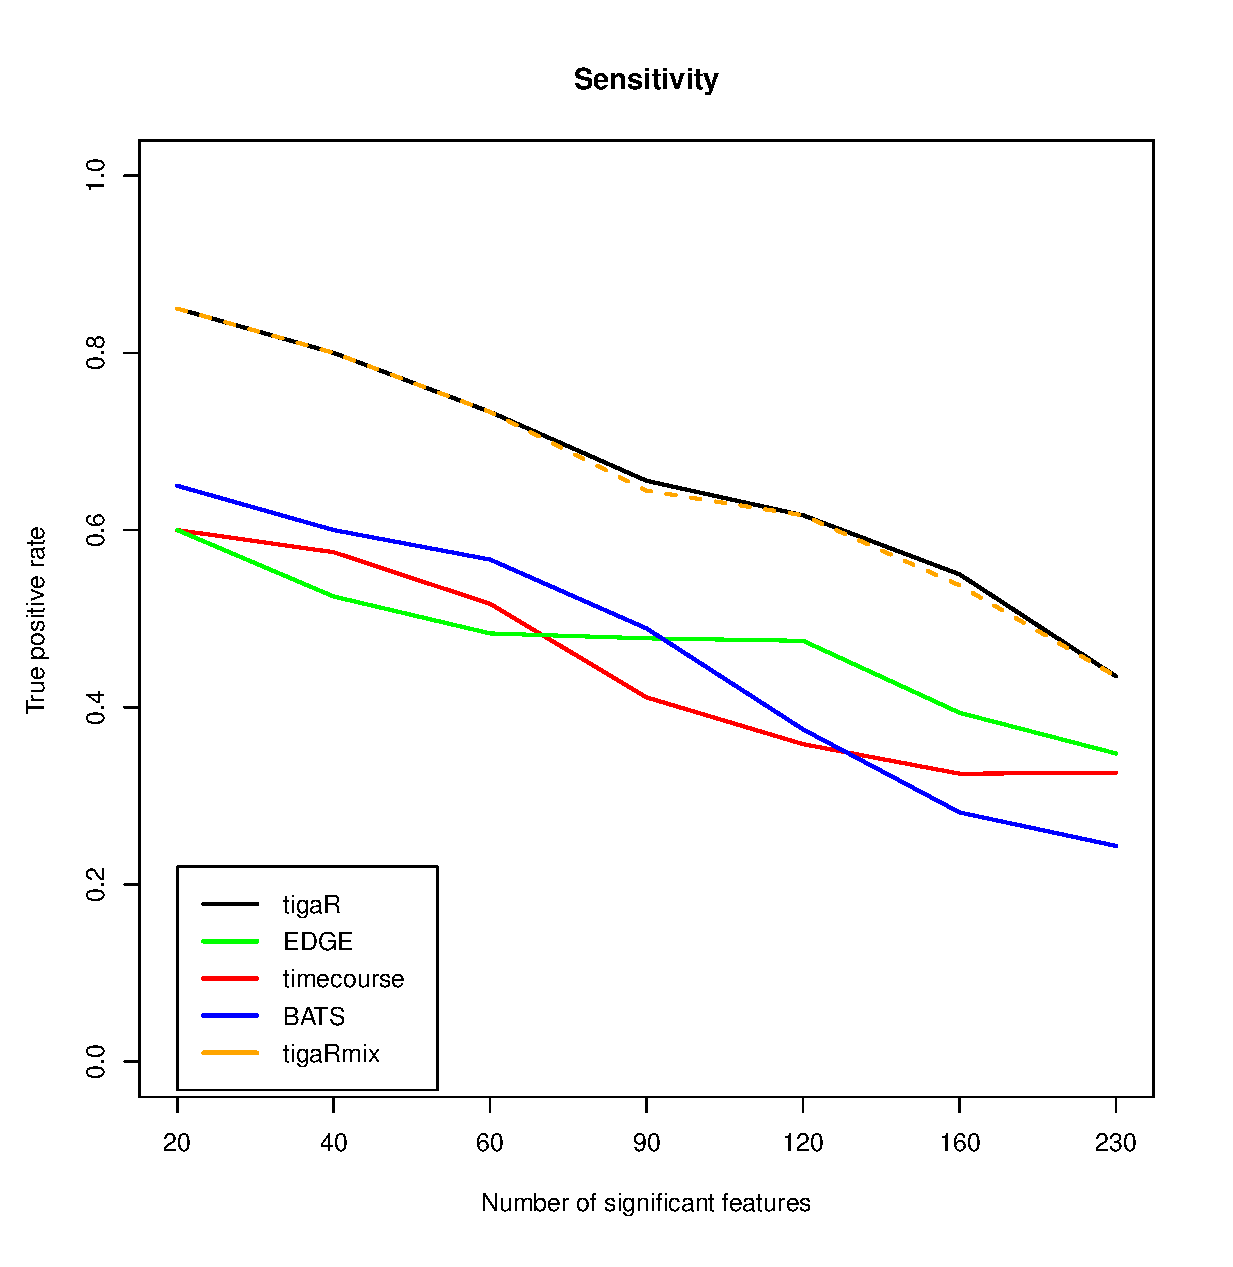
\epsfig{file=SensSpecMix1.eps,width=0.45\linewidth, angle=0}
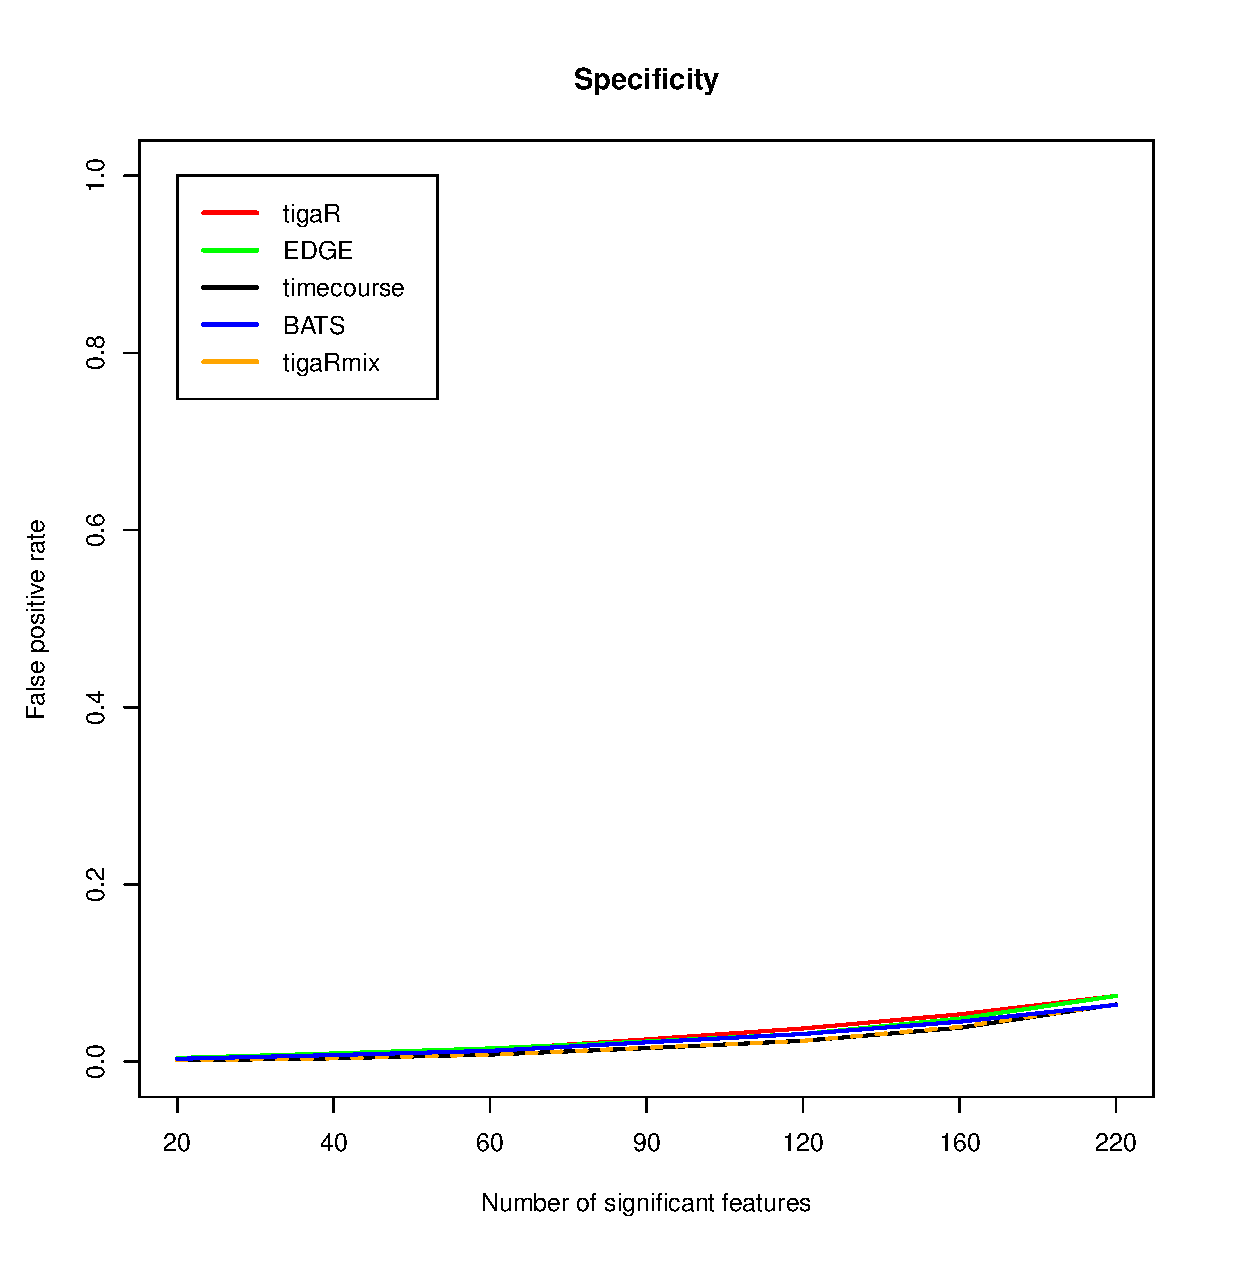
\epsfig{file=SensSpecMix2.eps,width=0.45\linewidth, angle=0}
\end{tabular}
\caption{Plots represent comparison of packages tiagR, EDGE, BATS,\\
				 timecourse and tigaR which employ hyperprior composed of Gamma and point\\
                                            mass at zero for the sensitivity and specificity on HPV-induced transformation\\
 				 data. The left panel represents the sensitivity (of each model), where the true\\
				 positive rate is plotted against the number of significant genes. The right panel\\
 				 illustrates the specificity (of each method), where the false positive rate is\\
				 plotted against the number of significant genes.}
\label{fig:mixSensSpec}
\end{figure}

\newpage

\section{Effect of a gene specific covariate on shrinkage}
DNA copy number data varies from one chromosome to another, but within a single chromosome these data exhibit genomic regions that share the same aberration patterns over the samples. We assume a common hyperprior for the gene dosage effect within and between such regions. This is justified within a region, but between regions it may be more appropriate to assume a different dirac-Gaussian hyperprior. By simulation we show that the effect of assuming a common hyperprior for all regions is not unreasonable, in the sense that it does not yield results that differ much from those obtained when employing a separate hyperprior for each region.
 
The simulation involves the data set described in Section 2.1. For 15 regions (comprising features with a common DNA copy number pattern over the samples) we estimate parameters of the gene dosage effect prior distribution with both separate Dirac-Gaussian hyperpriors and a common one, employing the procedure described in Section 1.2. First, we estimate the hyperparameters of the DNA copy number effect using a different Dirac-Gaussian hyperprior for each region.  Then, we also estimate hyperparameters of the gene dosage effect using a dirac-Gaussian hyperprior common to all regions. Figure \ref{fig:mixture} shows the histograms of the sampling distribution from the averaged (over the regions) prior and the common prior of the gene dosage effect. At first glance the histograms are similar. A better comparison is provided by the Quantile-Quantile plot (right panel of Figure \ref{fig:mixture}). The Q-Q plot reveals that these prior distributions (with separate and common Dirac-Gaussian hyperpriors) are alike around their modes, but differ somewhat in their tails. This difference in the tails will decrease as the number of regions increases. In most data sets the number of regions easily exceeds a hundred yielding a much better approximation in the tails. On the other hand, a mixture of many Gaussians with common mean but different variances may be approximated by a $t$-distribution with the degrees of freedom equal to the number of Gaussians in the mixture. Furthermore, as the degrees of freedom of a $t$-distribution  increase it approaches a Gaussian. Hence, a better approximation in the tails is expected with more regions.


\begin{figure}[h!]
\centering
\begin{tabular}{ccc}
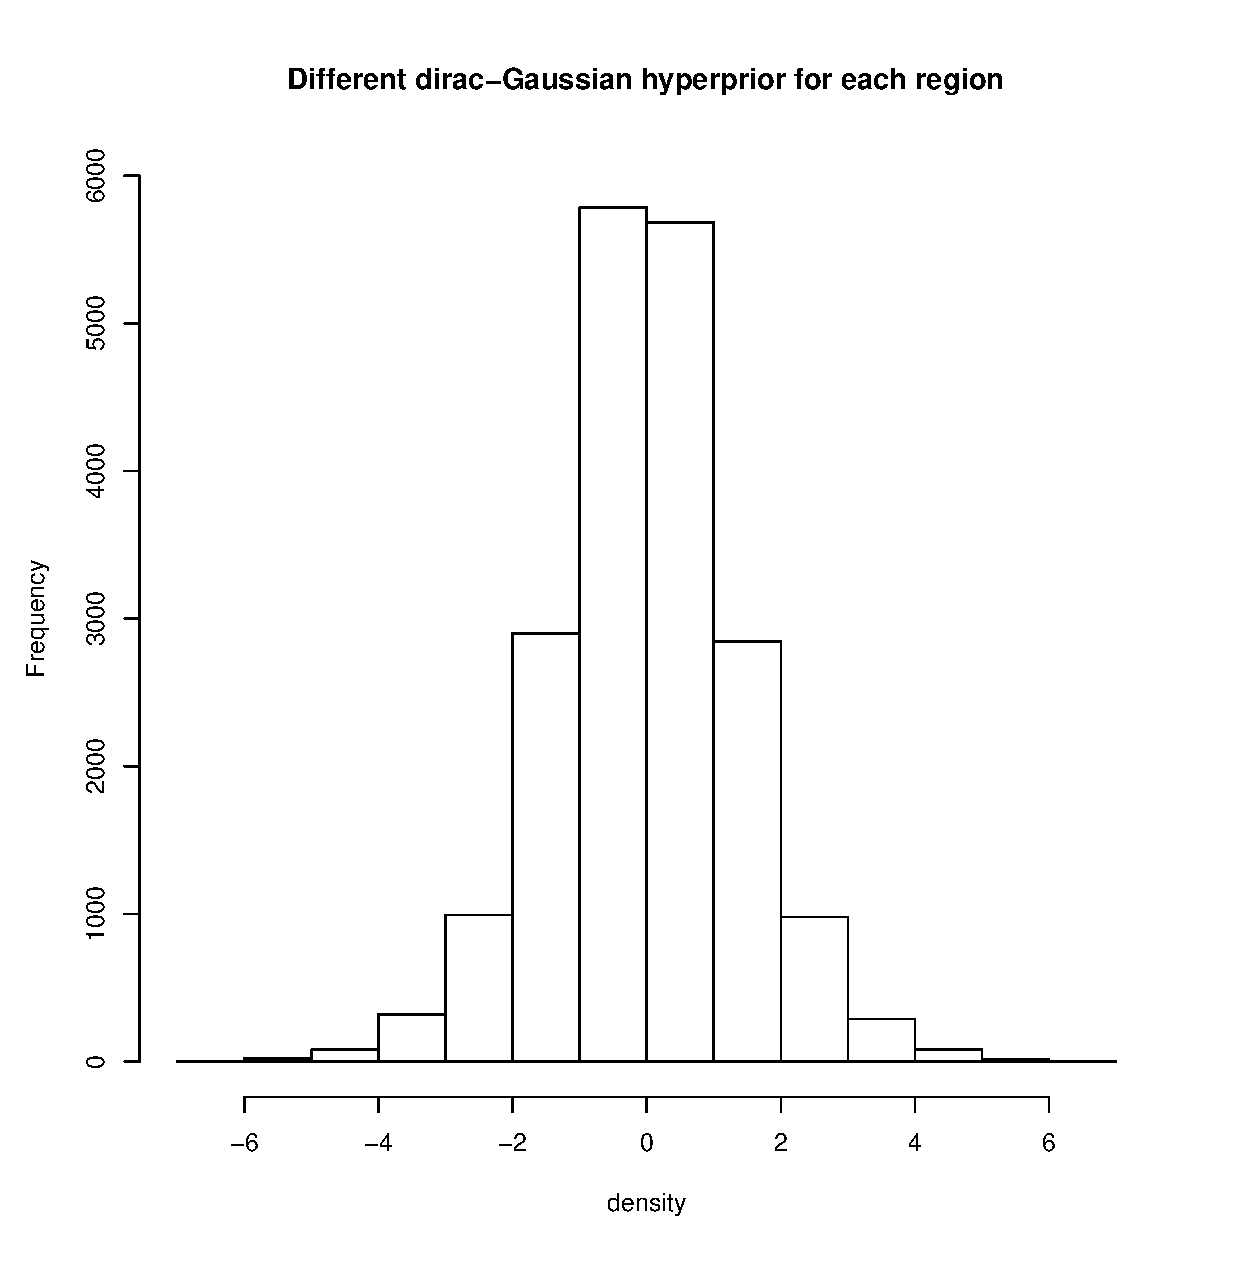
\epsfig{file=Simulation1.eps,width=0.32\linewidth, angle=0}
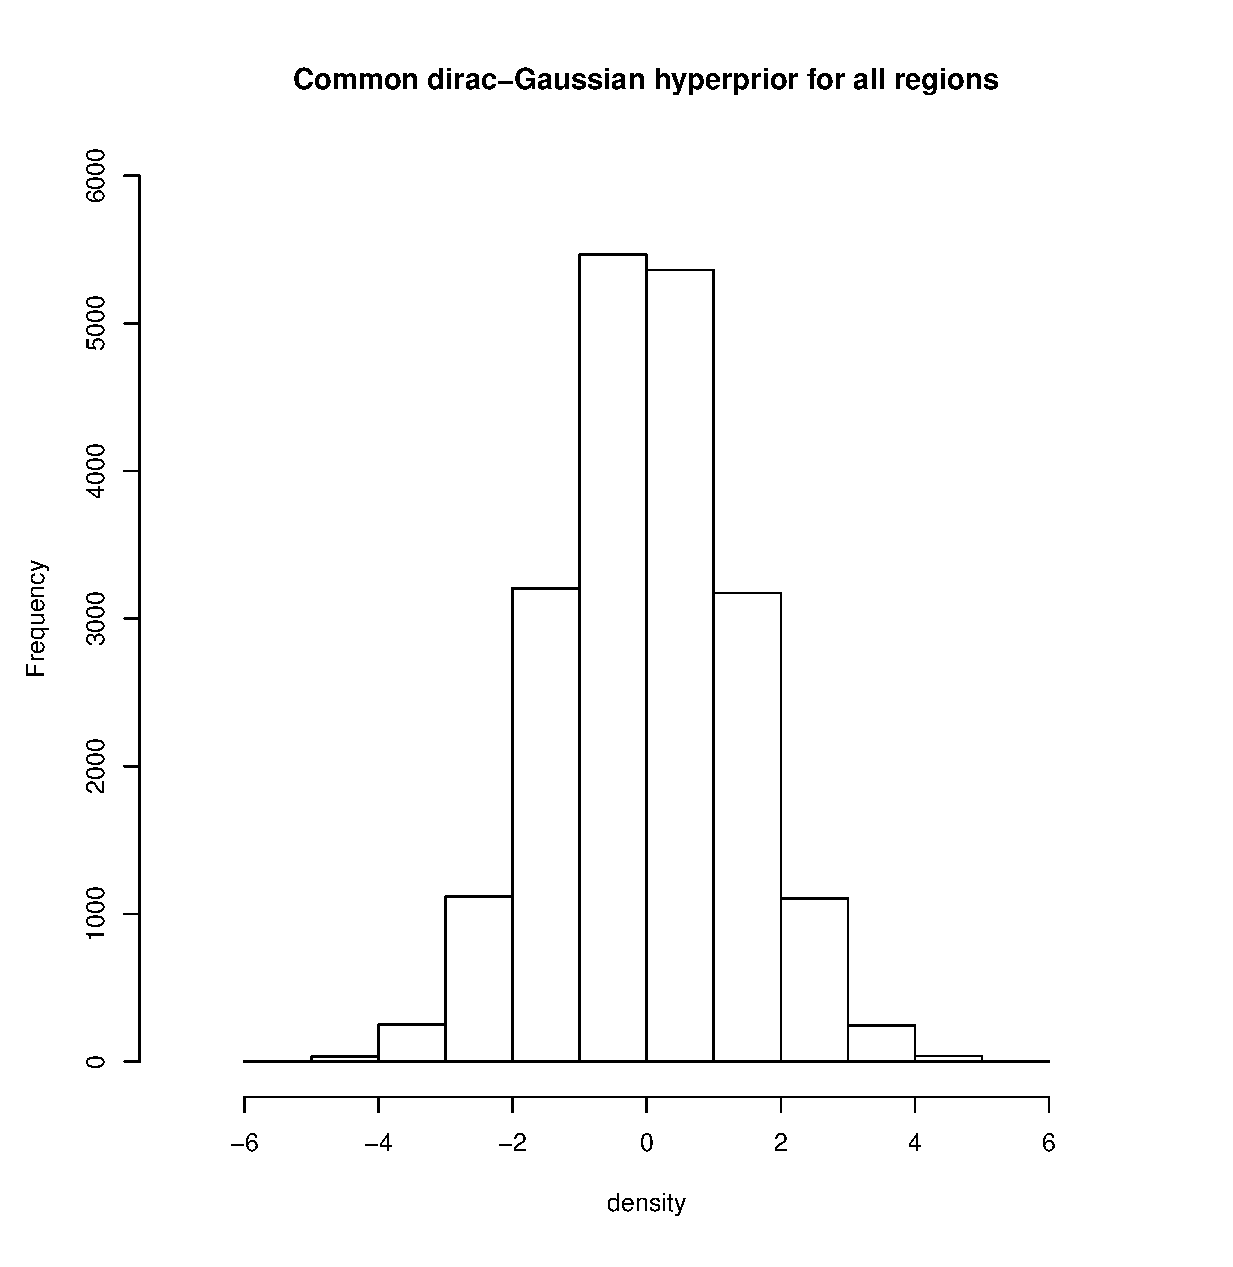
\epsfig{file=Simulation2.eps,width=0.32\linewidth, angle=0}
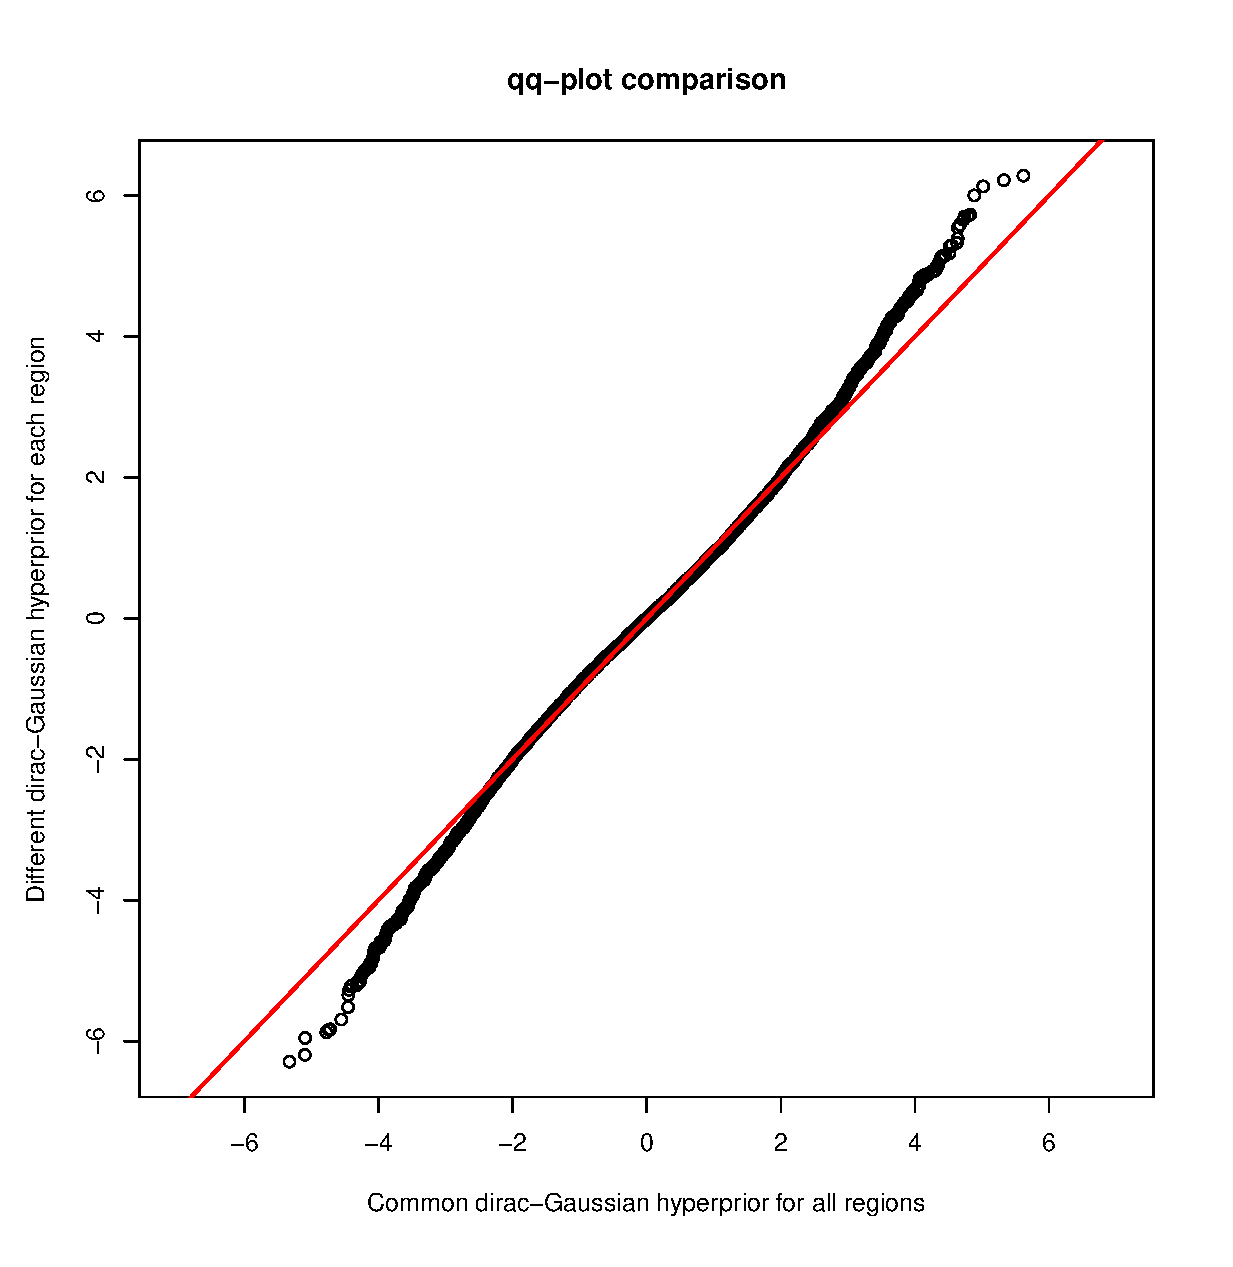
\epsfig{file=Simulation3.eps,width=0.32\linewidth, angle=0}
\end{tabular}
\caption{Comparison of common and separate Dirac-Gaussian hyperpriors. The\\
 				 left panel depicts the prior distribution of the gene dosage effect using a\\
				 common Dirac-Gaussian hyperpriors for all regions. The middle panel \\
				 represents the prior distribution for different Dirac-Gaussian hyperpriors per\\
				 region. The right panel compares these distributions using a Q-Q plot.}
\label{fig:mixture}
\end{figure}



\newpage
\section{Degree of freedom estimation for penalized splines}
Within the context of generalized linear mixed models the effective degrees of freedom are (usually) defined by the trace of the hat matrix. The fit of the mixed Model (2) per gene $j$ is obtained by $\hat{\mathbf{Y}}_{j}=\mathbf{H}_{\lambda,j}\mathbf{Y}_{j}$, where $\mathbf{H}_{\lambda,j}$ is the hat matrix, which projects the data onto the space spanned by the design matrix. The matrix $\mathbf{Y}_{*,j,*}$ is transformed into a vector by the $\mbox{vec}$-operator: $\mathbf{Y}_j=\mbox{vec}(\mathbf{Y}_{*,j,*})$, where the measurements of gene $j$ are first ordered by cell lines $i$ and within a cell line by time. The hat matrix for Model (2) is defined using smoothing parameter $\lambda= \sigma_{\gamma,j}^2 / \sigma_{\varepsilon,j}^2$, which controls the smoothness of the fit. Let  $\mathbf{C}_j$ be the joint design matrix comprising covariate information for both the fixed and random effects. The hat matrix is then:
\[
\mathbf{H}_{\lambda,j}=\mathbf{C}_j\left(\mathbf{C}_j^\mathrm{T}\mathbf{C}_j+\lambda \mathbf{I}\right)^{-1}\mathbf{C}_j^\mathrm{T}.
\]
We exemplify the use of the matrix $\mathbf{C}_j$. Consider the data set from Section 2.1 using a model with a common spline. Then, $\mathbf{C}_{j}= [\mathbf{W}_{i,t}|\tilde{\mathbf{Z}}_t ]$, where $\mathbf{W}_{i,t}$ is a matrix with cell line and DNA copy number covariate information, while  $\tilde{\mathbf{Z}}_t$ contains that for the random (time) effect. Matrix $C_j$ has dimensions $32\times7$, where 32 corresponds to the number of observations on gene $j$, while 7 represents the number of covariates: four cell line effects, one gene dosage effect, and two for the spline (a common spline with two knots). The rows of $\mathbf{C}_j$ are ordered as those of $\mathbf{Y}_j$.


Generalizing the definition of degrees of freedom, it is defined as the trace of the hat matrix: $\mbox{df} =  \mbox{tr}(\mathbf{H}_{\lambda,j})$.
This is thus the degree of freedom of mixed Model (2), depending on the smoothing parameter $\lambda$. It can be interpreted as the number of fitted parameters. Thus, $\mbox{df}$ indicates the `amount of fitting' done by $\mathbf{H}_{\lambda,j}$, which is strictly monotone in $\lambda$.


\newpage
\section{Parameter estimation using the spatial prior}
In this section we present how parameters of Model (2) are re-estimated when imposing a spatial prior on the gene dosage effect. First, all hyperparameters of Model (2) are estimated univariate as described in Section 1.2. Then, hyperparameter $\rho$ (of the spatial prior) is estimated by regressing $\beta_j$ on $\beta_{j-1}$ (justified by the assumption that $\beta_j$ follows a first-order autoregressive process). Combining the univariate estimated hyperparameters $\sigma_{j-1}^2, \sigma_{j}^2, \sigma_{j+1}^2$ with the estimated spatial hyperprior parameter $\rho$, yields the covariance matrix of the spatial hyperprior of a contiguous triplet. With this estimated spatial prior and the other (univariate) priors at hand, model parameters are re-estimated trivariately (per triplet of contiguous genes). Due to the fact that INLA does not allow to estimate a trivariate model with an AR(1) covariance structure on a fixed effect, estimators of model parameters are derived analytically.


Analytical estimators are derived separately for fixed and random effects. For convenience of notation we write $\mathbf{W}_{i,j}$, the joint design matrix of the cell line and DNA copy number information, and $\boldsymbol{\theta}_j=(\boldsymbol{\alpha}_{i,j}, \beta_j)$, the vector of corresponding parameters. Further, the prior distributions for fixed and random effects can be written as $\boldsymbol{\theta}_j|\sigma_{\theta,j}^2\sim \mathcal{N}(\mathbf{0},\sigma_{\theta,j}^2 \mathbf{\Sigma})$ and$\boldsymbol{\gamma}_j|\sigma_{\gamma,j}^2\sim \mathcal{N}(\mathbf{0},\sigma_{\gamma,j}^2 \mathbf{\Psi})$, for appropriate covariance matrices  $\mathbf{\Sigma}$ and $\mathbf{\Psi}$. The part of covariance matrix $\mathbf{\Sigma}$ corresponding to parameters $\beta_j$ incorporates the AR(1) correlation structure.
 
 
From \cite{Sorensen2002} we obtain the estimator of the fixed effect in a trivariate linear mixed model, given the hyperparameters:
\begin{eqnarray*}
\boldsymbol{\hat{\theta}}_j & = & \left( \mathbf{W}_{i,j}^\mathrm{T}\mathbf{V}_j^{-1}\mathbf{W}_{i,j} + \mathbf{\Sigma}^{-1}\frac{\sigma_{\varepsilon,j}^2}{\sigma_{\theta,j}^2} \right)^{-1} \mathbf{W}_{i,j}^\mathrm{T}\mathbf{V}_j^{-1}\mathbf{Y}_{*,j,*},
\end{eqnarray*}
where
\begin{eqnarray*}
\mathbf{V}_j^{-1} & = & \left( \tilde{\mathbf{Z}}_t\mathbf{\Psi} \tilde{\mathbf{Z}}_t^\mathrm{T}\frac{\sigma_{\varepsilon,j}^2}{\sigma_{\gamma,j}^2}+\mathbf{I} \right)^{-1}.
\end{eqnarray*}
Using $\boldsymbol{\hat{\theta}}$ and previously estimated hyperparameters, the random effect estimator from a trivariate linear mixed model is:
\begin{eqnarray*}
\boldsymbol{\hat{\gamma}}_j(\boldsymbol{\hat{\theta}}_j) & = & \left( \tilde{\mathbf{Z}}_t^\mathrm{T}\tilde{\mathbf{Z}}_t + \mathbf{\Psi}^{-1}\frac{\sigma_{\varepsilon,j}^2}{\sigma_{\gamma,j}^2}\right)^{-1} \tilde{\mathbf{Z}}_t^\mathrm{T}
\left( \mathbf{Y}_{*,j,*}-\mathbf{W}_{i,j}\boldsymbol{\hat{\theta}}_j \right).
\end{eqnarray*}
Full derivation of these estimators can be found in Chapter 6 of \cite{Sorensen2002}. 

With these analytic estimators we obtain the trivariate fit of the model. From this trivariate fit, only the parameter estimate of the middle gene in the triplet is preserved and considered its final parameter estimate. Sliding the triplet window over the genome yields final parameter estimates for each gene.




\newpage
\section{Optimal number of knots for penalized splines}
DIC is a measure that combines model fit with model complexity (the latter is represented by the number of effective parameters) (\cite{Spiegelhalter2002}).
When denoting by $\boldsymbol{\theta}_j$ the vector containing all parameters of Model (2), then the goodness-of-fit (for gene $j$) may measured by the deviance $D(\boldsymbol{\theta}_j)=-2\log[L(Y_{*,j,*}|\boldsymbol{\theta}_j)]$. Write $D(\bar{\boldsymbol{\theta}}_j)=D(E_{\boldsymbol{\theta}_j|Y_{*,j,*}}[\boldsymbol{\theta}_j])$ for the deviance of the posterior mean, where $\bar{\boldsymbol{\theta}}_j$ is the expectation of $\boldsymbol{\theta}_j$ and $\bar{D}(\boldsymbol{\theta}_j)=E_{\boldsymbol{\theta}_j|Y_{*,j,*}}[D(\boldsymbol{\theta}_j)]$ for the posterior mean of the deviance. The effective number of parameters $p_{D,j}$  is then calculated per gene as:
\[
p_{D,j} \, \, \, = \, \, \, \bar{D}(\boldsymbol{\theta}_j)-D(\boldsymbol{\bar{\theta}}_j),
\]
The effective number of parameters $p_{D,j}$ may also be defined directly through the effective degrees of freedom. For the normal hierarchical model, $p_{D,j}=\mbox{tr}(\mathbf{H}_{\lambda,j})$, with $\mathbf{H}_{\lambda,j}$ the hat matrix (\cite{Spiegelhalter2002}). The DIC is now defined as:
\[
DIC_j\, \, \, = \, \, \, D(\bar{\boldsymbol{\theta}}_j) + 2p_{D,j} \, \, \, = \, \, \, \bar{D}+p_{Dj}.
\]
\mbox{ }
\\
To decide on the optimal number of knots, we determine the DIC per gene for different numbers of knots $k=2,\ldots,5$. The value of $k$ with the smallest DIC represents the model which is the best supported by the data (for that particular gene). The optimal number of knots for the whole data set (i.e. all genes) is that $k$ which is the most frequent optimal $k$ over the genes. For the data set from Section 2.1, Figure \ref{fig:DIC} indicates that $k=2$ is the optimal number of knots.

\begin{figure}[h!]
\centering
\begin{tabular}{c}
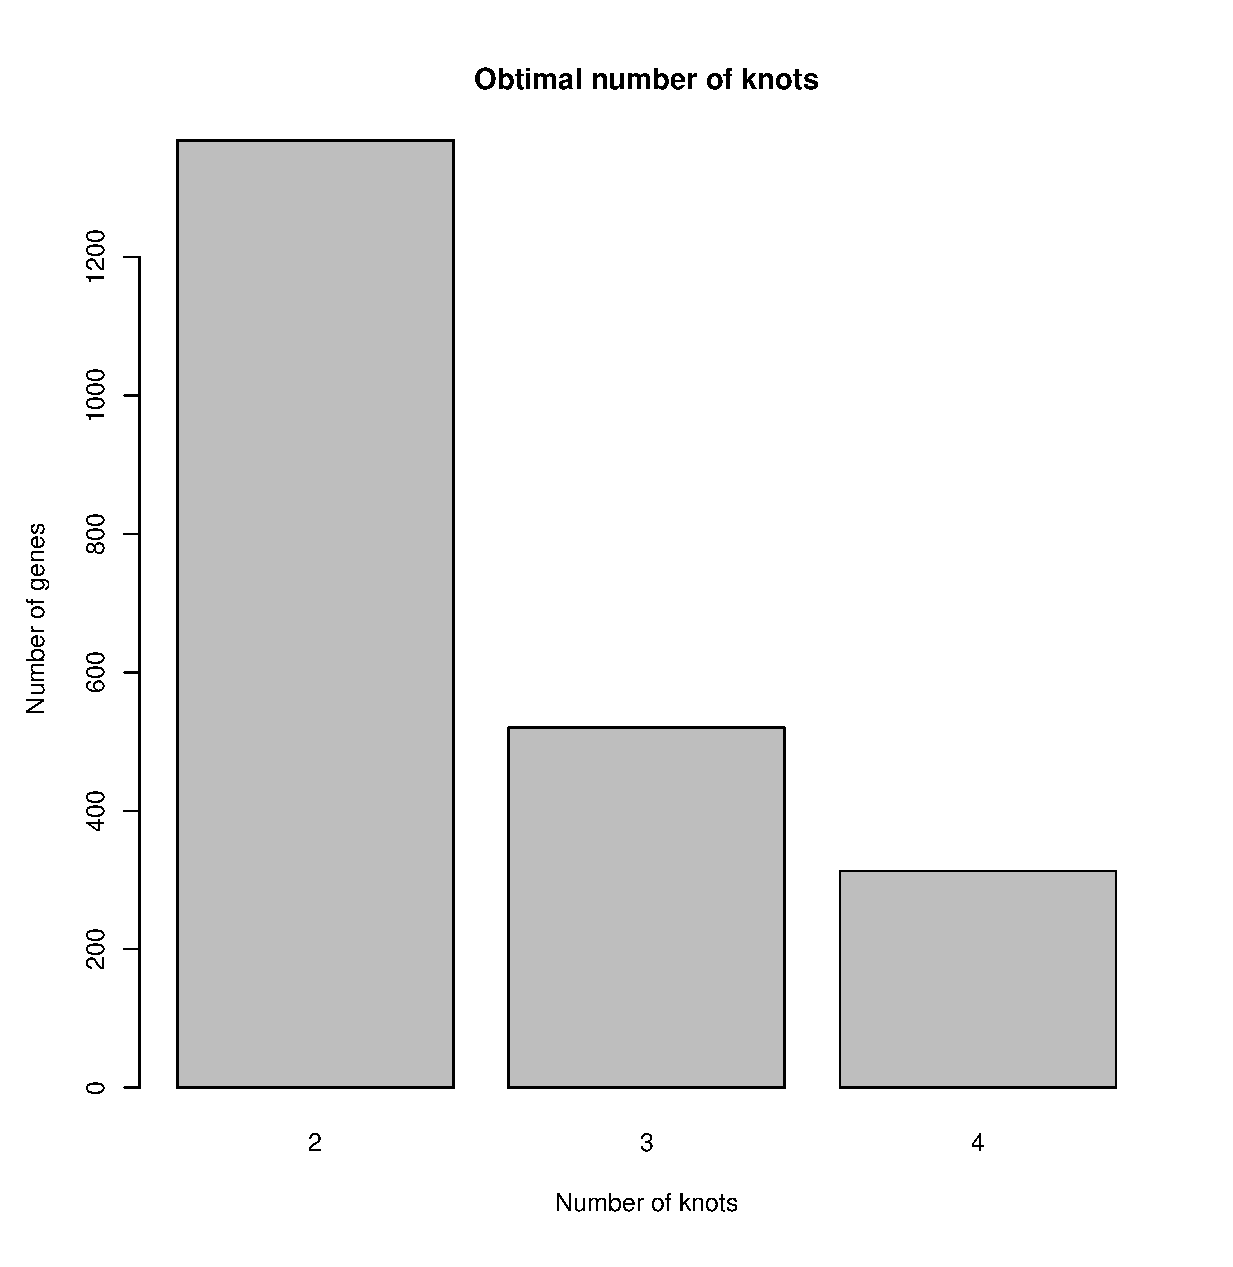
\epsfig{file=NumKnots.eps,width=0.45\linewidth, angle=0}
\end{tabular}
\caption{The bar plot illustrates the frequency of genes where the number of \\
 				 knots $k$ is identified with the smallest DIC.}
\label{fig:DIC}
\end{figure}


\newpage
\section{Comparison using the data set from the EDGE package}
The proposed method for temporal differential expression was developed with the data set from Section 2.1 in mind. This may accidentally favor our method in the comparison with its competitors EDGE, timecourse, BATS and the reference (univariate fitted) method. Therefore the comparison is repeated using the data set from EDGE-package (\cite{Storey2005}), thus possibly favoring the EDGE. Again sensitivity, specificity and reproducibility are compared among packages EDGE, timecourse, tigaR, BATS and the reference method. Figure \ref{fig:SensSpec} shows the number of true and false positive rates of the four methods. Qualitatively the same picture emerges as from the comparison using the data from Section 2.1. Similarly, when comparing the reproducibility of the methods (confer Figure \ref{fig:reprod}), again tigaR and BATS outperform  timecourse and EDGE.


\begin{figure}[h!]
\centering
\begin{tabular}{cc}
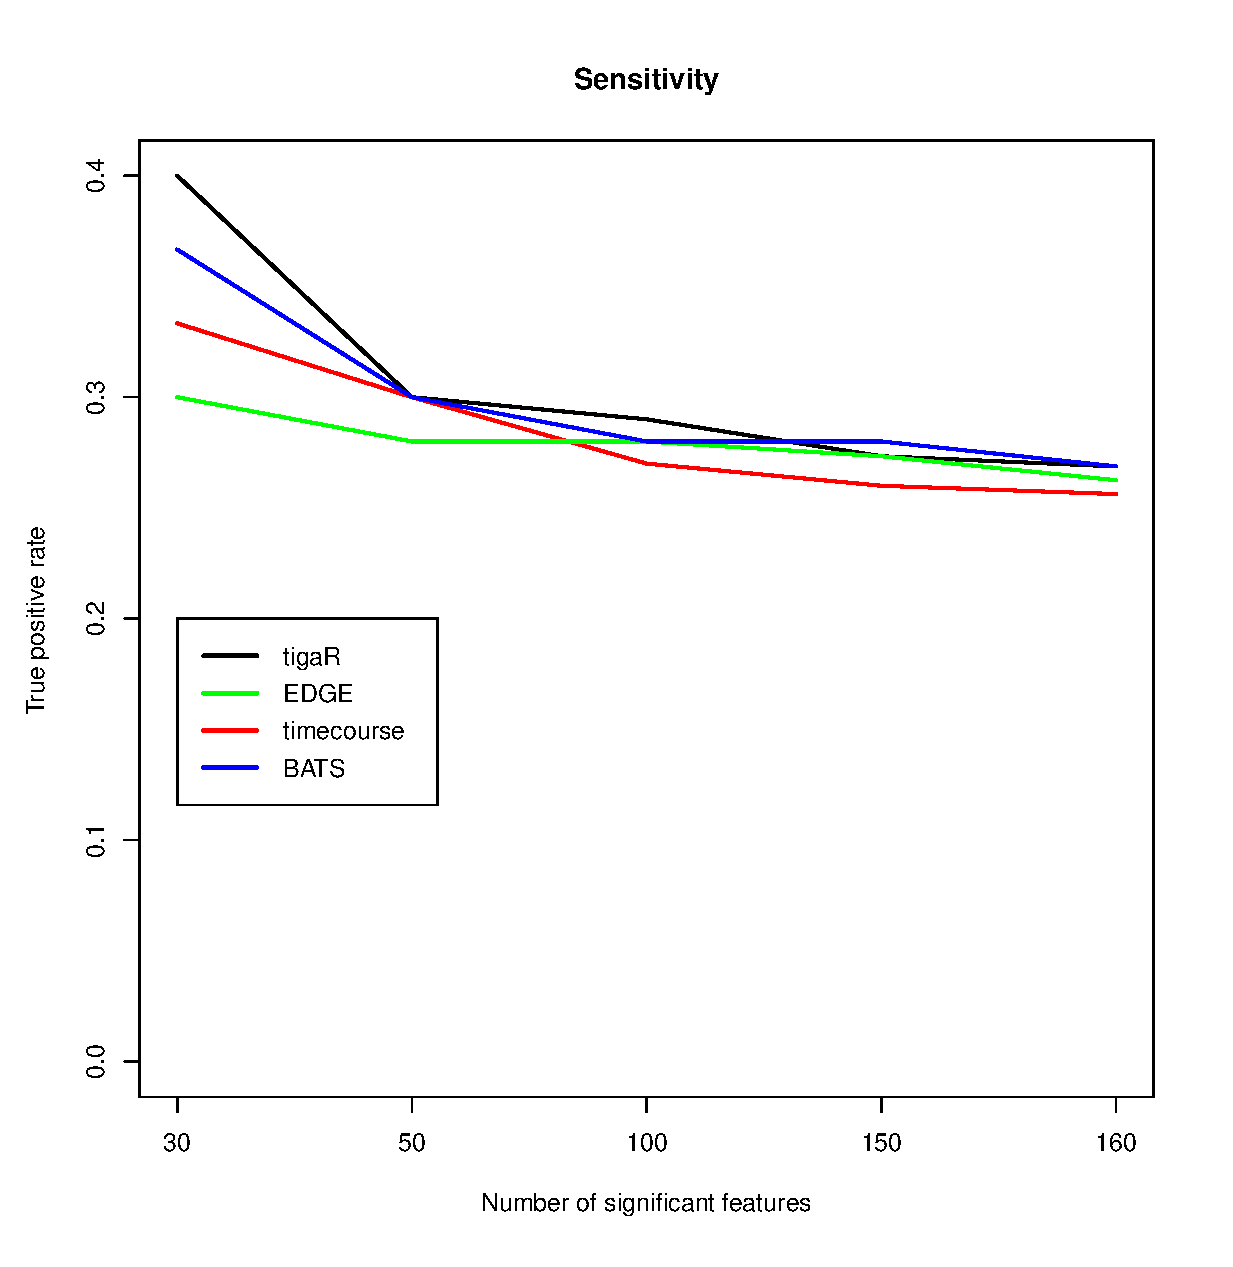
\epsfig{file=SensSpecEdge1.eps,width=0.45\linewidth, angle=0}
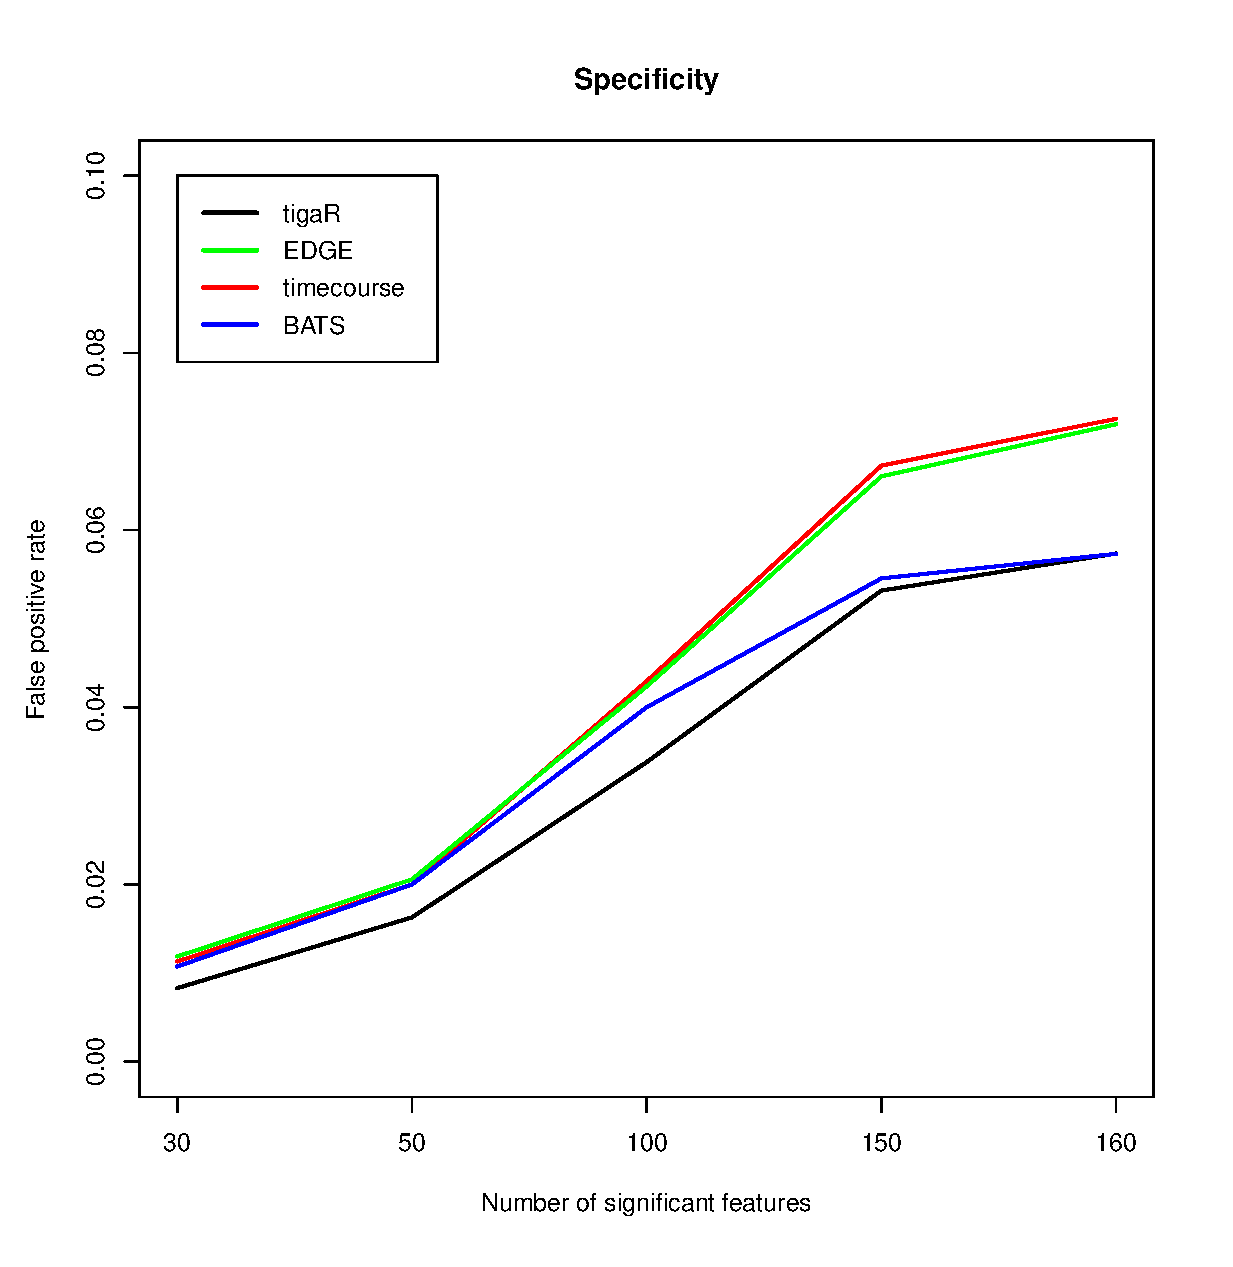
\epsfig{file=SensSpecEdge2.eps,width=0.45\linewidth, angle=0}
\end{tabular}
\caption{Plots represent comparison of tigaR, EDGE, timecourse and BATS\\
				 package for the sensitivity and specificity on the data set from the EDGE-\\
				 package. The left panel represents the sensitivity (of each model), where the\\
				 true positive rate is plotted against the number of significant genes. The right\\
				 panel illustrates the specificity (of each method), where the false positive rate is\\
				 plotted against the number of significant genes.}
\label{fig:SensSpec}
\end{figure}

\newpage

\begin{figure}[h!]
\centering
\begin{tabular}{c}
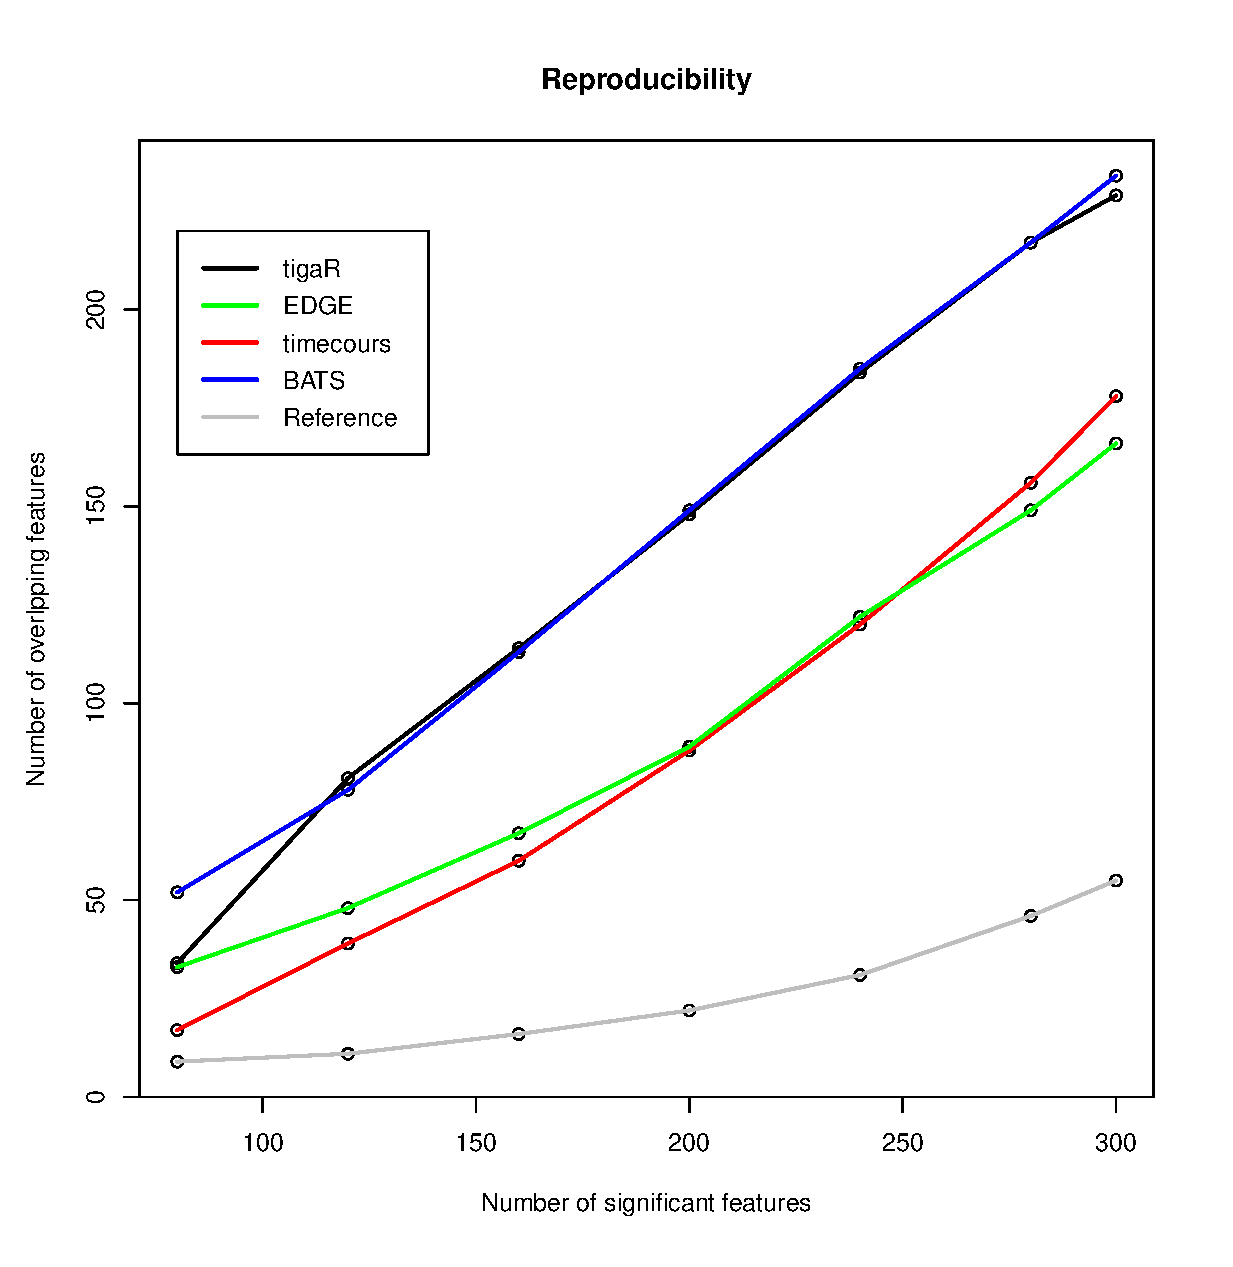
\epsfig{file=ReproduciabilityEdge1.eps,width=0.45\linewidth, angle=0}
\end{tabular}
\caption{The plot illustrates the comparison of the reproducibility between\\
				 tigaR, EDGE, timecourse, BATS and reference model. The number of\\
				 significant genes is plotted against number of overlapping genes identified\\
				 between two groups.}
\label{fig:reprod}
\end{figure}




\newpage
\section{Additional plots}
In the main manuscript Figure 2, Figure 6 and Figure 7 show only a single cell line. This is done for reasons of clarity: to make a certain effect more visible. Here, in Figure \ref{fig:spatialFit}, Figure \ref{fig:SLC25A36} and Figure \ref{fig:priors} these effects are shown in all four cell lines.

Additionally, a Venn diagram (Figure \ref{fig:VennDiagram}) is presented. It illustrates the various intersections of the sets of features exhibiting temporal differential expression as declared by tigaR, EDGE, timecourse and BATS. The timecourse packages only provides a rank-ordered list of genes. For the comparison the top genes from this list are selected, their number being equal to the number of features selected by tigaR (with a common spline).

\begin{figure}[h!]
\centering
\begin{tabular}{c}
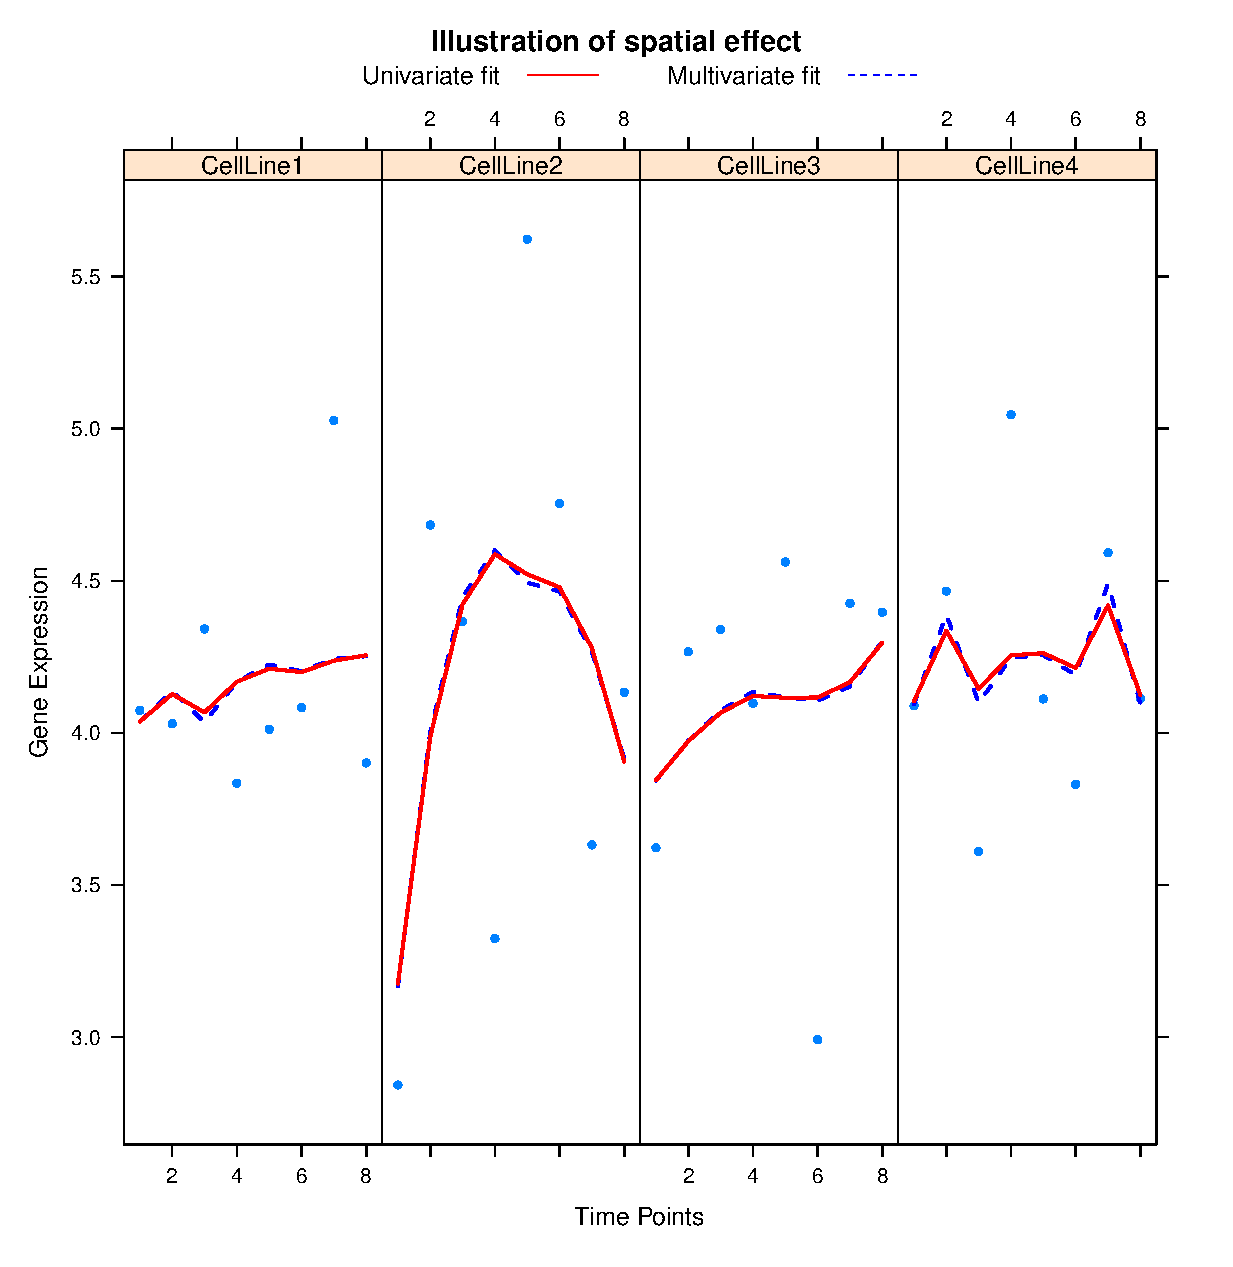
\epsfig{file=SpatialEffect_full-new.eps,width=0.45\linewidth, angle=0}
\end{tabular}
\caption{Illustration of the effect of the spatial prior of one gene in four cell\\
 				 lines. Gene expression is plotted against time (in four cell lines). The lines\\
         represent the univariate (red, solid line) and multivariate fit (blue, dashed 		  				 line).}
\label{fig:spatialFit}
\end{figure}

\begin{figure}[h!]
\centering
\begin{tabular}{c}
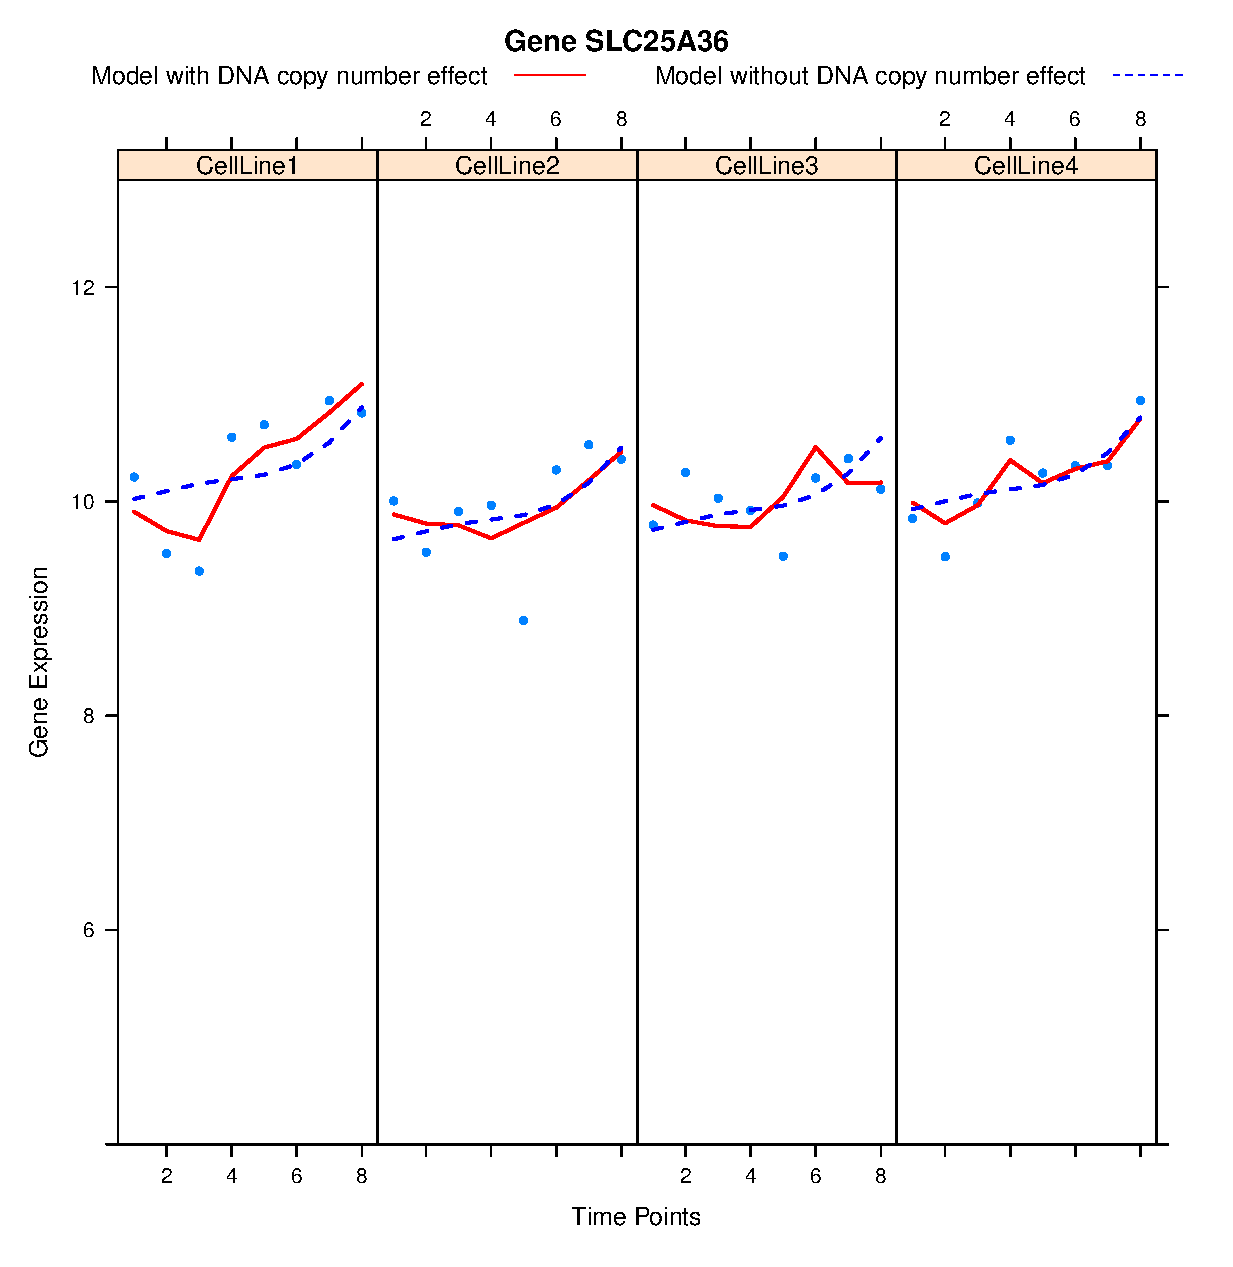
\epsfig{file=SLC25A36_full-new.eps,width=0.45\linewidth, angle=0}
\end{tabular}
\caption{Dots represent expression levels of gene SLC25A36 plotted against\\
 				 time in four cell lines. The solid (red) line represents the full model while the\\
 				 dashed (blue) line illustrates the fit of the model without copy number effect.}
\label{fig:SLC25A36}
\end{figure}

\begin{figure}[h!]
\centering
\begin{tabular}{c}
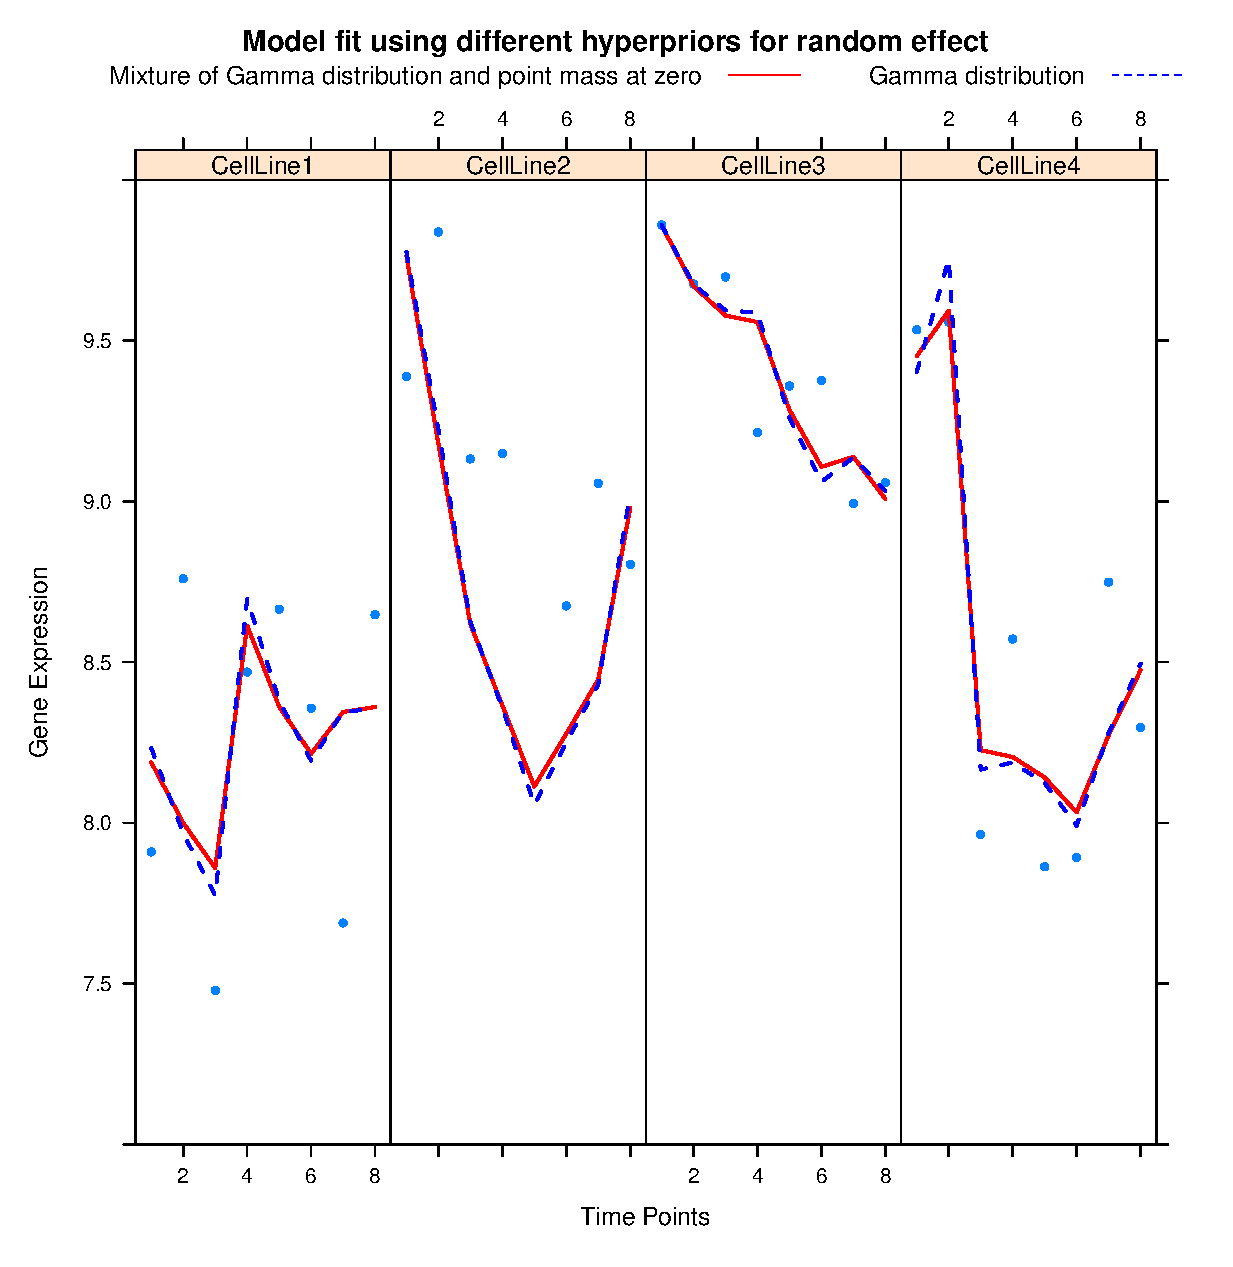
\epsfig{file=Shrinkage_full1.eps,width=0.45\linewidth, angle=0}
\end{tabular}
\caption{Effect of using different priors in four cell lines. Gene expression is\\
      plotted against time (in four cell lines). The solid red line is the fit of the model\\
 			with a standard prior, while the dashed blue line is that of the model with an\\ 
			alternative prior.}
\label{fig:priors}
\end{figure}

\begin{figure}[h!]
\centering
\begin{tabular}{c}
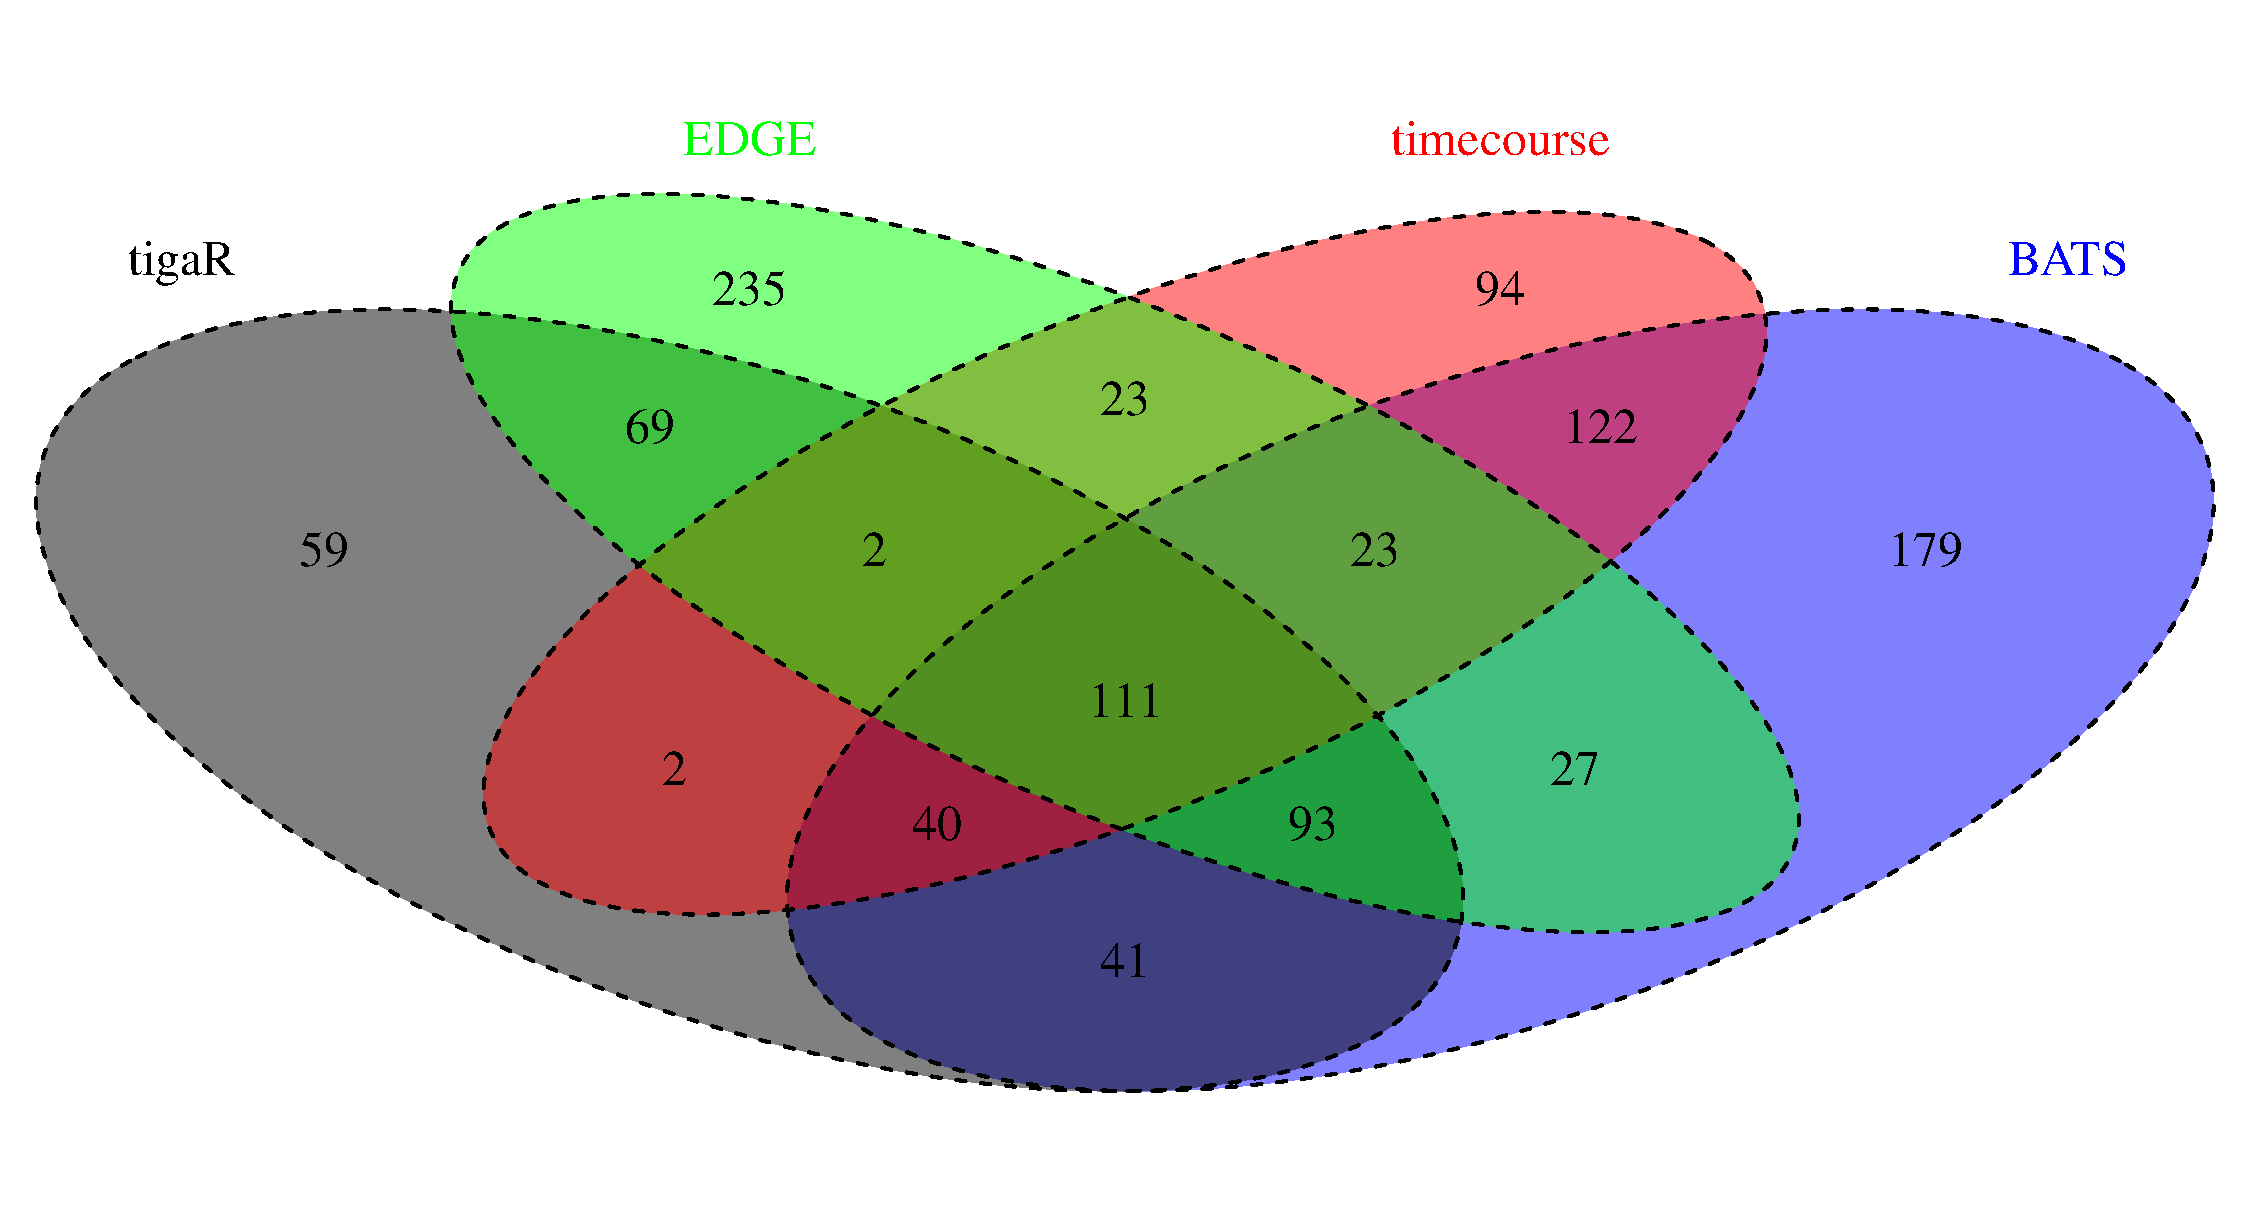
\epsfig{file=Venn.pdf,width=0.45\linewidth, angle=0}
\end{tabular}
\caption{ Venn diagram of methods tigaR, EDGE, timecourse and BATS.}
\label{fig:VennDiagram}
\end{figure}


\chapter{Ridge estimation of the VAR(1) model and its time series chain graph from multivariate time-course omics data \\ {\footnotesize (\textit{Miok, V., Wilting, S. M. and van Wieringen, W. N., Biometrical Journal (2017), 59(1), 172-191})}}
\label{ch3:ragt2ridges}
\chaptermark{Ridge estimation of the VAR(1) model}
\label{chapter:Estimating entropy loss in Gaussian graphical models}
\graphicspath{{Chapter3/Figs/}{Chapter3/Figs/PDF/}{Chapter3/Figs/}}%


\newpage
\section{Pseudo-code of ridge ML estimation}
\begin{minipage}[h]{\textwidth}
\begin{center}
\fbox{\parbox{13cm}{
\vspace{0.2cm}
{\it Box 1:} Ridge ML estimation of the parameters of the VAR(1) model. \vspace{0.2cm}
\\
\textbf{Initiate}
\newline
Obtain an initial estimate $\hat{\mathbf{A}}^{(0)}(\lambda_a)$ of $\mathbf{A}$ from the ridge OLS estimator.
\vspace{0.2cm}
\newline
\textbf{Iterate}
\newline
For $k=1, \ldots, k_{\mbox{{\tiny max}}}$ iterate the following steps:
% \\
\begin{compactitem}
\item[1)] Use the latest estimate of $\mathbf{A}$, $\hat{\mathbf{A}}^{(k-1)}(\lambda_a)$, to calculate the sample error covariance matrix  $\mathbf{S}_{\varepsilon}^{(k)}$. Given $\mathbf{S}_{\varepsilon}^{(k)}$, the ridge ML precision estimator yields the updated estimate of $\mathbf{\Omega}_{\varepsilon}$,  $\hat{\mathbf{\Omega}}_{\varepsilon}^{(k)} (\lambda_{\omega})$.

\item[2)] Get $\hat{\mathbf{A}}^{(k)}(\lambda_a)$ from
the ridge ML estimator of $\mathbf{A}$ with $\hat{\mathbf{\Omega}}_{\varepsilon}^{(k)} (\lambda_{\omega})$ substituted for $\mathbf{\Omega}_{\varepsilon}$.
\end{compactitem}
\mbox{ }
\vspace{-0.2cm}
\newline
\textbf{Terminate}
\newline
Iterate the previous step, until convergence.
\vspace{0.2cm}
}
}
\end{center}
\end{minipage}
\mbox{ }

\newpage
\section{Comparison of computation time}
\begin{figure}[h!]
\centering
\begin{tabular}{ll}
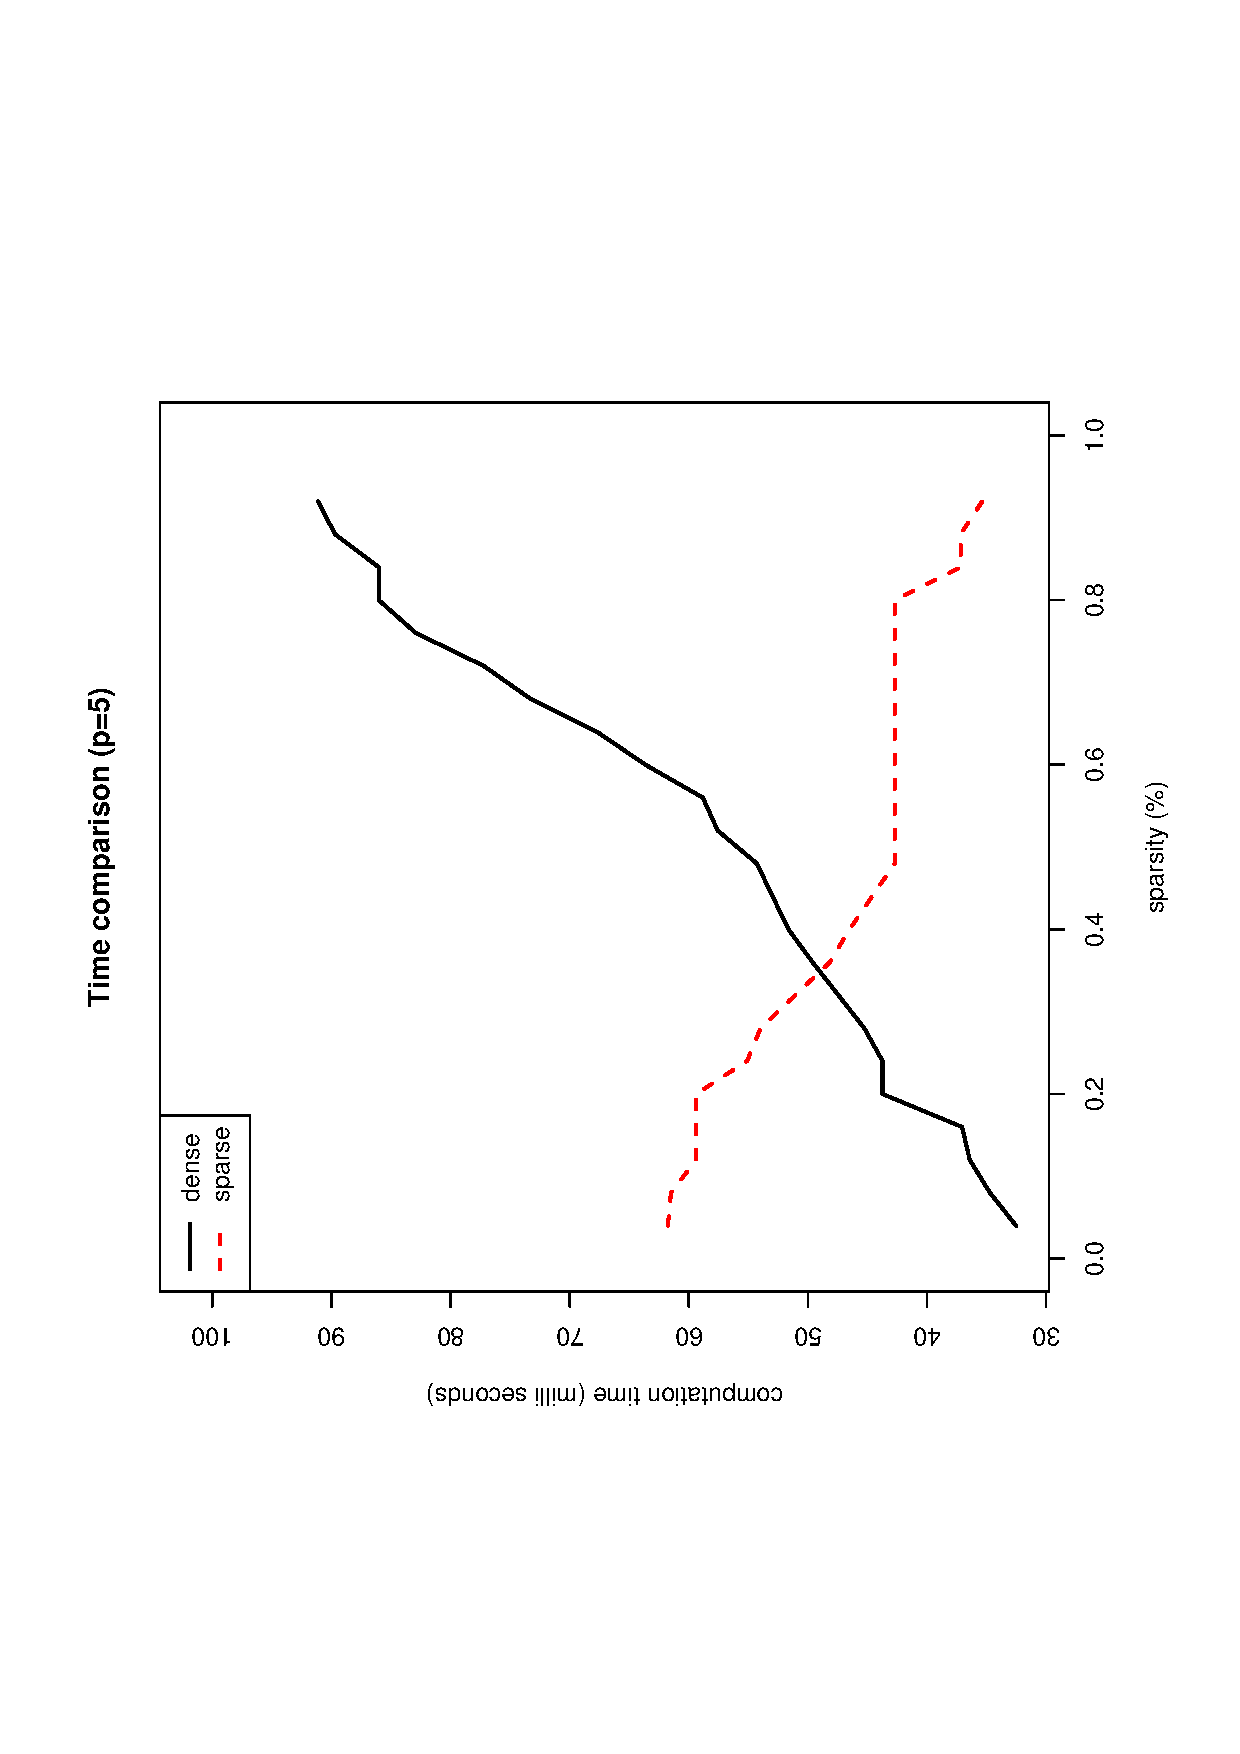
\includegraphics[scale=0.28,angle=270]{timeComparison_p05.pdf} &
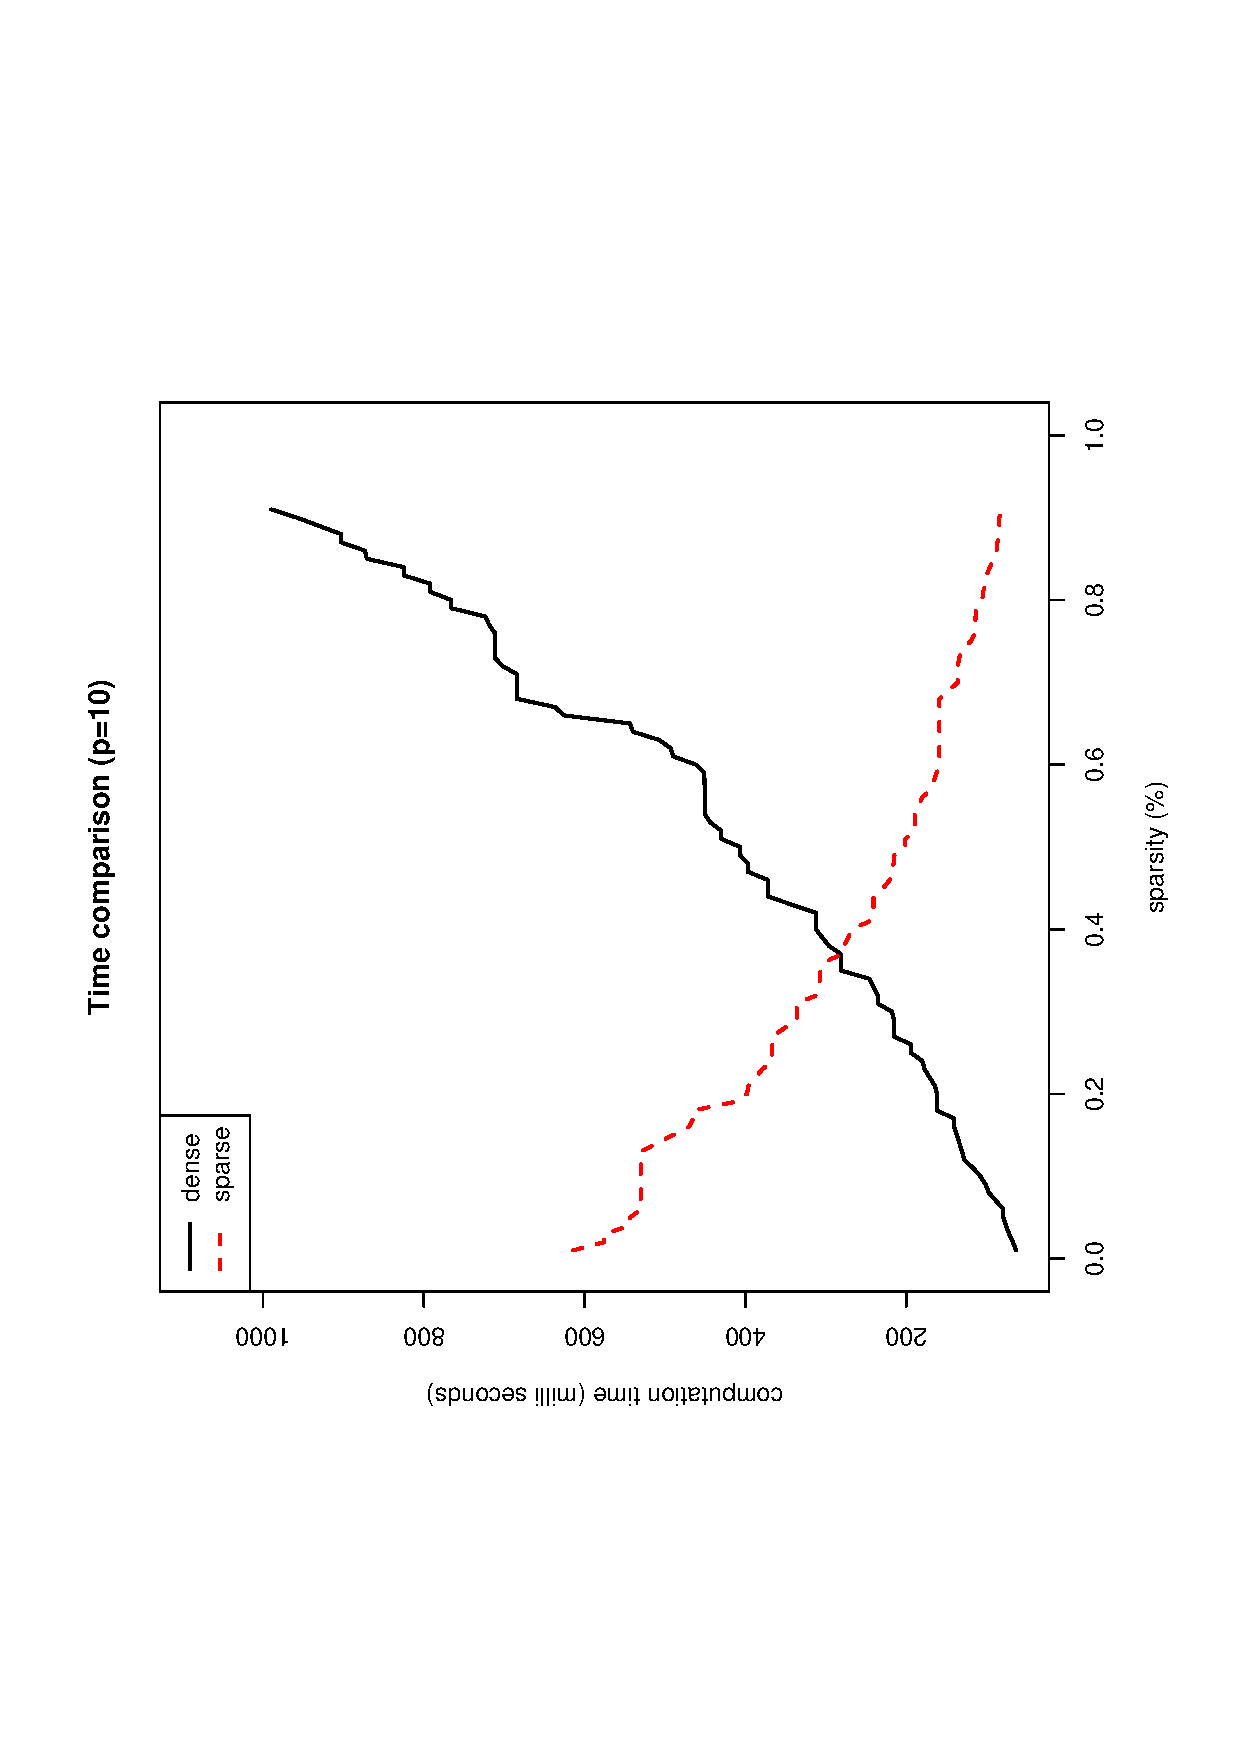
\includegraphics[scale=0.28,angle=270]{timeComparison_p10.pdf}
\\
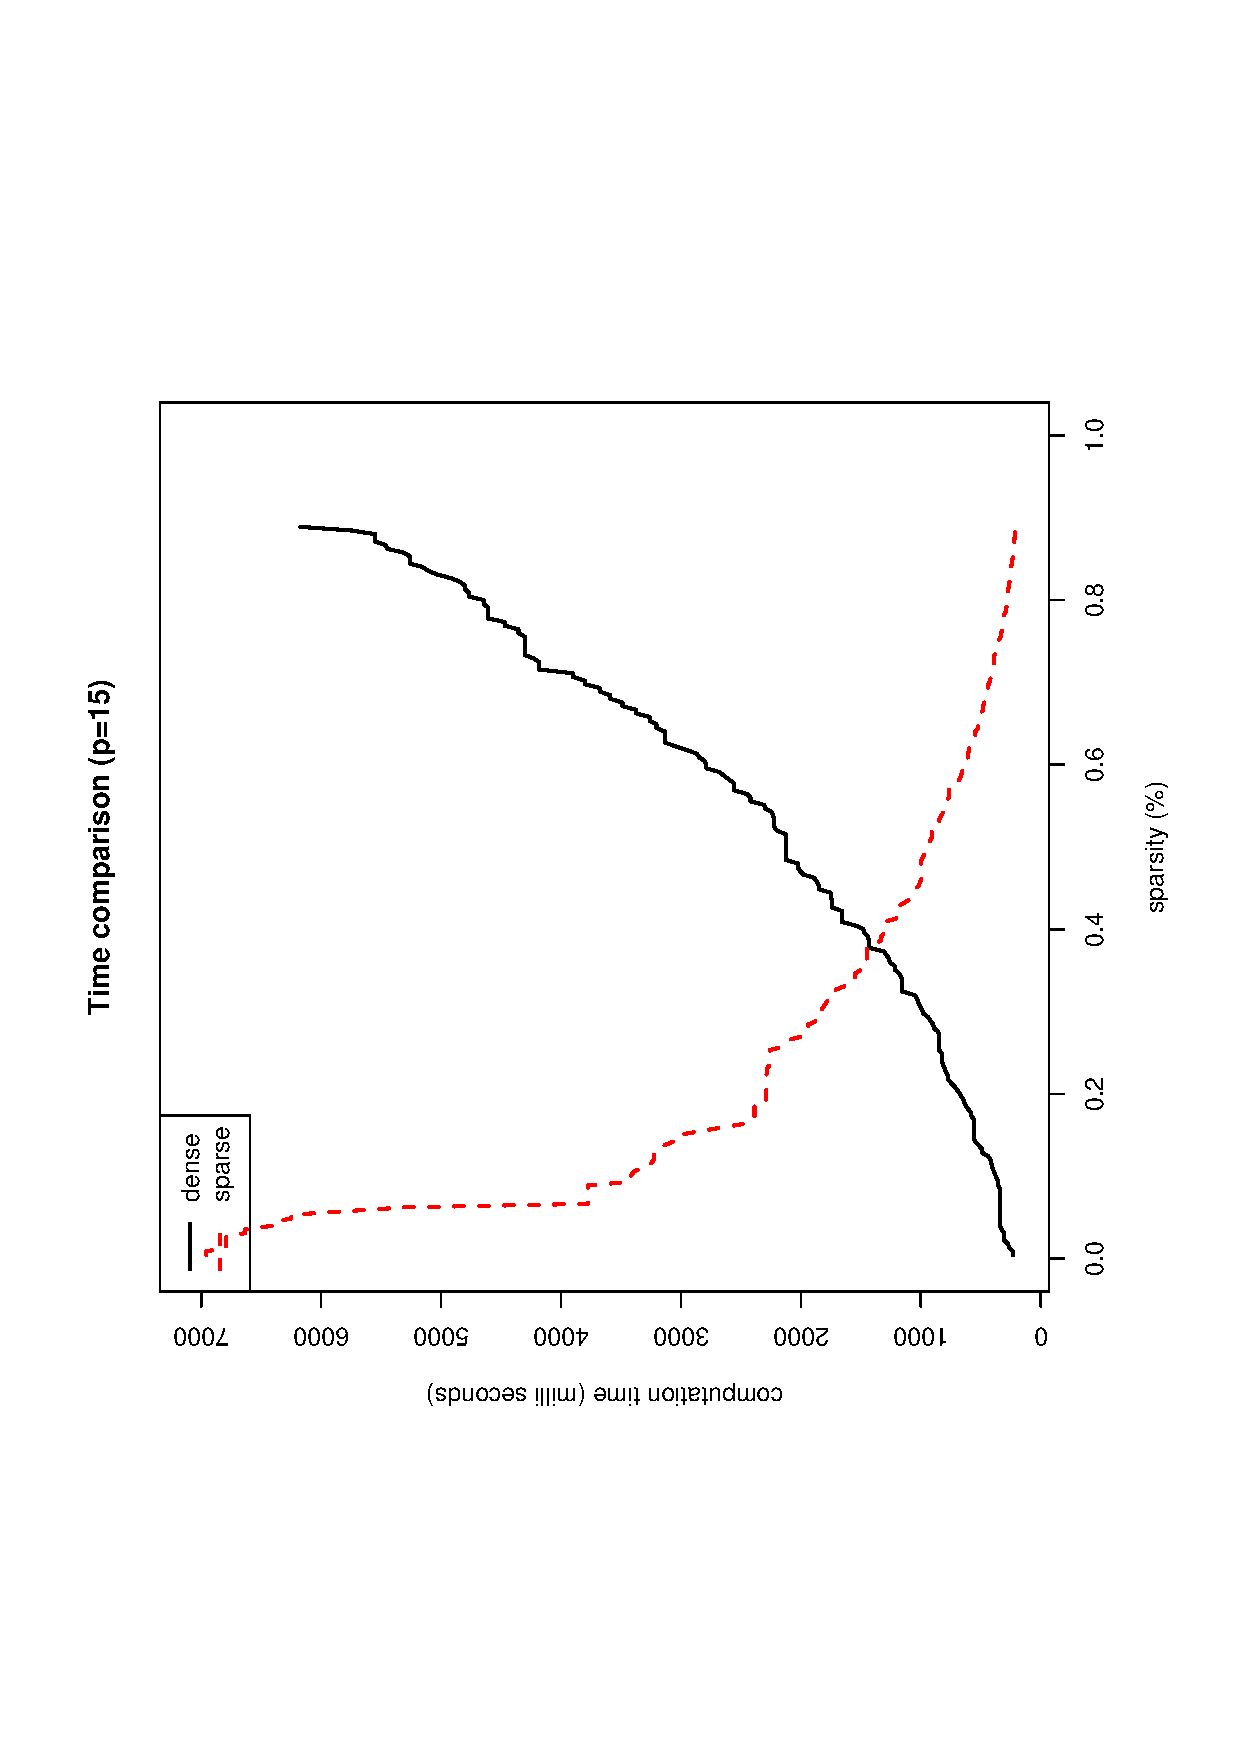
\includegraphics[scale=0.28,angle=270]{timeComparison_p15.pdf} &
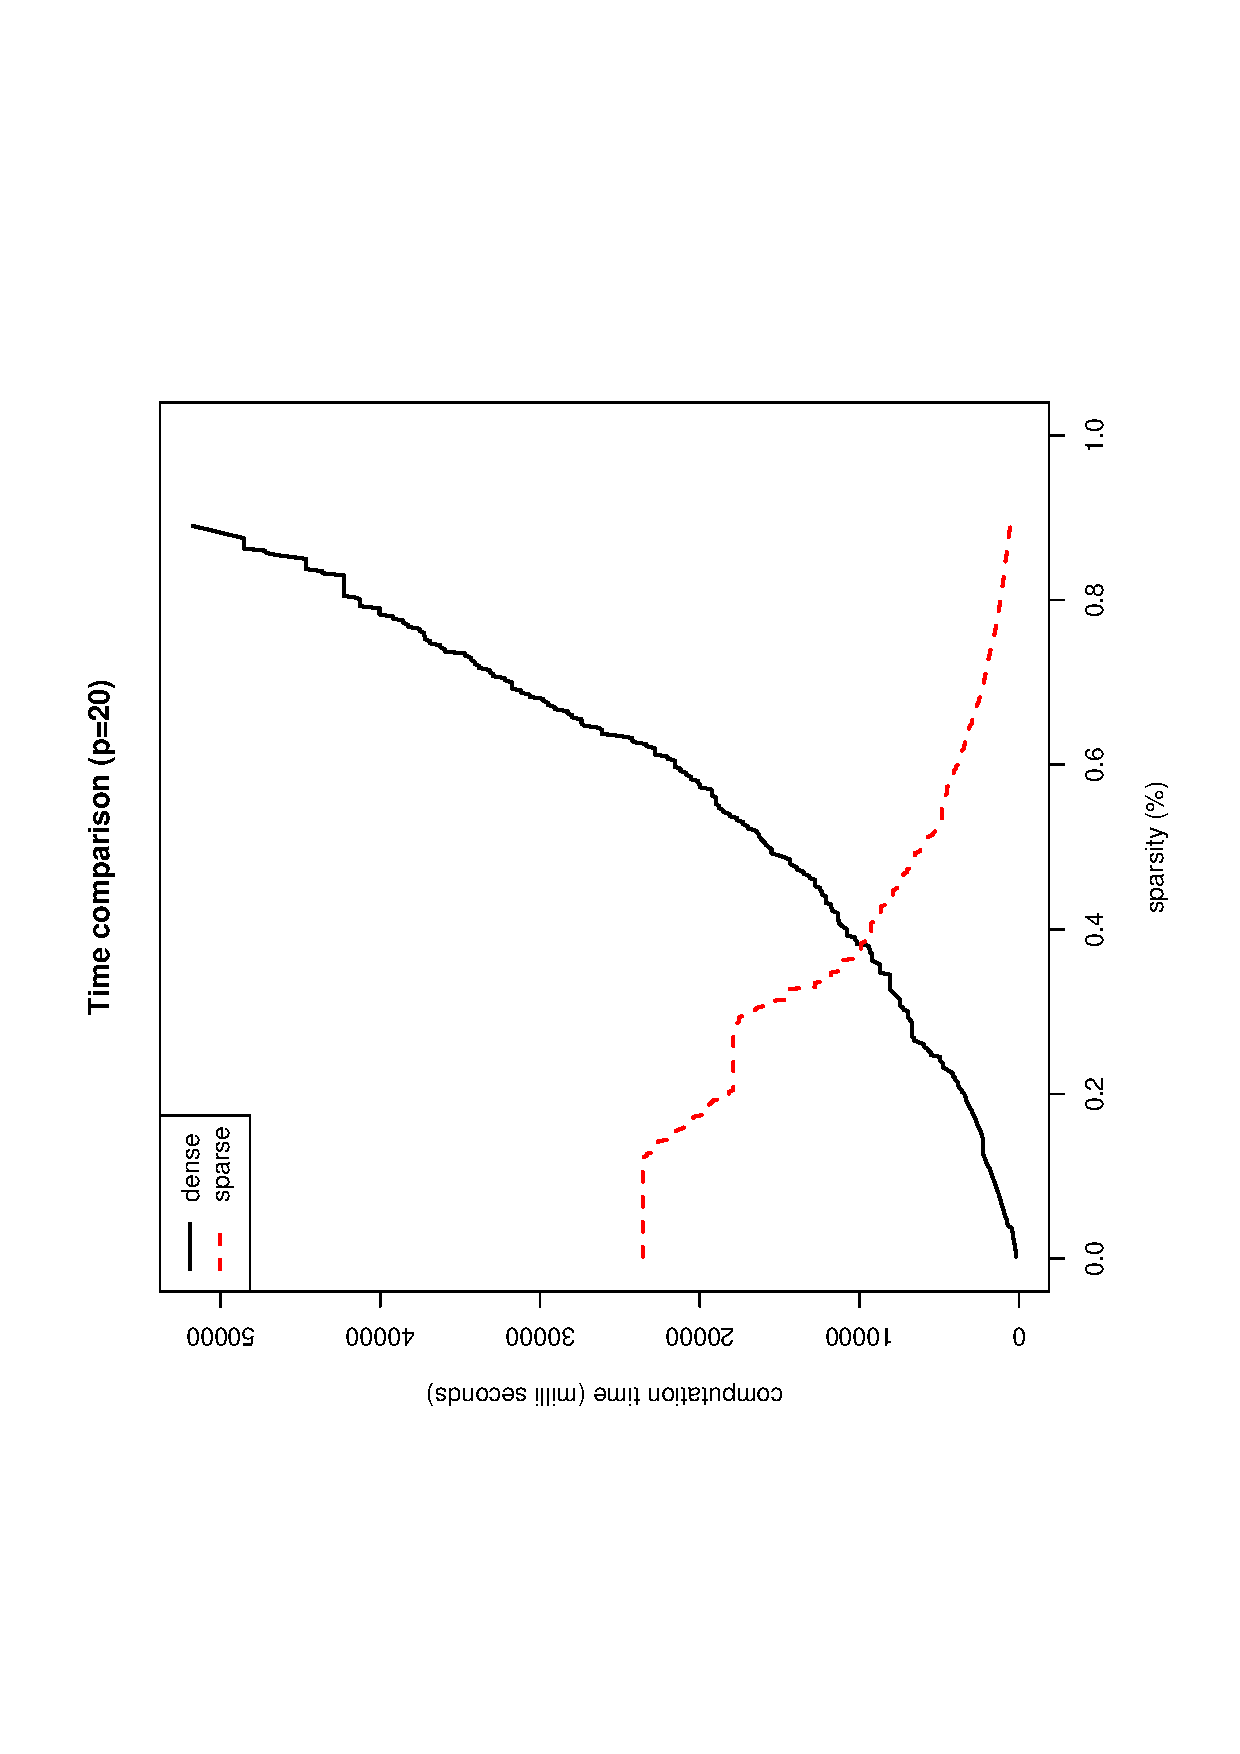
\includegraphics[scale=0.28,angle=270]{timeComparison_p20.pdf}
\\
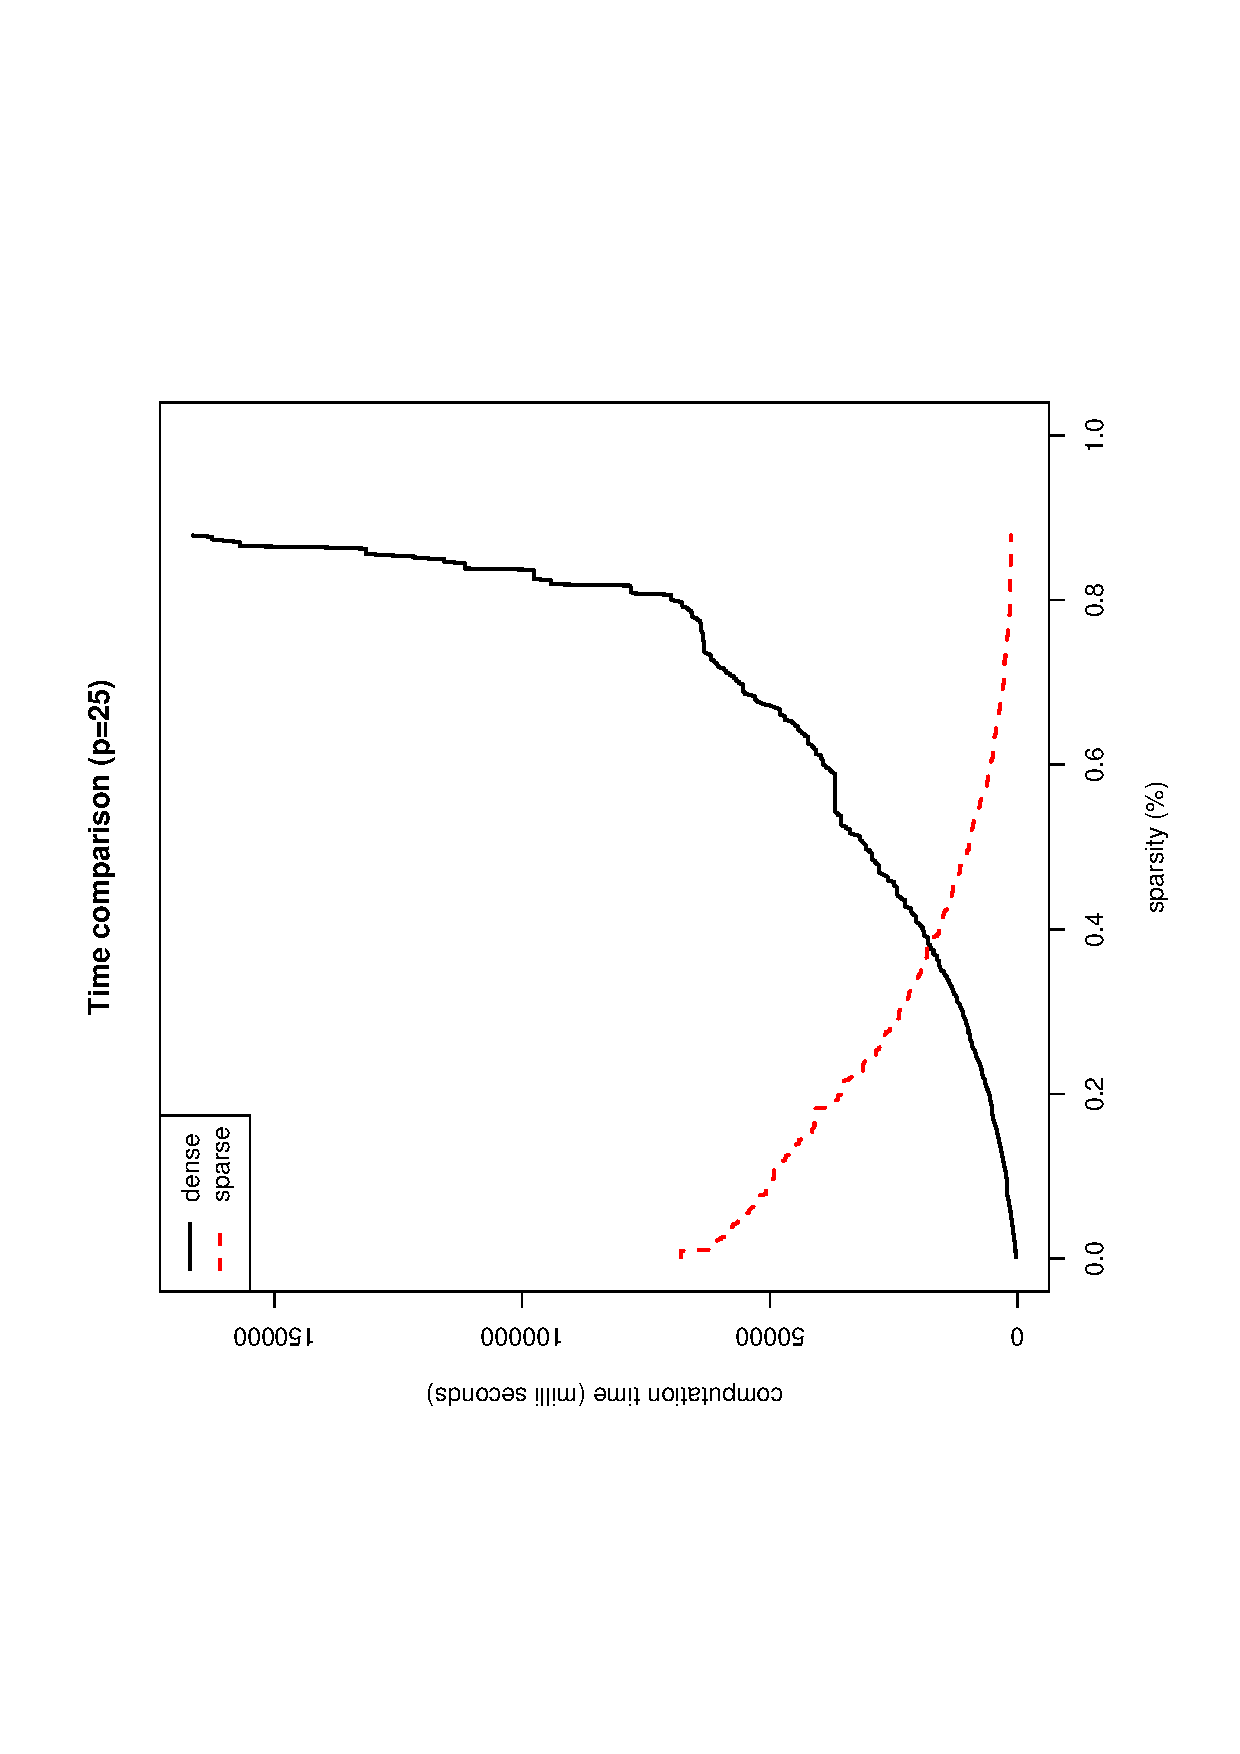
\includegraphics[scale=0.28,angle=270]{timeComparison_p25.pdf} &
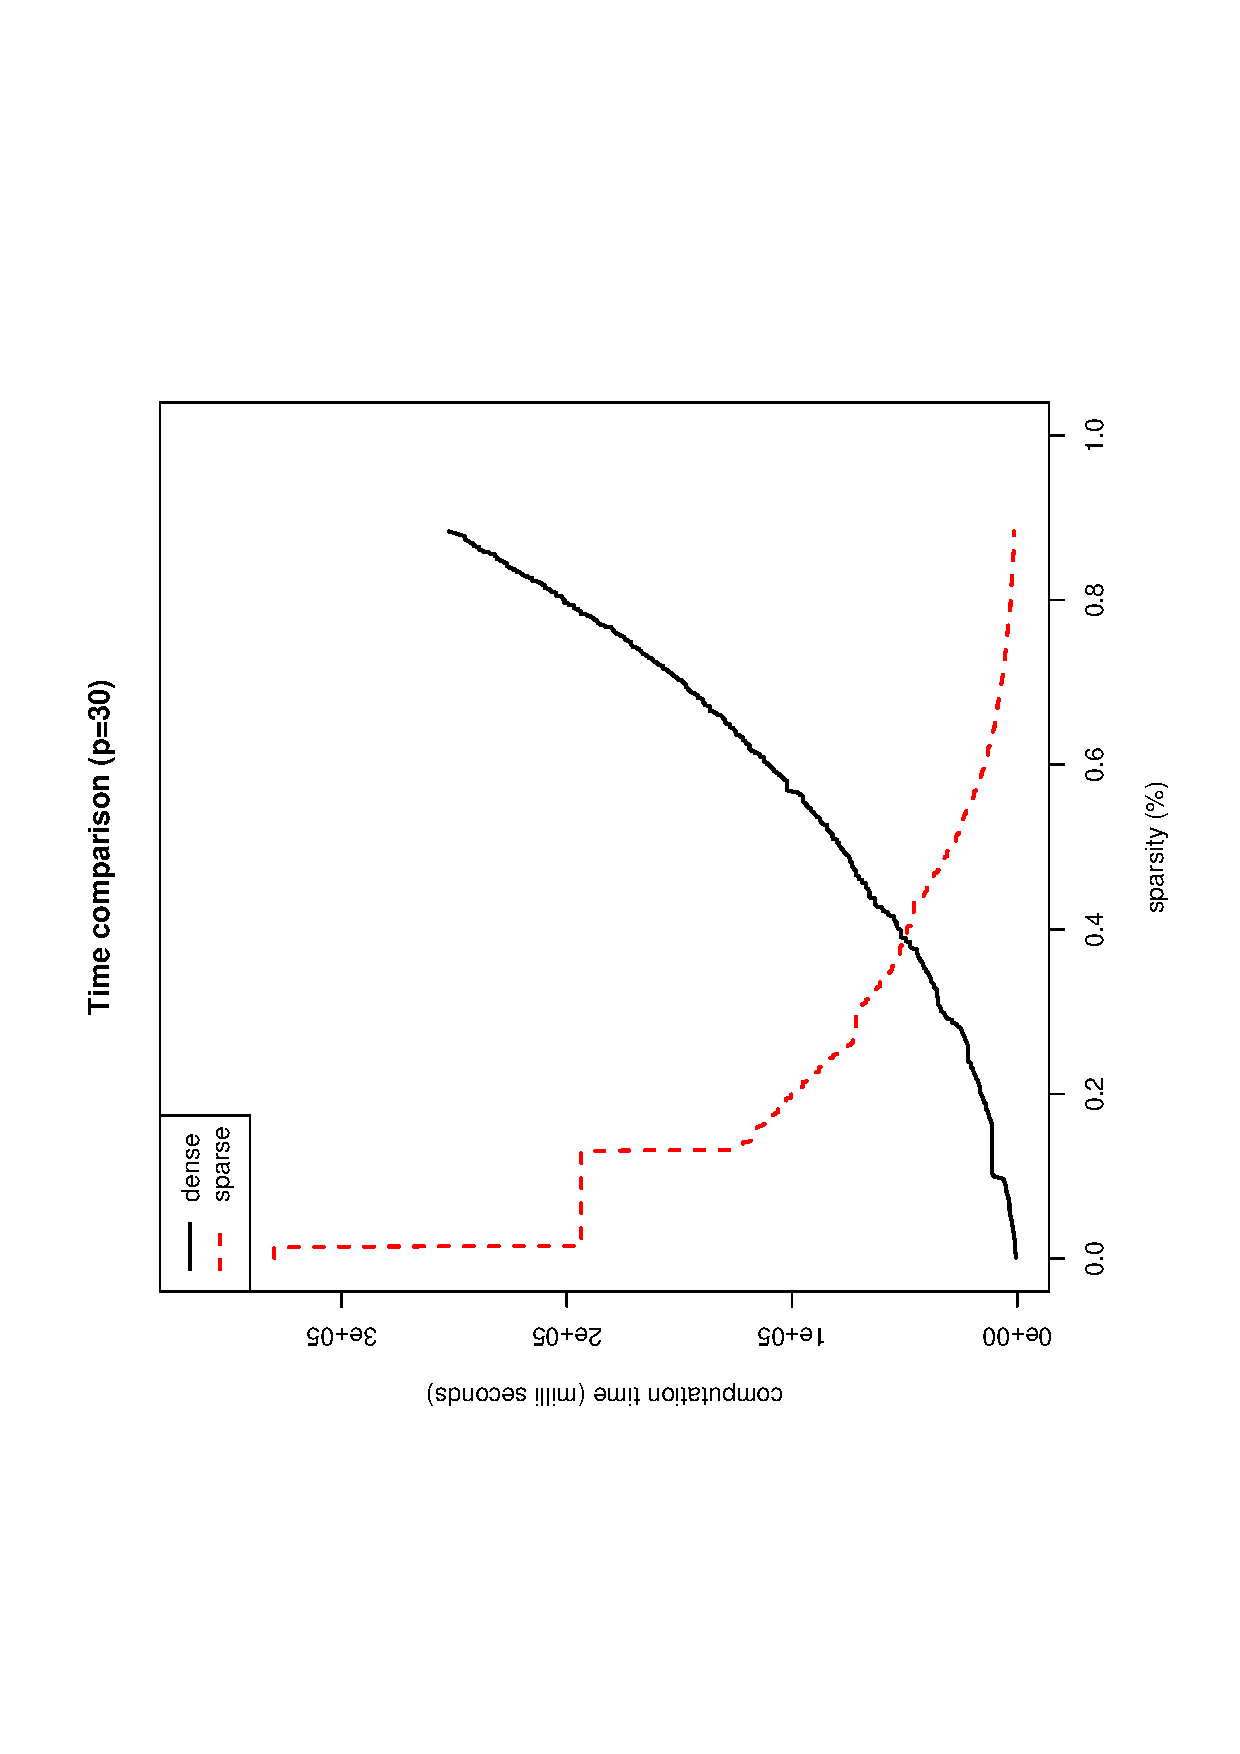
\includegraphics[scale=0.28,angle=270]{timeComparison_p30.pdf}
\end{tabular}
\caption{The computational costs of evaluating the estimator of $\mathbf{A}$ with known support for two plotted against the sparsity percentage of the support. Two different implementations are evaluated: for a dense (few zeros; black, solid line) and sparse (many zeros; red, dashed line) support. Computation times were evaluated using the {\tt microbenchmark}-package (\cite{Mersmann2014}). }
\label{figSM:timeComparison}
\end{figure}




\newpage
\section{Decomposable graph illustration}
Figure \ref{fig.decomposableGraphIllustration} shows an example of a decomposable graph and its decomposition. Clearly, every path between the two cliques runs via the separator. Furthermore, both cliques and separator are complete subgraphs. Hence, they form a decomposition of the graph. Figure \ref{figSM:examplesOfChordalGraph} containing two additional examples of decomposable graph: the tree and the chain graph.

\begin{figure}[h!]
\begin{center}
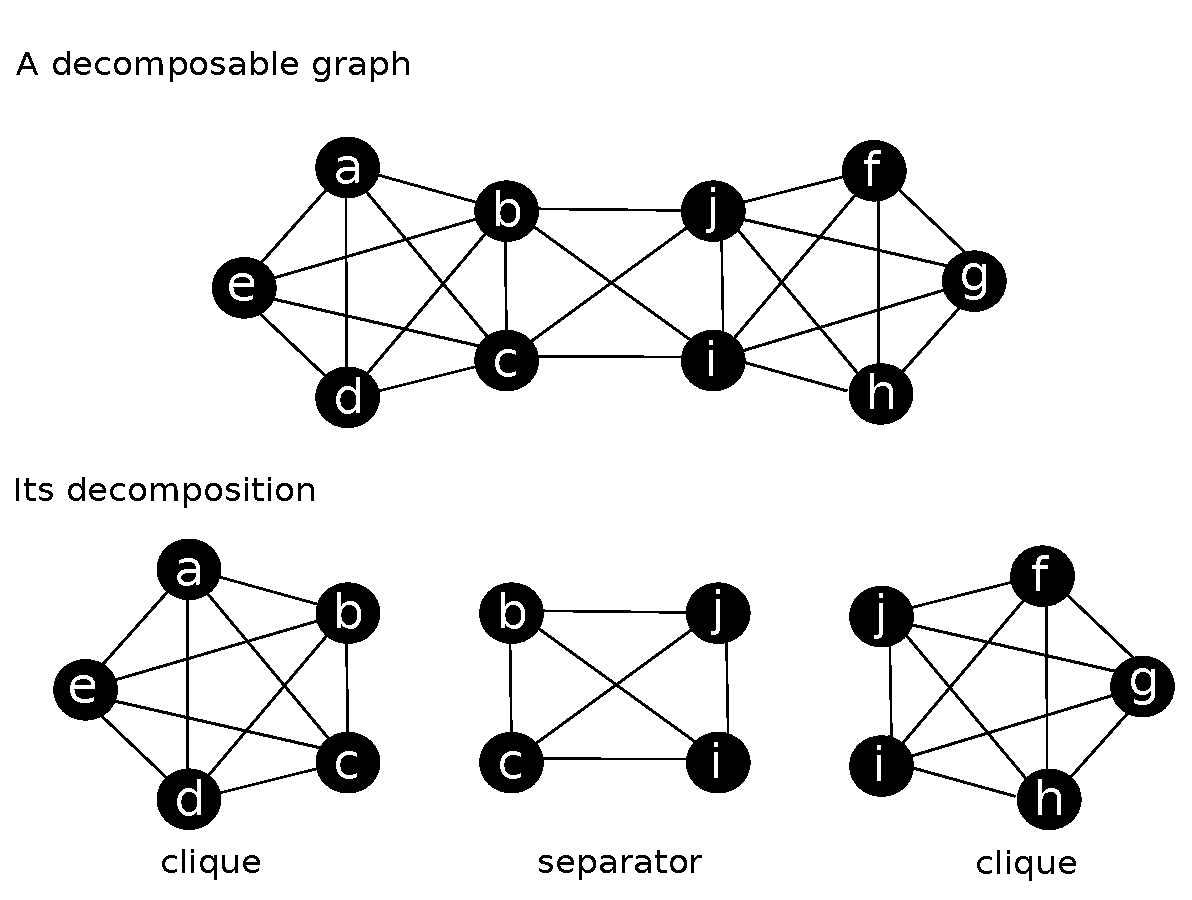
\includegraphics[angle=0, scale=0.45]{DecomposableGraph.eps}
\end{center}
\caption{The top row shows a decomposable graph. The bottom row displays its decomposition in terms of the two cliques, comprising vertices $\{a, b, c, d, e\}$ and $\{f, g, h, i, j\}$ and the edges connecting them, and a separator with vertices $\{b, c, i, j\}$ and the edges connecting them.
\label{fig.decomposableGraphIllustration}}
\end{figure}

\begin{figure}[h!]
\centering
\begin{tabular}{ll}
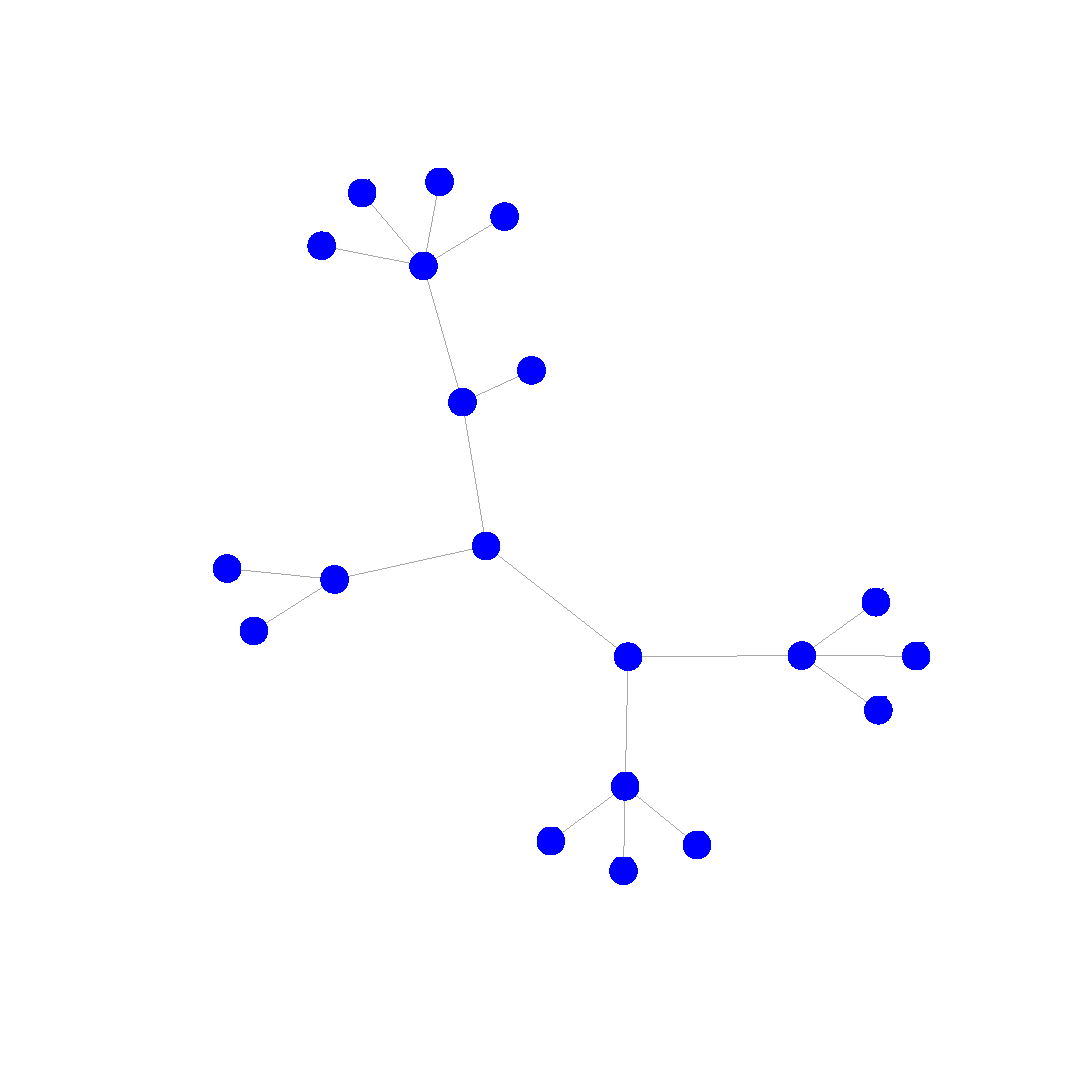
\includegraphics[angle=0, scale=0.4]{chordalGraph_tree_graph.eps} &
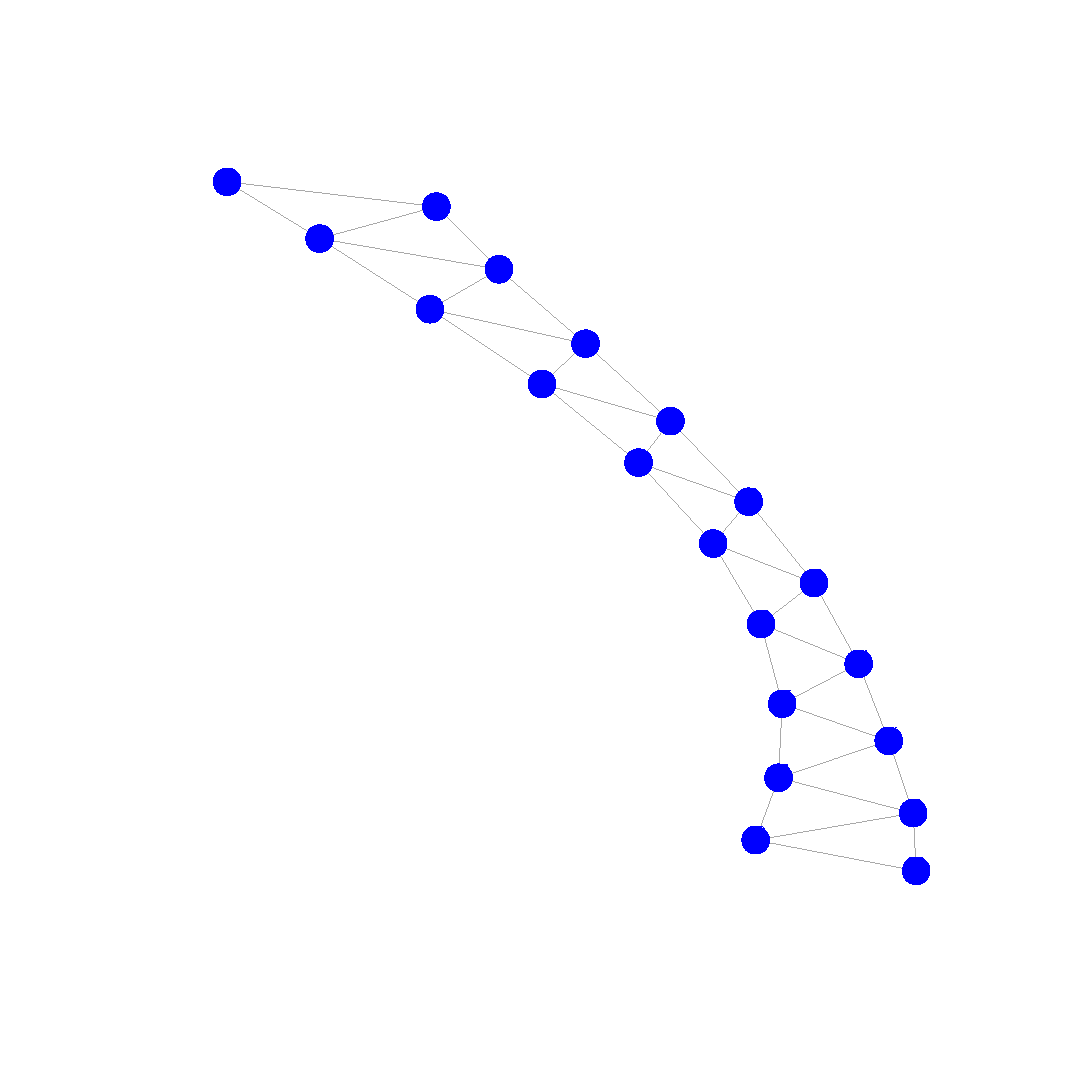
\includegraphics[angle=0, scale=0.4]{chordalGraph_chain_graph.eps}
\end{tabular}
\caption{Two examples of decomposable graphs: the tree and a chain graph. }
\label{figSM:examplesOfChordalGraph}
\end{figure}



\newpage
\section{Initial estimate of $\mathbf{\Omega}$ with chordal support}
Under the assumption of a decomposable conditional independence graph $\mathcal{G}$, the ridge ML estimator of $\mathbf{\Omega}_{\varepsilon}$ can be expressed in limiting cases ($\lambda_{\omega}=0$, $\lambda_{\omega}=\infty$ and $\mathcal{S} = \emptyset$) as a combination of the ridge ML estimators of the cliques and separators that decompose $\mathcal{G}$. Fully analogous to unpenalized case specified by Proposition 5.9 of \cite{Lauritzen1996} but with the unpenalized marginal ML covariance estimates of cliques and separators replaced by their penalized counterparts.

To derive the ridge ML estimator for the aforementioned limiting cases, note by direct observation that the decomposability of the support of $\mathbf{\Omega}_{\varepsilon}$ implies:
\begin{eqnarray}
\nonumber
\mbox{tr}  [ (\mathbf{\Omega}_{\varepsilon} - \mathbf{\Omega}_0)^\top (\mathbf{\Omega}_{\varepsilon} - \mathbf{\Omega}_0)]
& = & \sum_{\mathsfit{C} \in \mathcal{C}} \mbox{tr} \{ [ (\mathbf{\Omega}_{\varepsilon})_{\mathsfit{C},\mathsfit{C}} - (\mathbf{\Omega}_0)_{\mathsfit{C}, \mathsfit{C}} ]^{\top} [(\mathbf{\Omega}_{\varepsilon})_{\mathsfit{C},\mathsfit{C}} - (\mathbf{\Omega}_0)_{\mathsfit{C}, \mathsfit{C}}] \}
\\
\label{form.reformulatedRidgePanelty}
& &  \, - \, \sum_{\mathsfit{S} \in \mathcal{S}} \mbox{tr} \{ [ (\mathbf{\Omega}_{\varepsilon})_{\mathsfit{S},\mathsfit{S}} - (\mathbf{\Omega}_0)_{\mathsfit{S}, \mathsfit{S}} ]^{\top} [(\mathbf{\Omega}_{\varepsilon})_{\mathsfit{S}, \mathsfit{S}} - (\mathbf{\Omega}_0)_{\mathsfit{S}, \mathsfit{S}}] \},
\end{eqnarray}
in which $\mathbf{\Omega}_0$ is assumed to share its support with $\mathbf{\Omega}_{\varepsilon}$. For square, symmetric $\mathbf{S}_{\varepsilon} \succeq$, $\mathbf{\Omega}_{\varepsilon} \succ 0$, and $\mathbf{\Omega}_0 \succ 0$ of arbitrary but equal dimensions define
\begin{eqnarray*}
\mathcal{L}_{\omega}^{\mbox{{\tiny pen}}}(\mathbf{S}_{\varepsilon}, \mathbf{\Omega}_{\varepsilon}, \mathbf{\Omega}_0, \lambda_{\omega}) & = & \frac{1}{2} n (\mathcal{T} - 1) \big\{ \log| \mathbf{\Omega}_{\varepsilon} |   - \mbox{tr}  ( \mathbf{S}  \mathbf{\Omega}_{\varepsilon} ) - \lambda_{\omega} \mbox{tr}  [ (\mathbf{\Omega}_{\varepsilon} -\mathbf{\Omega}_0)^{\top} (\mathbf{\Omega}_{\varepsilon} - \mathbf{\Omega}_0) ] \big\}.
\end{eqnarray*}
Using the reformulated ridge penalty (\ref{form.reformulatedRidgePanelty}) together with iterative application of Lemma 5.5. of \cite{Lauritzen1996}, which decomposes the unpenalized log-likelihood in a linear combination of those of the cliques and separators, the loss function for $\mathbf{\Omega}_{\varepsilon}$ can then be rewritten to:
\begin{eqnarray} 
\nonumber
\sum_{\mathsfit{C} \in \mathcal{C}} \mathcal{L}^{\mbox{{\tiny pen}}}_{\omega}[(\mathbf{S}_{\varepsilon})_{\mathsfit{C},\mathsfit{C}}, (\mathbf{\Omega}_{\varepsilon})_{\mathsfit{C},\mathsfit{C}}, (\mathbf{\Omega}_{0})_{\mathsfit{C},\mathsfit{C}}, \lambda_{\omega}] 
\\
\label{form.decomposedPenLoglik}
& &  \, - \, \sum_{\mathsfit{S} \in \mathcal{S}} \nu(\mathsfit{S}) \mathcal{L}^{\mbox{{\tiny pen}}}_{\omega} [(\mathbf{S}_{\varepsilon})_{\mathsfit{S},\mathsfit{S}}, (\mathbf{\Omega}_{\varepsilon})_{\mathsfit{S},\mathsfit{S}},
(\mathbf{\Omega}_{0})_{\mathsfit{S},\mathsfit{S}}, \lambda_{\omega}],
\end{eqnarray}
where $\nu(\mathsfit{S})$ is the number of times separator $\mathsfit{S}$ forms the intersection of two neighboring cliques.

Recall from the main text that, when $\mathcal{G}$ decomposes into cliques $\mathsfit{C}_1$, $\mathsfit{C}_2$ and $\mathsfit{S}$, the proposed ridge ML estimator is:
\begin{eqnarray*}
\hspace{-1.5cm}\widehat{\mathbf{\Omega}}_{\varepsilon}(\lambda_{\omega}) & = & 
\left(
\begin{array}{lll}
\, [\widehat{\mathbf{\Omega}}_{\varepsilon}^{({\mathsfit{C}_1})}(\lambda_{\omega})]_{\mathsfit{C}_1 \setminus \mathsfit{S}, \mathsfit{C}_1 \setminus \mathsfit{S}} & [\widehat{\mathbf{\Omega}}_{\varepsilon}^{({\mathsfit{C}_1})}(\lambda_{\omega})]_{\mathsfit{C}_1 \setminus \mathsfit{S}, \mathsfit{S}} & \mathbf{0}_{|\mathsfit{C}_1 \setminus \mathsfit{S}| \times |\mathsfit{C}_2 \setminus \mathsfit{S}|}
\\
\, [\widehat{\mathbf{\Omega}}_{\varepsilon}^{(\mathsfit{C}_1)}(\lambda_{\omega})]_{\mathsfit{S}, \mathsfit{C}_1 \setminus \mathsfit{S}} & [\widehat{\mathbf{\Omega}}_{\varepsilon}^{({\mathsfit{C}_1})}(\lambda_{\omega})]_{\mathsfit{S}, \mathsfit{S}} + [\widehat{\mathbf{\Omega}}_{\varepsilon}^{({\mathsfit{C}_2})}(\lambda_{\omega})]_{\mathsfit{S}, \mathsfit{S}} - \widehat{\mathbf{\Omega}}_{\varepsilon}^{(\mathsfit{S})}(\lambda_{\omega}) & [\widehat{\mathbf{\Omega}}_{\varepsilon}^{({\mathsfit{C}_2})}(\lambda_{\omega})]_{\mathsfit{S}, \mathsfit{C}_2 \setminus \mathsfit{S}}
\\
\, \mathbf{0}_{|\mathsfit{C}_2 \setminus \mathsfit{S}| \times |\mathsfit{C}_1 \setminus \mathsfit{S}|} & [\widehat{\mathbf{\Omega}}_{\varepsilon}^{({\mathsfit{C}_2})}(\lambda_{\omega})]_{\mathsfit{C}_2 \setminus \mathsfit{S}, \mathsfit{S}} & [\widehat{\mathbf{\Omega}}_{\varepsilon}^{({\mathsfit{C}_2})}(\lambda_{\omega})]_{\mathsfit{C}_2 \setminus \mathsfit{S}, \mathsfit{C}_2 \setminus \mathsfit{S}}
\end{array}
\right),
\end{eqnarray*}
where $\widehat{\mathbf{\Omega}}_{\varepsilon}^{({\mathsfit{C}_1})}(\lambda_{\omega})$, $\widehat{\mathbf{\Omega}}_{\varepsilon}^{({\mathsfit{C}_1})}(\lambda_{\omega})$ and $\widehat{\mathbf{\Omega}}_{\varepsilon}^{({\mathsfit{S}})}(\lambda_{\omega})$ are the marginal ridge ML covariance estimators for cliques $\mathsfit{C}_1$, $\mathsfit{C}_2$ and separator $\mathsfit{S}$. Note that each of these marginal estimator satisfy the marginal estimating equation, e.g.:
\begin{eqnarray*}
[\widehat{\mathbf{\Omega}}_{\varepsilon}^{({\mathsfit{C}_1})}(\lambda_{\omega})]^{-1} - \lambda_{\omega} \widehat{\mathbf{\Omega}}_{\varepsilon}^{({\mathsfit{C}_1})}(\lambda_{\omega}) & = & (\mathbf{S}_{\varepsilon})_{\mathsfit{C}_1, \mathsfit{C}_1} - \lambda_{\omega} (\mathbf{\Omega}_{0})_{\mathsfit{C}_1, \mathsfit{C}_1},
\end{eqnarray*}
confer \cite{Wieringen2016} for details.


To show that this estimator maximizes (in the three limiting cases) the ridge penalized log-likelihood under the assumption of a decomposable conditional independence graph, we study this penalized log-likelihood in the vicinity of the proposed estimator. Let a $\mathbf{\Delta}$ be a $p \times p$ dimensional matrix and $\gamma$ a constant close to but unequal to zero. Consider a single summand of the penalized log-likelihood (\ref{form.decomposedPenLoglik}), say, that of the first clique. It may then, after noting that $\log(\mathbf{A} + \varepsilon \mathbf{B}) = \log( \mathbf{A}) + \varepsilon \mathbf{A}^{-1} \mathbf{B} + \mathcal{O}(\varepsilon^2)$ and $\log( | \mathbf{A} |)  = \mbox{tr} [ \log(\mathbf{A})]$, be approximated by:
\begin{eqnarray*}
& & \hspace{-1cm} \mathcal{L}^{\mbox{{\tiny pen}}}_{\omega} \big\{ (\mathbf{S}_{\varepsilon})_{\mathsfit{C}_1,\mathsfit{C}_1}, [\widehat{\mathbf{\Omega}}_{\varepsilon}(\lambda_{\omega}) ]_{\mathsfit{C}_1,\mathsfit{C}_1} + \gamma \, (\mathbf{\Delta})_{\mathsfit{C}_1,\mathsfit{C}_1}, (\mathbf{\Omega}_{0})_{\mathsfit{C}_1,\mathsfit{C}_1}, \lambda_{\omega} \big\}
\\
& \approx & \log \big\{ | [\widehat{\mathbf{\Omega}}_{\varepsilon}(\lambda_{\omega}) ]_{\mathsfit{C}_1,\mathsfit{C}_1} | \big\}
 - \, \mbox{tr}  \big\{ (\mathbf{S}_{\varepsilon})_{\mathsfit{C}_1,\mathsfit{C}_1}  [\widehat{\mathbf{\Omega}}_{\varepsilon}(\lambda_{\omega})]_{\mathsfit{C}_1,\mathsfit{C}_1} \big\}
\\
& &
- \frac{1}{2} \lambda_{\omega} \mbox{tr}  \Big(  \big\{ [\widehat{\mathbf{\Omega}}_{\varepsilon}(\lambda_{\omega})]_{\mathsfit{C}_1,\mathsfit{C}_1} - (\mathbf{\Omega}_{0})_{\mathsfit{C}_1,\mathsfit{C}_1} \big\}^{\top} \big\{ [\widehat{\mathbf{\Omega}}_{\varepsilon}(\lambda_{\omega})]_{\mathsfit{C}_1,\mathsfit{C}_1} - (\mathbf{\Omega}_{0})_{\mathsfit{C}_1,\mathsfit{C}_1} \big\} \Big)
\\
& & + \, \gamma \, \mbox{tr} \Big[ \Big(
\big\{ [\widehat{\mathbf{\Omega}}_{\varepsilon}(\lambda_{\omega})]_{\mathsfit{C}_1,\mathsfit{C}_1} \big\}^{-1} -
\big\{ [\widehat{\mathbf{\Omega}}_{\varepsilon}(\lambda_{\omega})]^{-1} \big\}_{\mathsfit{C}_1,\mathsfit{C}_1}
\Big) ( \mathbf{\Delta})_{\mathsfit{C}_1,\mathsfit{C}_1} \Big) \Big]
\\
& & - \frac{1}{2} \gamma^2 \lambda_{\omega} \mbox{tr}  \big\{  [  (\mathbf{\Delta})_{\mathsfit{C}_1,\mathsfit{C}_1} ]^{\top}  ( \mathbf{\Delta})_{\mathsfit{C}_1,\mathsfit{C}_1}  \big\},
\end{eqnarray*}
in which we also used the estimating equation.

Only the latter two summands of this approximation of the penalized log-likelihood of the clique involve $\gamma$. Now consider the three boundary cases separately:
\begin{compactitem}
\item When $\lambda_{\omega} = 0$ the summands in the approximation stemming from the penalty vanish and the claim is warranted by Lemma 5.5 of \cite{Lauritzen1996}.

\item When $\mathcal{S} = \emptyset$, the precision matrix is block diagonal and the blocks can be estimated marginally. This implies $[(\widehat{\mathbf{\Omega}}_{\varepsilon})_{\mathsfit{C}_1,\mathsfit{C}_1} ]^{-1} =
[(\widehat{\mathbf{\Omega}}_{\varepsilon})^{-1}]_{\mathsfit{C}_1,\mathsfit{C}_1}$ and ensures that the first summand involving $\gamma$ vanishes. As the second summand can only contribute negatively to the log-likelihood for any $\gamma \not= 0$, the proposed estimator maximizes the log-likelihood.

\item When $\lambda_{\omega}$ tends to infinity, the second summand involving $\gamma$ dominates the other. For these dominant summands:
\begin{eqnarray*}
\mbox{tr}  ( \mathbf{\Delta}^\top \mathbf{\Delta})
& = & \sum_{\mathsfit{C} \in \mathcal{C}} \mbox{tr} \{ [ (\mathbf{\Delta})_{\mathsfit{C},\mathsfit{C}}]^{\top} (\mathbf{\Delta})_{\mathsfit{C},\mathsfit{C}} \}
\, - \, \sum_{\mathsfit{S} \in \mathcal{S}} \mbox{tr} \{ [ (\mathbf{\Delta})_{\mathsfit{S},\mathsfit{S}}]^{\top} (\mathbf{\Delta})_{\mathsfit{S}, \mathsfit{S}} \}.
\end{eqnarray*}
The total contribution of these terms to the log-likelihood is thus negative for any choice of $\gamma$ other than zero.

\end{compactitem}
Hence, the proposed estimator indeed maximizes the penalized log-likelihood in the three limiting cases.

\newpage
\section{Path analysis illustration}
The path analysis of autocovariance is illustrated by means of a toy example. Consider a VAR(1) model parametrized by:
\begin{eqnarray*}
\mathbf{\nu} \, \, \, = \, \, \,
\left(
\begin{array}{rrr}
0
\\
0
\\
0
\end{array}
\right),
\quad \mathbf{A} \, \, \, = \, \, \,
\left(
\begin{array}{rrr}
\rfrac{1}{2} & \rfrac{1}{2} & \rfrac{1}{2}
\\
0 & 0 & 0
\\
0 & 0 & 0
\end{array}
\right)
\quad \mbox{ and } \quad
\mathbf{\Sigma}_{\varepsilon} & = &
\left(
\begin{array}{rrr}
1 & \rfrac{1}{5} & \rfrac{1}{5}
\\
\rfrac{1}{5} & 1 & 0
\\
\rfrac{1}{5} & 0 & 1
\end{array}
\right)^{-1}.
\end{eqnarray*}
The top row of Figure \ref{fig.TSCGpathAnalysis} displays the corresponding time series chain graph.

The autocovariance between $Y_{1,t}$ and $Y_{1,t+1}$ (dropping the sample index for notational clarity) is: $\mbox{Cov}(Y_{1,t}, Y_{1,t+1}) = (\mathbf{\Sigma}_{\varepsilon} \mathbf{A}^{\top})_{1,1} = 0.326087$. From the time series chain graph it is immediate that $Y_{1,t}$ and $Y_{1,t+1}$  are connected by three paths (visualized by the bottom row of Figure \ref{fig.TSCGpathAnalysis}): \textit{i)} $Y_{1,t} \rightarrow Y_{1,t+1}$, \textit{ii)} $Y_{1,t} \rightarrow Y_{2,t} \rightarrow Y_{1,t+1}$, and \textit{iii)} $Y_{1,t} \rightarrow Y_{3,t} \rightarrow Y_{1,t+1}$. The	 covariance between $Y_{1,t}$ and $Y_{1,t+1}$ can now be decomposed into the contributions of each of these paths. Using the decomposition of the autocovariance in terms of the paths' contributions from the main text one obtains: $0.5434783$ (for $Y_{1,t} \rightarrow Y_{1,t+1}$), $-0.1086957$ (for $Y_{1,t} \rightarrow Y_{2,t} \rightarrow Y_{1,t+1}$) and $-0.1086957$ (for $Y_{1,t} \rightarrow Y_{3,t} \rightarrow Y_{1,t+1}$). These contributions indeed sum to $0.326087$, which equals $\mbox{Cov}(Y_{1,t}, Y_{1,t+1})$.

\begin{figure}[b!]
\begin{center}
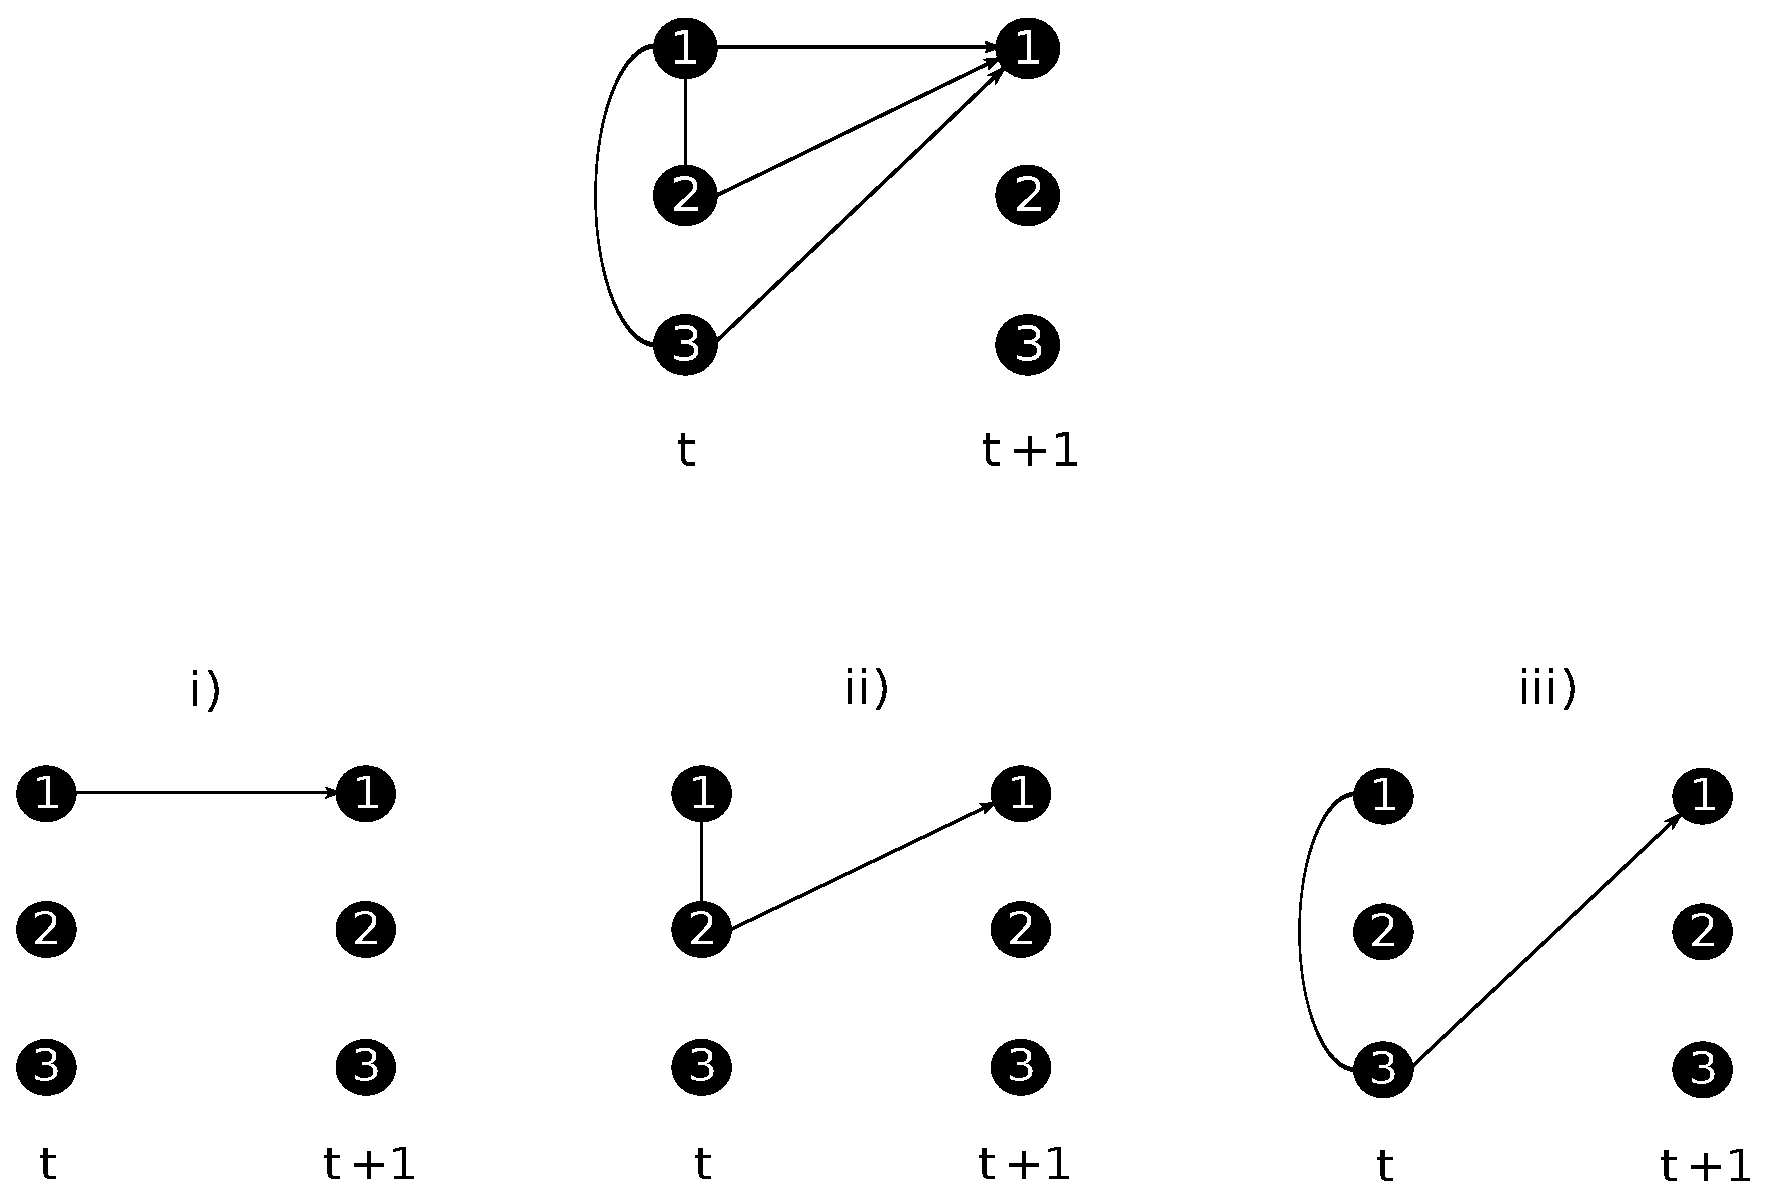
\includegraphics[angle=0, scale=0.5]{TSCG_pathExample2.eps}
\end{center}
\caption{The top row shows the time series chain graph of the toy model. The bottom row displays the three paths in the time series chain graph connecting the first variate between to consecutive time points.
\label{fig.TSCGpathAnalysis}}
\end{figure}



\newpage
\section{Design of time-course studies in GEO}
\cite{Ernst2005} observed that more than $80\%$ of time-course gene expression microarray data sets have 8 or fewer number of time points. This reference being somewhat out of date, we conducted our own survey using the GEO data base. Using the search terms ``time course'', ``cancer'', ``human'',  ``cell line'', ``gene expression'', ``microarray'', 85 studies where selected (at June 23, 2015). From the resulting list we excluded studies involving hematological tumors and data set GSE762 with a rather intricate experimental design (among other a time component). Finally, 63 studies satisfy these criteria, involving cell lines of various cancer types (breast, colon, prostate, ovarian, kidney and lung) and were mainly conducted using Affymetrix gene expression arrays (confer Table 3.1 Figure \ref{figSM:GEOhist} shows histograms of the number of time-points $\mathcal{T}$ and individuals $n$ (left panels) and the scatterplot of these study characteristics. From the provided table and histograms we conclude that a reasonable optimistic and simultaneously empirically maximum number of time-points and individuals are 10 and 5, respectively.
\\
\mbox{ }
\\
\mbox{ }
\\
\mbox{ }

\begin{figure}[h!]
\centering
\begin{tabular}{ccc}
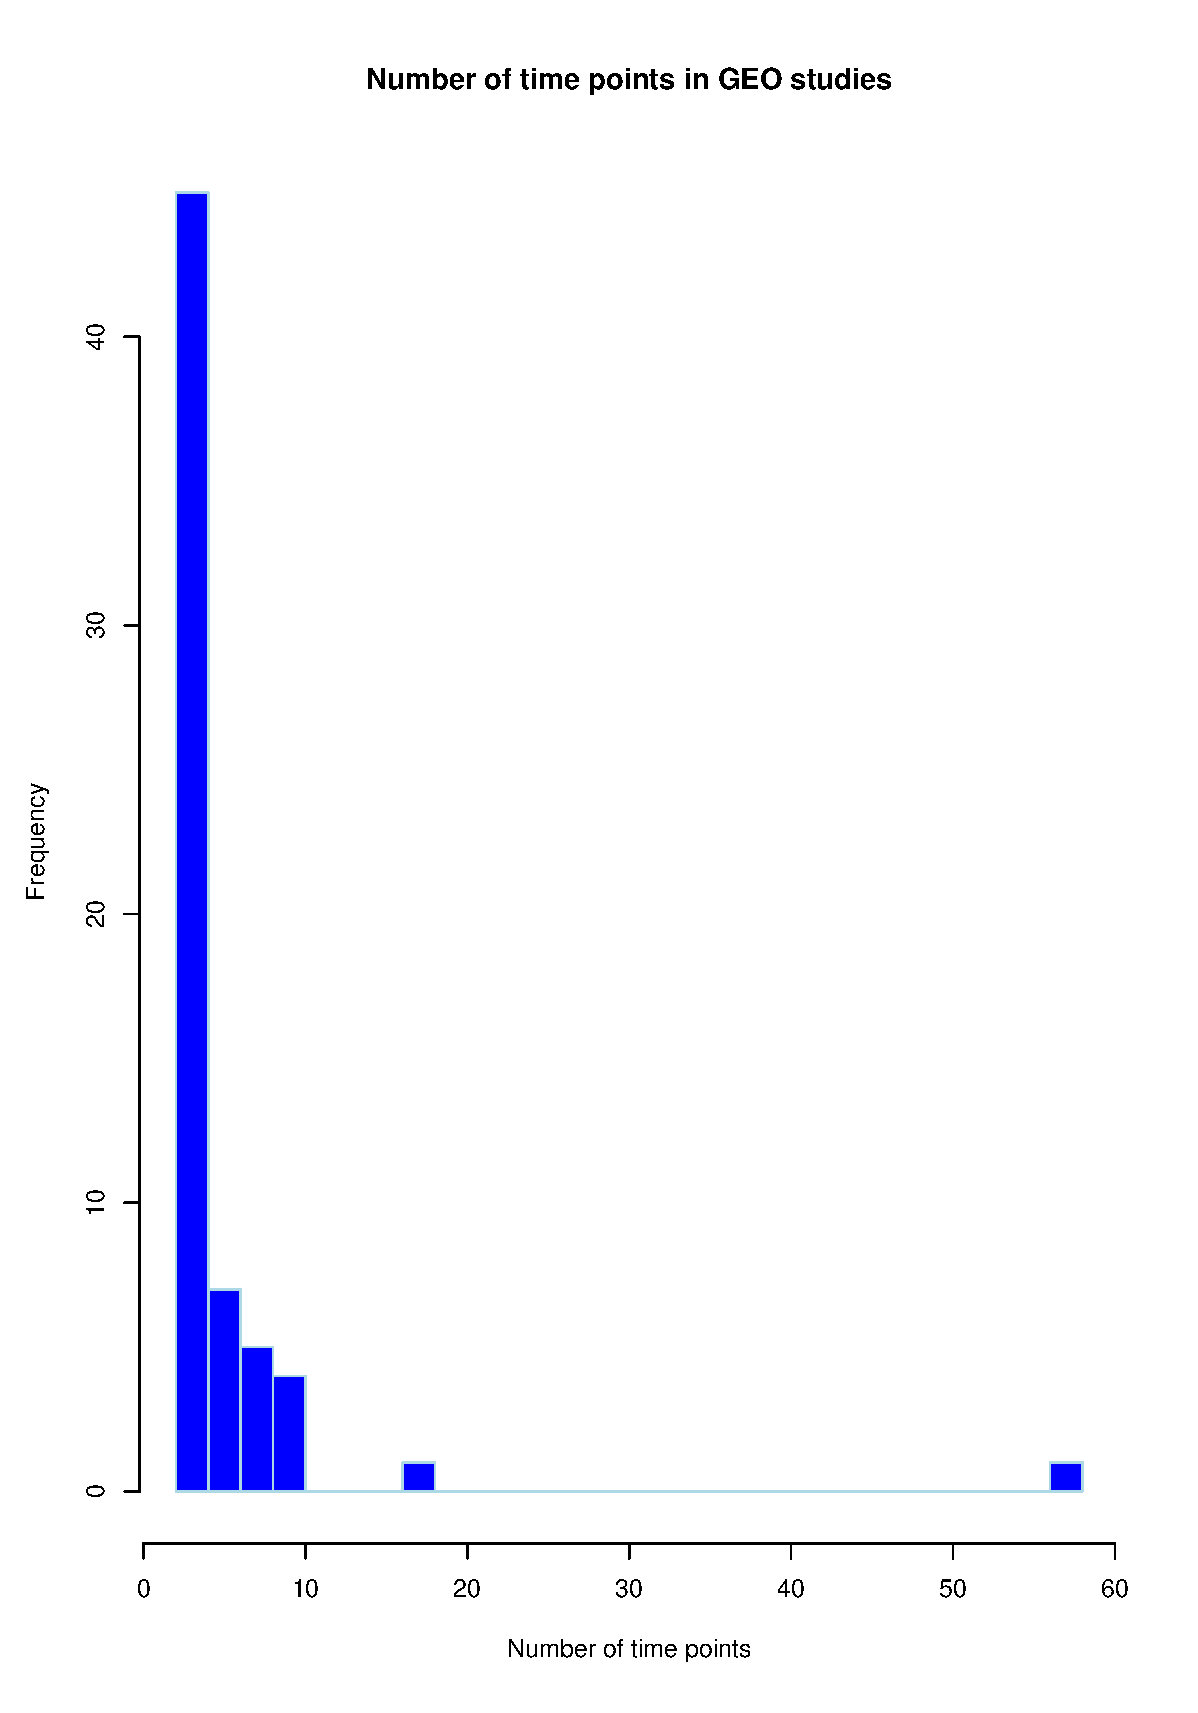
\includegraphics[scale=0.24]{GEOtime.eps} &
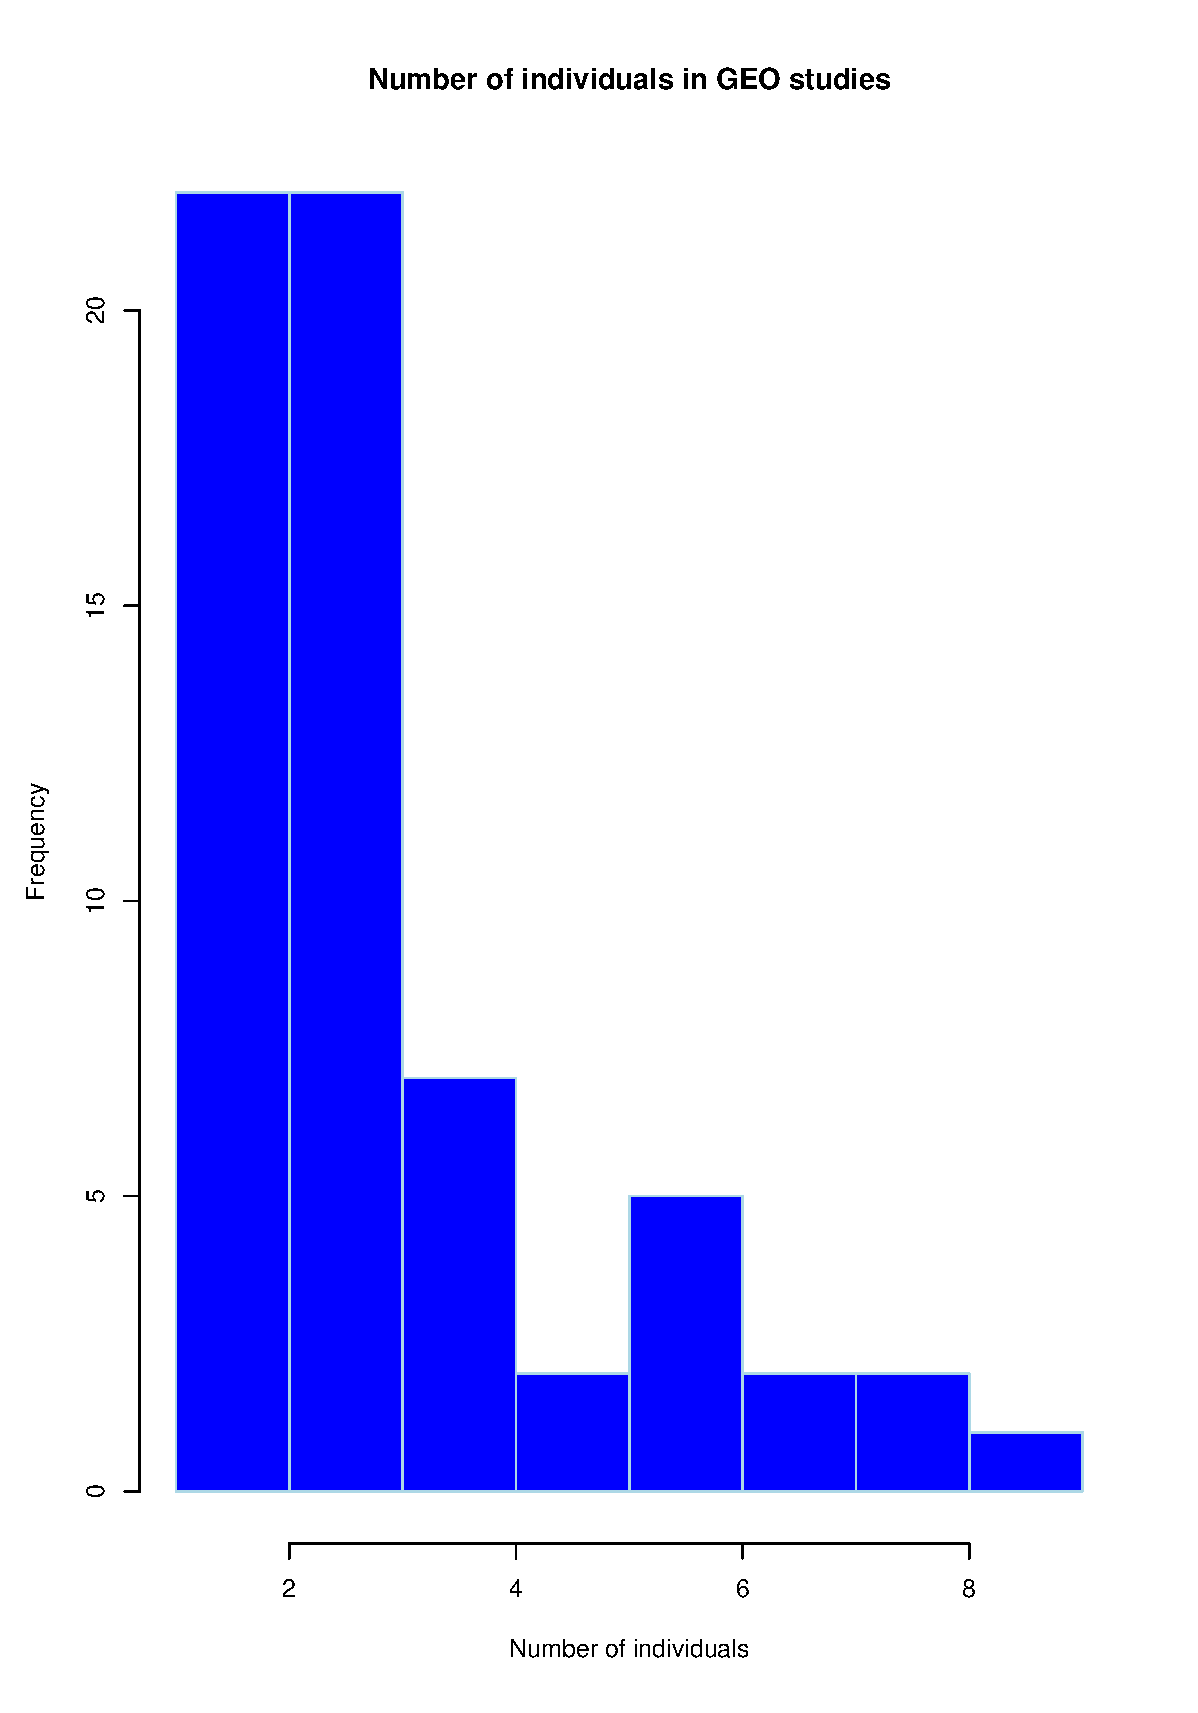
\includegraphics[scale=0.24]{GEOind.eps} &
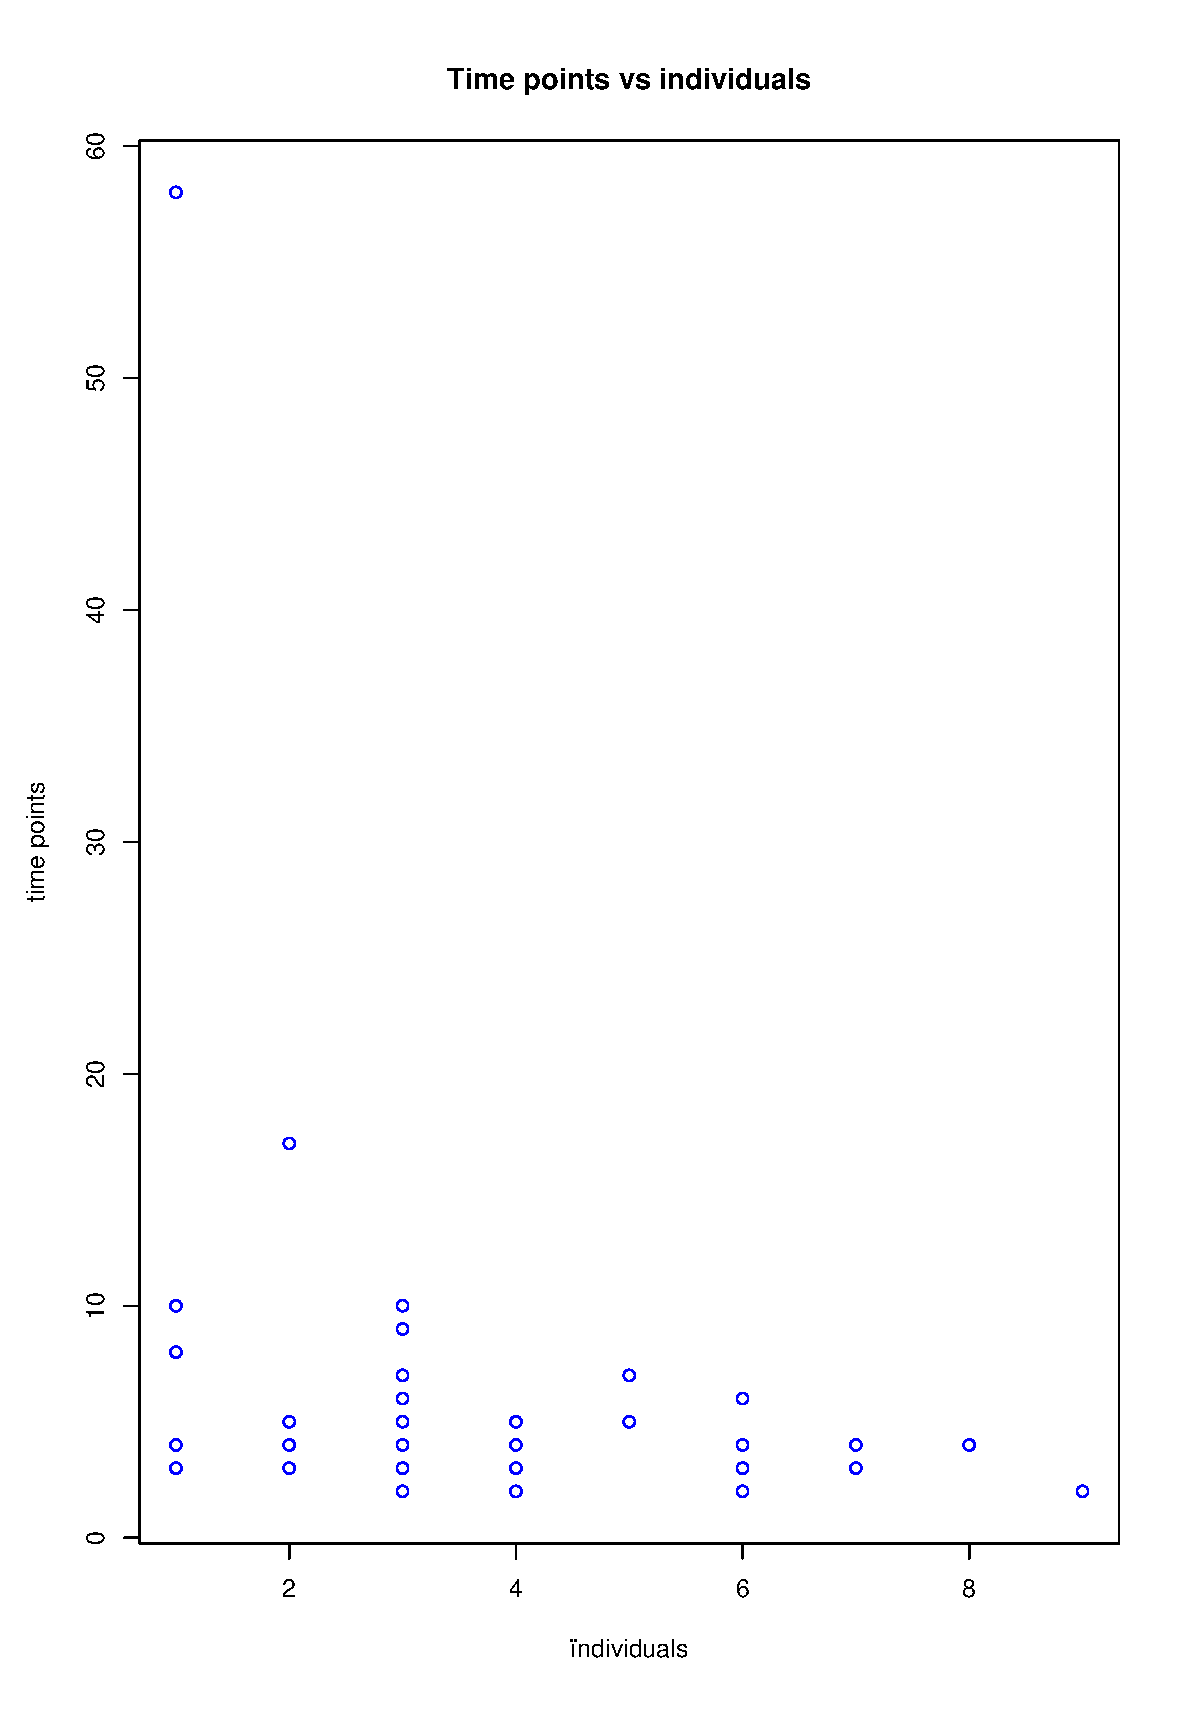
\includegraphics[scale=0.24]{GEOscat.eps}\\
\end{tabular}
\caption{Number of time-points and observations in microarray time-course gene expression studies from GEO database. Left panel presents the histogram of number of time-points, while the middle panel shows the histogram of the number of observations (cell lines) in GEO studies. The right panel plots the number of time points against the number of individuals.}
\label{figSM:GEOhist}
\end{figure}



% Histograms of the number of time-points (left panel) and observations (right panel) of GEO  gene expression microarray studies with a time-course set-up.




\begin{table}
{\scriptsize
\begin{tabular}{lrrrlll}
\hline
& & & & & & \\
\textbf{data}	&	\textbf{\# time}	&	\textbf{\# individuals}	&	\textbf{\# treatments}	&	\textbf{cancer}	&	\textbf{organism}	&	\textbf{platform}	\\
\textbf{set ID}	&	\textbf{points}	&		&	&	\textbf{type}	&		& \\
& & & & & &
\\
\hline
& & & & & &
\\
GSE7868	&	3	&	3	&	1	&	prostate	&	human	&	Affymetrix	\\
GDS2626	&	4	&	7	&	2	&	breast	&	human	&	Affymetrix	\\
GSE29917	&	7	&	5	&	3	&	breast	&	human	&	Agilent	\\
GSE13009	&	17	&	2	&	2	&	breast	&	human	&	Affymetrix	\\
GDS4367	&	5	&	3	&	1	&	colon	&	mouse	&	Affymetrix	\\
GDS4121	&	3	&	1	&	1	&	prostate	&	human 	&	Affymetrix	\\
GDS4110	&	9	&	3	&	1	&	prostate	&	human	&	Affymetrix	\\
GDS4063	&	2	&	9	&	3	&	breast	&	human	&	Affymetrix	\\
GDS4052	&	2	&	6	&	3	&	breast	&	human	&	Affymetrix	\\
GDS3910	&	3	&	2	&	3	&	breast	&	human	&	Affymetrix	\\
GDS3887	&	4	&	4	&	2	&	bladder	&	mouse	&	Affymetrix	\\
GDS3872	&	3	&	3	&	2	&	ovarian	&	human	&	Affymetrix	\\
GDS3761	&	3	&	4	&	2	&	prostate	&	human	&	Affymetrix	\\
GDS3710	&	9	&	3	&	1	&	epithelial	&	human	&	Affymetrix	\\
GDS3517	&	4	&	3	&	4	&	melanoma	&	human	&	Affymetrix	\\
GDS3484	&	2	&	3	&	2	&	breast	&	human	&	Affymetrix	\\
GDS3792	&	3	&	2	&	2	&	ovarian	&	human	&	Affymetrix	\\
GDS3358	&	5	&	2	&	2	&	prostate	&	human	&	Affymetrix	\\
GDS3319	&	3	&	1	&	3	&	thyroid	&	human	&	Affymetrix	\\
GDS3285	&	4	&	3	&	1	&	breast	&	human 	&	Affymetrix	\\
GDS3283	&	2	&	6	&	2	&	breast	&	human	&	Affymetrix	\\
GDS3116	&	58	&	1	&	2	&	breast	&	human	&	Affymetrix	\\
GDS3111	&	3	&	3	&	2	&	prostate	&	human	&	Affymetrix	\\
GDS2975	&	4	&	2	&	1	&	ovarian	&	human	&	Affymetrix	\\
GDS2810	&	3	&	2	&	2	&	breast	&	human	&	Affymetrix	\\
GDS2604	&	6	&	6	&		&	lung	&	human 	&	Affymetrix	\\
GDS2323	&	3	&	3	&	1	&	breast	&	human 	&	Affymetrix	\\
GDS2097	&	4	&	1	&	2	&	breast	&	human 	&	Affymetrix	\\
GDS2096	&	4	&	1	&	2	&	breast	&	human 	&	Affymetrix	\\
GDS1942	&	8	&	1	&	2	&	colon	&	human	&	Affymetrix	\\
GDS1736	&	2	&	4	&	2	&	prostate	&	human	&	Affymetrix	\\
GDS1627	&	3	&	2	&		&	breast	&	human	&	oligo	\\
GDS848	&	3	&	7	&	3	&	breast	&	human	&	oligo	\\
GDS725	&	10	&	1	&	1	&	prostate	&	human	&	Affymetrix	\\
GDS719	&	4	&	2	&	3	&	prostate	&	human	&	Affymetrix	\\
GDS528	&	3	&	3	&	1	&	colon	&	human	&	Affymetrix	\\
GSE41828	&	5	&	5	&	2	&	prostate	&	human	&	Affymetrix	\\
GSE41680	&	4	&	1	&	2	&	melanoma	&	human	&	Affymetrix	\\
GSE31128	&	4	&	3	&	4	&	breast	&	human 	&	Illumina	\\
GSE28305	&	4	&	2	&	1	&	breast	&	human	&	Affymetrix	\\
GDS4853	&	4	&	3	&	2	&	stomach	&	human	&	Affymetrix	\\
GSE26834	&	2	&	3	&	6	&	breast	&	human	&	Affymetrix	\\
GSE23616	&	3	&	3	&	2	&	ovarian	&	human	&	Affymetrix	\\
GSE20361	&	8	&	1	&	1	&	breast	&	human	&	Affymetrix	\\
GSE23845	&	4	&	4	&	1	&	bladder	&	human	&	Affymetrix	\\
GSE15947	&	3	&	4	&	3	&	prostate	&	human	&	Affymetrix	\\
GSE18494	&	4	&	3	&	3	&	breast	&	human	&	Affymetrix	\\
GSE17708	&	10	&	3	&	2	&	lung	&	human	&	Affymetrix	\\
GSE11428	&	3	&	3	&	6	&	prostate	&	human	&	Affymetrix	\\
GSE16424	&	4	&	6	&	2	&	ovarian	&	human	&	Affymetrix	\\
GSE13525	&	3	&	4	&	2	&	ovarian	&	human	&	Affymetrix	\\
GSE13059	&	4	&	8	&	1	&	colon	&	human	&	Affymetrix	\\
GSE8772	&	3	&	2	&	1	&	melanoma	&	human	&	Affymetrix	\\
GSE8702	&	7	&	3	&	1	&	prostate	&	human	&	Affymetrix	\\
GSE9936	&	2	&	3	&	16	&	breast	&	human	&	Affymetrix	\\
GSE9826	&	6	&	3	&	3	&	ovarian	&	human	&	Affymetrix	\\
GSE8057	&	5	&	4	&	8	&	ovarian	&	human	&	Affymetrix	\\
GSE6013	&	5	&	2	&	3	&	lung	&	human 	&	Affymetrix	\\
GSE6930	&	3	&	6	&	4	&	ewing sarcoma	&	human	&	Affymetrix	\\
GSE6653	&	4	&	2	&	1	&	ovarian	&	human	&	Affymetrix	\\
GSE5345	&	7	&	3	&	2	&	prostate	&	human	&	IQUSP	\\
GDS2034	&	4	&	2	&	1	&	ovarian 	&	human	&	Affymetrix	\\
GSE4917	&	4	&	8	&	3	&	breast	&	human 	&	Affymetrix	\\
& & & & & &
\\
\hline & & & & & & \\
\end{tabular}
}
\label{tableSM:GEOdatasets}
\caption{GEO data sets with a time-course design.}
\end{table}




\newpage
\section{Comparison by simulation}
The proposed ridge estimator is compared by means of simulation to (as far as we are aware) the only other method that estimates the VAR(1) model and its associated time series chain graph from high-dimensional data: SparseTSCGM proposed by \cite{Abegaz2013}. SparseTSCGM too estimates parameters of the VAR(1) model in penalized fashion, but employs the smoothly clipped absolute deviation (SCAD, \cite{Fan2001}) penalty on the autoregressive coefficient matrix $\mathbf{A}$ and precision matrix $\mathbf{\Omega}_{\varepsilon}$. As the estimation methods estimate the same VAR(1) model and only differ in the employed penalties, they can readily compared in terms of loss of the estimates and selection of the edges of the time series chain graph.

The ridge and `SCAD' estimators of the VAR(1) model are compared under various choices of the model parameters $\mathbf{A}$ and $\mathbf{\Omega}_{\varepsilon}$, while the number of variates $p$, time points $\mathcal{T}$ and the number of samples $n$ are varied in accordance with a factorial design. We first describe the levels of the factors of the factorial design. The number of variates equals either $p=25$ or $p=50$\footnote{Initially, we also included $p=100$, but the estimation with the SCAD procedure fails to converge for $n=5$ and $T=10$, as is often the case for $p=100$ with larger $n$ and $\mathcal{T}$.}, representing the size of non-trivial but well-defined pathways. Simultaneously, we set $n \in \{5, 15\}$ and $\mathcal{T} \in \{10, 20\}$. We stress that the particular case of $(n=5, \mathcal{T}=10)$ is the most challenging but also most relevant as its design is closest to that which is most prevalent in practice. \cite{Ernst2005} observed that more than $80\%$ of time-course gene expression microarray data sets have 8 or fewer number of time points. This is confirmed by a more recent survey of our own (confer SM III).

We now outline parameter choices of the various VAR(1) models employed in the simulation. Autoregression matrices $\mathbf{A}$ with a hub, cluster, random (each with two sparsity levels: approximately $5\%$ and $25\%$ nonzero elements), and full network structure choices are used. These matrices $\mathbf{A}$ are used in combination with a banded and full precision matrix $\mathbf{\Omega}_{\varepsilon}$ and two data-driven variants. We first detail the various choices of $\mathbf{\Omega}_{\varepsilon}$:
\begin{compactitem}
\item Full $\mathbf{\Omega}_{\varepsilon}$: In the precision matrix $\mathbf{\Omega}_{\varepsilon}$ existing contemporaneous conditional independencies is represented with $\rho=0.5$.

\item Banded $\mathbf{\Omega}_{\varepsilon}$: A banded precision matrix is generated with $(\mathbf{\Omega}_{\varepsilon})_{j_1, j_2} = \rho^{|j_1-j_2|}$ with $\rho=0.5$ for $|j_1-j_2|<3$ and $(\mathbf{\Omega}_{\varepsilon})_{j_1, j_2} = 0$ otherwise.

\item Full but data-driven $\mathbf{\Omega}_{\varepsilon}$: The precision matrix is obtained from a VAR(1) model fitted to data from a time-course gene experiment experiment. The data of the application detailed in the main document are used. The data are limited to genes mapping to the p53 signaling pathway as defined by KEGG. The VAR(1) model is fitted to these pathway data by means of the proposed ridge estimation procedure using penalty parameter values $\lambda_a=0.3, \lambda_{\omega}=0.1$. The thus estimated $\boldsymbol{\Omega}_{\varepsilon}$ is used in the simulation. For the various choice of $p$, the first $p$ genes from the pathway are used in the comparison.
\end{compactitem}

\noindent
For the regression coefficient matrix $\mathbf{A}$ the following variants are employed:
\begin{compactitem}
\item Hub $\mathbf{A}$: All elements of $\mathbf{A}$ are set to zero, except for $(\mathbf{A})_{j_1, j_2}=0.3$ for $j_1=\{d,2d,3d,...\}$ with $j_1>j_2$ and $d=10$ and $d=2$ for the less sparse case). Hence, only a few variates affect (in varying degree) the temporal variation of the others.

\item Cluster $\mathbf{A}$: Eight (most sparse)  or two (less sparse) equally-sized lower-triangular blocks filled with the value 0.3 are aligned along the diagonal. The remaining elements of $\mathbf{A}$ are zero.

\item Random $\mathbf{A}$: A random network is generated, selecting $10\%$  or $50\%$ of the total possible edges, after which the lower triangle is retains, i.e. setting $(\mathbf{A})_{j_1, j_2}=0$ if $j_1<j_2$. Elements of $\mathbf{A}$ are set equal to $0.3$ if the corresponding element in the adjacency matrix of the random network is nonzero.

\item Full data-driven $\mathbf{A}$: The same data set as for the generation of the data-driven $\mathbf{\Omega}_{\varepsilon}$ is used to estimate $\mathbf{A}$. Using these data $\mathbf{A}$ is estimated by the ridge procedure with penalty parameters $\lambda_a=0.3$ and $\lambda_{\omega}=0.1$. The resulting $\mathbf{A}$ is used in the simulation.

\item Sparse data-driven $\mathbf{A}$ is obtained by sparsifying (as outlined in Section 4.1 of the main text) the full data-driven $\mathbf{A}$.
\end{compactitem}
Note that the majority of choices for $\mathbf{A}$ and $\mathbf{\Omega}_{\varepsilon}$ is sparse. This in principle favors the `SCAD' estimation procedure SparseTSCGM.

For (combination of) these choices for the regression parameter matrix $\mathbf{A}$ and precision matrix $\mathbf{\Omega}_{\varepsilon}$, data are simulated in accordance with the VAR(1) model. Data for the first time point $t=1$ are drawn from $\mathcal{N}(\mathbf{0}_{p \times 1}, \mathbf{\Omega}_{\varepsilon}^{-1})$ and for the following time points $t=2,...,T$ data are sampled from $\mathcal{N}(\mathbf{A}\mathbf{Y}_{*,i,t-1},\mathbf{\Sigma}_{\varepsilon})$. In total for each employed combination of the model parameters and design parameters $p$, $n$, $\mathcal{T}$, fifty time series data sets are generated.

For each simulated data set, the VAR(1) model is fitted using both the proposed ridge procedure and the `SCAD'-based method SparseTSCGM. The parameters estimates obtained from both methods are chosen in an identical fashion: using maximization of the leave K-fold-out cross-validated log-likelihood. Instead of removing a single element from the set of design points (as discussed in Section 3.4 of the main document), an individual (cell line) with all its time points is removed at each fold. This is due to the fact that the SparseTSCGM cannot deal with an unbalanced design. Formally, from the set of design points $\mathcal{D} = \{ (t,i): t=1, \ldots, \mathcal{T}, i=1, \ldots, n \}$ we remove a single sample $\mathcal{D}=\{(i): i = 1, \ldots, n\}$ at the time. Resulting parameter estimates of $\mathbf{A}$ and $\boldsymbol{\Omega}_{\varepsilon}$ obtained by SparseTSCGM are sparse, whereas their ridge counterparts are not. This is irrelevant for the loss comparison (for which both a sparse and full matrix can be used). Only comparing the methods with respect to the ability to reconstruct the time series chain graph, the ridge estimates undergo post-estimation sparsification (discussed below).

The ridge and SCAD estimators of $\mathbf{\hat{A}}(\lambda_a)$ and $\widehat{\mathbf{\Omega}}_{\varepsilon}(\lambda_a, \lambda_{\omega})$ are evaluated in terms of their Frobenius loss and their ability to select edges of time series chain graph. The Frobenius loss for (e.g.) a precision  matrix estimate is:
\begin{eqnarray*}
\big\| \widehat{\mathbf{\Omega}}_{\varepsilon}(\lambda_a, \lambda_{\omega}) - \mathbf{\Omega}_{\varepsilon} \big\|_F^2  & = & \sum_{j_1, j_2} \Big\{ \big[ \widehat{\mathbf{\Omega}}_{\varepsilon}(\lambda_a, \lambda_{\omega}) ]_{j_1, j_2} - \big( \mathbf{\Omega}_{\varepsilon}
 )_{j_1, j_2} \Big\}^2.
\end{eqnarray*}
The Frobenius loss for the estimate of $\mathbf{A}$ is defined similarly.


% This sparsification proceeds by retaining in the ridge ML estimate of $\mathbf{A}$ an equal number of edges as produced by the SCAD method. The largest (in an absolute sense) edges are chosen. This sparsification ensures the comparability of the selection of both methods (which is obscured by the use of the empirical Bayes procedure described in the main documents due to differing number of selected edges).

The edge selection ability of the ridge and SCAD estimation methods are compared by means of sensitivity and specificity. When the ridge estimation is augmented with the post-estimation empirical Bayes procedure, the two methods may yield differing number of edges. This may hamper the comparison of their sensitivity and specificity. To facilitate a better comparison, also adhering to the \textit{ceteris paribus} principle, of the two methods in this respect, a simple but different post-estimation edge selection procedure is applied to the ridge estimate. It comprises of selecting the same number of edges as the SCAD method, thus favouring the latter. Having fixed the number of to-be-selected edges, they are selected on the basis of the (absolute) size of the statistic derived from the elements of $\mathbf{A}$ (as pointed out in Section 4.1 the main document) and (standardized) $\widehat{\mathbf{\Omega}}_{\varepsilon}(\lambda_a, \lambda_{\omega})$. This thus means that in each data set for the number of edges selected by the SCAD estimator, we select the same number of largest elements of from the estimate of $\mathbf{A}$.

We first discuss the Frobenius loss comparison. Figures \ref{figSM:Loss25T10N5_5} and \ref{figSM:Loss25T10N5_25} show the Frobenius loss (as boxplots) of the ridge and SCAD estimates of $\mathbf{A}$ (upper panel) with roughly $5\%$ and $25\%$ nonzero elements, respectively, and $\mathbf{\Omega}_{\varepsilon}$ (lower panel) from fifty data sets generated with $p=25$, $T=10$, $n=5$ (the most relevant case empirically), and the various combinations of $\mathbf{A}$ and $\mathbf{\Omega}_{\varepsilon}$. The panels of Figures \ref{figSM:Loss25T10N5_5}  and \ref{figSM:Loss25T10N5_25} reveal that the Frobenius loss of the SCAD estimates of both  $\mathbf{\hat{A}}(\lambda_a)$ and  $\mathbf{\hat{\Omega}_{\varepsilon}}(\lambda_{\omega})$ exceeds that of its ridge counterpart. This observation is consistent over the data sets generated from different choices of the regression coefficient (with all levels of sparsity) and precision matrices. This is confirmed when the VAR(1) model is increased to include $p=50$ variates. The difference in Frobenius loss between the ridge and SCAD estimators grows substantially in favour of the former (confer Figures \ref{figSM:Loss50T10N5_5} and \ref{figSM:Loss50T10N5_25}). When the number of time points $\mathcal{T}$ is increased, the ridge procedure outperforms its SCAD counterpart (as can be witnessed from Figures \ref{figSM:Loss25T20N5_5} and \ref{figSM:Loss25T20N5_25} and Figures \ref{figSM:Loss50T20N5_5} and \ref{figSM:Loss50T20N5_25} representing the `$T=20$, $n=5$'-case with $p=25$ and $p=50$, respectively. 

Increasing the number of samples to the practically non-observed (confer \ref{tableSM:GEOdatasets}) $n=15$ benefits the SCAD estimator in the cases with $p=25$ and the both sparse choices of $\mathbf{A}$ (confer Figures \ref{figSM:Loss25T10N15_5}, \ref{figSM:Loss25T10N15_25}, \ref{figSM:Loss25T20N15_5}, and \ref{figSM:Loss25T20N15_25}). When the number of variates increases to $p=50$ the SCAD still outperforms the ridge estimator in for sparsest $\mathbf{A}$ (Figure \ref{figSM:Loss50T20N15_5}) but roles are reversed when $\mathbf{A}$ contains roughly 25\% nonzero elements (Figure \ref{figSM:Loss25T20N15_25}).

In the latter the superior Frobenius loss of the SCAD estimator is consequence of the sparse $\mathbf{\hat{A}}(\lambda_a)$ and $\boldsymbol{\hat{\Omega}_{\varepsilon}}(\lambda_{\omega})$ which favours the SCAD estimator due to the sparsity of the estimates. This is verified by comparing the ridge and SCAD estimates separately for zero and non-zero elements of $\mathbf{A}$ (not shown). The SCAD estimator performs better for the zero elements, while the ridge estimator outperforms on non-zero elements of $\mathbf{A}$. Only for the hub network does the SCAD estimator generally outperforms the ridge estimator.

We now turn to the sensitivity and specificity of the ridge procedure and that of the SCAD procedure (Figures 
\ref{figSM:RocP25T10N5_5}, \ref{figSM:RocP50T10N5_5},
\ref{figSM:RocP25T20N15_5}, \ref{figSM:RocP50T20N15_5},
\ref{figSM:RocP25T10N5_25}, \ref{figSM:RocP50T10N5_25},
\ref{figSM:RocP25T20N15_25}, and \ref{figSM:RocP50T20N15_25}). Recall, to make the sensitivity and specificity more comparable, the ridge procedure selects (from the largest elements elements of its estimate of $\mathbf{A}$) the same number of edges as found by the SCAD method, thus possibly favouring the latter. In the general picture that then emerges the methods are on a par. For the lower sample sized (and thereby more prevalent) settings a difference is virtually absent. More discriminative power is present when $n=15$ and $mathcal{T}$, but even then no clear winner appear (although then the hub case appears to favour the SCAD method).


%%%%%%%%%%%%%%%%%%%%%%%%%%%%%%%%%%%%%%%%%%%%%%%%%%%%%%%%%%

\begin{figure}[h!]
\centering
\begin{tabular}{cc}
\includegraphics[scale=0.45,angle=270]{LossA25T10N5_5.eps}
\\
\includegraphics[scale=0.45,angle=270]{LossOmega25T10N5_5.eps}
\end{tabular}
\caption{Frobenius loss comparison between SCAD and ridge estimators for precision and autoregressive coefficient matrix on simulated data set where p=25, T=10, n=5 and $\mathbf{A}$ with roughly $5\%$ nonzero elements.}
\label{figSM:Loss25T10N5_5}
\end{figure}

%%%%%%%%%%%%%%%%%%%%%%%%%%%%%%%%%%%%%%%%%%%%%%%%%%%%%%%%%%%%%%%%%%%%%%%%%%%%%%%%%%%%

\begin{figure}[h!]
\centering
\begin{tabular}{cc}
\includegraphics[scale=0.45,angle=270]{LossA50T10N5_5.eps}\\
\includegraphics[scale=0.45,angle=270]{LossOmega50T10N5_5.eps}\\
\end{tabular}
\caption{Frobenius loss comparison between SCAD and ridge estimators for precision and autoregressive coefficient matrix on simulated data set where p=50, T=10, n=5 and $\mathbf{A}$ with roughly $5\%$ nonzero elements.}
\label{figSM:Loss50T10N5_5}
\end{figure}
\clearpage

%%%%%%%%%%%%%%%%%%%%%%%%%%%%%%%%%%%%%%%%%%%%%%%%%%%%%%%%%%%%%%%%%%%%%%%%%%%%%%%%%%%%

\begin{figure}[h!]
\centering
\begin{tabular}{cc}
\includegraphics[scale=0.45,angle=270]{LossA25T20N5_5.eps}
\\
\includegraphics[scale=0.45,angle=270]{LossOmega25T20N5_5.eps}
\end{tabular}
\caption{Frobenius loss comparison between SCAD and ridge estimators for precision and autoregressive coefficient matrix on simulated data set where p=25, T=20, n=5  and $\mathbf{A}$ with roughly $5\%$ nonzero elements.}
\label{figSM:Loss25T20N5_5}
\end{figure}

%%%%%%%%%%%%%%%%%%%%%%%%%%%%%%%%%%%%%%%%%%%%%%%%%%%%%%%%%%%%%%%%%%%%%%%%%%%%%%%%%%%%

\begin{figure}[h!]
\centering
\begin{tabular}{cc}
\includegraphics[scale=0.45,angle=270]{LossA50T20N5_5.eps}
\\
\includegraphics[scale=0.45,angle=270]{LossOmega50T20N5_5.eps}
\end{tabular}
\caption{Frobenius loss comparison between SCAD and ridge estimators for precision and autoregressive coefficient matrix on simulated data set where p=50, T=20, n=5  and $\mathbf{A}$ with roughly $5\%$ nonzero elements.}
\label{figSM:Loss50T20N5_5}
\end{figure}
\clearpage

%%%%%%%%%%%%%%%%%%%%%%%%%%%%%%%%%%%%%%%%%%%%%%%%%%%%%%%%%%%%%%%%%%%%%%%%%%%%%%%%%%%%

\begin{figure}[h!]
\centering
\begin{tabular}{cc}
\includegraphics[scale=0.45,angle=270]{LossA25T10N15_5.eps}
\\
\includegraphics[scale=0.45,angle=270]{LossOmega25T10N15_5.eps}
\end{tabular}
\caption{Frobenius loss comparison between SCAD and ridge estimators for precision and autoregressive coefficient matrix on simulated data set where p=25, T=10, n=15  and $\mathbf{A}$ with roughly $5\%$ nonzero elements.}
\label{figSM:Loss25T10N15_5}
\end{figure}

%%%%%%%%%%%%%%%%%%%%%%%%%%%%%%%%%%%%%%%%%%%%%%%%%%%%%%%%%%%%%%%%%%%%%%%%%%%%%%%%%%%%

\begin{figure}[h!]
\centering
\begin{tabular}{cc}
\includegraphics[scale=0.45,angle=270]{LossA50T10N15_5.eps}
\\
\includegraphics[scale=0.45,angle=270]{LossOmega50T10N15_5.eps}
\end{tabular}
\caption{Frobenius loss comparison between SCAD and ridge estimators for precision and autoregressive coefficient matrix on simulated data set where p=50, T=10, n=15  and $\mathbf{A}$ with roughly $5\%$ nonzero elements.}
\label{figSM:Loss50T10N15_5}
\end{figure}

%%%%%%%%%%%%%%%%%%%%%%%%%%%%%%%%%%%%%%%%%%%%%%%%%%%%%%%%%%%%%%%%%%%%%%%%%%%%%%%%%%%%

\begin{figure}[h!]
\centering
\begin{tabular}{cc}
\includegraphics[scale=0.45,angle=270]{LossA25T20N15_5.eps}
\\
\includegraphics[scale=0.45,angle=270]{LossOmega25T20N15_5.eps}
\end{tabular}
\caption{Frobenius loss comparison between SCAD and ridge estimators for precision and autoregressive coefficient matrix on simulated data set where p=25, T=20, n=15  and $\mathbf{A}$ with roughly $5\%$ nonzero elements.}
\label{figSM:Loss25T20N15_5}
\end{figure}

%%%%%%%%%%%%%%%%%%%%%%%%%%%%%%%%%%%%%%%%%%%%%%%%%%%%%%%%%%%%%%%%%%%%%%%%%%%%%%%%%%%%

\begin{figure}[h!]
\centering
\begin{tabular}{cc}
\includegraphics[scale=0.45,angle=270]{LossA50T20N15_5.eps}
\\
\includegraphics[scale=0.45,angle=270]{LossOmega50T20N15_5.eps}
\end{tabular}
\caption{Frobenius loss comparison between SCAD and ridge estimators for precision and autoregressive coefficient matrix on simulated data set where p=50, T=20, n=15  and $\mathbf{A}$ with roughly $5\%$ nonzero elements.}
\label{figSM:Loss50T20N15_5}
\end{figure}
\clearpage

%%%%%%%%%%%%%%%%%%%%%%%%%%%%%%%%%%%%%%%%%%%%%%%%%%%%%%%%%%%%%%%%%%%%%%%%%%%%%%%%%%%%
%%%%%%%%%%%%%%%%%%%%%%%%%%%%%%%%%%%%%%%%%%%%%%%%%%%%%%%%%%%%%%%%%%%%%%%%%%%%%%%%%%%%
%%%%%%%%%%%%%%%%%%%%%%%%%%%%%%%%%%%%%%%%%%%%%%%%%%%%%%%%%%%%%%%%%%%%%%%%%%%%%%%%%%%%

\begin{figure}[h!]
\centering
\begin{tabular}{cc}
\includegraphics[scale=0.45,angle=270]{LossA25T10N5_25.eps}
\\
\includegraphics[scale=0.45,angle=270]{LossOmega25T10N5_25.eps}
\end{tabular}
\caption{Frobenius loss comparison between SCAD and ridge estimators for precision and autoregressive coefficient matrix on simulated data set where p=25, T=10, n=5  and $\mathbf{A}$ with roughly $25\%$ nonzero elements.}
\label{figSM:Loss25T10N5_25}
\end{figure}

%%%%%%%%%%%%%%%%%%%%%%%%%%%%%%%%%%%%%%%%%%%%%%%%%%%%%%%%%%%%%%%%%%%%%%%%%%%%%%%%%%%%

\begin{figure}[h!]
\centering
\begin{tabular}{cc}
\includegraphics[scale=0.45,angle=270]{LossA50T10N5_25.eps}
\\
\includegraphics[scale=0.45,angle=270]{LossOmega50T10N5_25.eps}
\end{tabular}
\caption{Frobenius loss comparison between SCAD and ridge estimators for precision and autoregressive coefficient matrix on simulated data set where p=50, T=10, n=5 and $\mathbf{A}$ with roughly $25\%$ nonzero elements.}
\label{figSM:Loss50T10N5_25}
\end{figure}

%%%%%%%%%%%%%%%%%%%%%%%%%%%%%%%%%%%%%%%%%%%%%%%%%%%%%%%%%%%%%%%%%%%%%%%%%%%%%%%%%%%%

\begin{figure}[h!]
\centering
\begin{tabular}{cc}
\includegraphics[scale=0.45,angle=270]{LossA25T20N5_25.eps}
\\
\includegraphics[scale=0.45,angle=270]{LossOmega25T20N5_25.eps}
\end{tabular}
\caption{Frobenius loss comparison between SCAD and ridge estimators for precision and autoregressive coefficient matrix on simulated data set where p=25, T=20, n=5 and $\mathbf{A}$ with roughly $25\%$ nonzero elements.}
\label{figSM:Loss25T20N5_25}
\end{figure}

%%%%%%%%%%%%%%%%%%%%%%%%%%%%%%%%%%%%%%%%%%%%%%%%%%%%%%%%%%%%%%%%%%%%%%%%%%%%%%%%%%%%

\begin{figure}[h!]
\centering
\begin{tabular}{cc}
\includegraphics[scale=0.45,angle=270]{LossA50T20N5_25.eps}
\\
\includegraphics[scale=0.45,angle=270]{LossOmega50T20N5_25.eps}
\end{tabular}
\caption{Frobenius loss comparison between SCAD and ridge estimators for precision and autoregressive coefficient matrix on simulated data set where p=50, T=20, n=5 and $\mathbf{A}$ with roughly $25\%$ nonzero elements.}
\label{figSM:Loss50T20N5_25}
\end{figure}

%%%%%%%%%%%%%%%%%%%%%%%%%%%%%%%%%%%%%%%%%%%%%%%%%%%%%%%%%%%%%%%%%%%%%%%%%%%%%%%%%%%%

\begin{figure}[h!]
\centering
\begin{tabular}{cc}
\includegraphics[scale=0.45,angle=270]{LossA25T10N15_25.eps}
\\
\includegraphics[scale=0.45,angle=270]{LossOmega25T10N15_25.eps}
\end{tabular}
\caption{Frobenius loss comparison between SCAD and ridge estimators for precision and autoregressive coefficient matrix on simulated data set where p=25, T=10, n=15 and $\mathbf{A}$ with roughly $25\%$ nonzero elements.}
\label{figSM:Loss25T10N15_25}
\end{figure}

%%%%%%%%%%%%%%%%%%%%%%%%%%%%%%%%%%%%%%%%%%%%%%%%%%%%%%%%%%%%%%%%%%%%%%%%%%%%%%%%%%%%

\begin{figure}[h!]
\centering
\begin{tabular}{cc}
\includegraphics[scale=0.45,angle=270]{LossA50T10N15_25.eps}
\\
\includegraphics[scale=0.45,angle=270]{LossOmega50T10N15_25.eps}
\end{tabular}
\caption{Frobenius loss comparison between SCAD and ridge estimators for precision and autoregressive coefficient matrix on simulated data set where p=50, T=10, n=15 and $\mathbf{A}$ with roughly $25\%$ nonzero elements.}
\label{figSM:Loss50T10N15_25}
\end{figure}


%%%%%%%%%%%%%%%%%%%%%%%%%%%%%%%%%%%%%%%%%%%%%%%%%%%%%%%%%%%%%%%%%%%%%%%%%%%%%%%%%%%%

\begin{figure}[h!]
\centering
\begin{tabular}{cc}
\includegraphics[scale=0.45,angle=270]{LossA25T20N15_25.eps}
\\
\includegraphics[scale=0.45,angle=270]{LossOmega25T20N15_25.eps}
\end{tabular}
\caption{Frobenius loss comparison between SCAD and ridge estimators for precision and autoregressive coefficient matrix on simulated data set where p=25, T=20, n=15  and $\mathbf{A}$ with roughly $25\%$ nonzero elements.}
\label{figSM:Loss25T20N15_25}
\end{figure}


%%%%%%%%%%%%%%%%%%%%%%%%%%%%%%%%%%%%%%%%%%%%%%%%%%%%%%%%%%%%%%%%%%%%%%%%%%%%%%%%%%%%

\begin{figure}[h!]
\centering
\begin{tabular}{cc}
\includegraphics[scale=0.45,angle=270]{LossA50T20N15_25.eps}
\\
\includegraphics[scale=0.45,angle=270]{LossOmega50T20N15_25.eps}
\end{tabular}
\caption{Frobenius loss comparison between SCAD and ridge estimators for precision and autoregressive coefficient matrix on simulated data set where p=50, T=20, n=15  and $\mathbf{A}$ with roughly $25\%$ nonzero elements.}
\label{figSM:Loss50T20N15_25}
\end{figure}
\clearpage

%%%%%%%%%%%%%%%%%%%%%%%%%%%%%%%%%%%%%%%%%%%%%%%%%%%%%%%%%%%%%%%%%%%%%%%%%%%%%%%%%%%%
%%%%%%%%%%%%%%%%%%%%%%%%%%%%%%%%%%%%%%%%%%%%%%%%%%%%%%%%%%%%%%%%%%%%%%%%%%%%%%%%%%%%
%%%%%%%%%%%%%%%%%%%%%%%%%%%%%%%%%%%%%%%%%%%%%%%%%%%%%%%%%%%%%%%%%%%%%%%%%%%%%%%%%%%%

\begin{figure}[h!]
\centering
\begin{tabular}{cc}
\includegraphics[scale=0.45,angle=270]{ROCfpr25T10N5_5.eps}
\\
\includegraphics[scale=0.45,angle=270]{ROCtpr25T10N5_5.eps}
\end{tabular}
\caption{Box plot of specificity (false positive rate) and sensitivity (true positive rate) of the ridge and SCAD methods on simulated data where p=25, T=10,  n=5 and $\mathbf{A}$ with roughly $5\%$ nonzero elements.}
\label{figSM:RocP25T10N5_5}
\end{figure}


%%%%%%%%%%%%%%%%%%%%%%%%%%%%%%%%%%%%%%%%%%%%%%%%%%%%%%%%%%%%%%%%%%%%%%%%%%%%%%%%%%%%

\begin{figure}[h!]
\centering
\begin{tabular}{cc}
\includegraphics[scale=0.45,angle=270]{ROCfpr50T10N5_5.eps}
\\
\includegraphics[scale=0.45,angle=270]{ROCtpr50T10N5_5.eps}
\end{tabular}
\caption{Box plot of specificity (false positive rate) and sensitivity (true positive rate) of the ridge and SCAD methods on simulated data where p=50, T=10,  n=5  and $\mathbf{A}$ with roughly $5\%$ nonzero elements.}
\label{figSM:RocP50T10N5_5}
\end{figure}
\clearpage


%%%%%%%%%%%%%%%%%%%%%%%%%%%%%%%%%%%%%%%%%%%%%%%%%%%%%%%%%%%%%%%%%%%%%%%%%%%%%%%%%%%%

\begin{figure}[h!]
\centering
\begin{tabular}{cc}
\includegraphics[scale=0.45,angle=270]{ROCfpr25T20N15_5.eps}
\\
\includegraphics[scale=0.45,angle=270]{ROCtpr25T20N15_5.eps}
\end{tabular}
\caption{Box plot of specificity (false positive rate) and sensitivity (true positive rate) of the ridge and SCAD methods on simulated data where p=25, T=20,  n=15  and $\mathbf{A}$ with roughly $5\%$ nonzero elements.}
\label{figSM:RocP25T20N15_5}
\end{figure}

%%%%%%%%%%%%%%%%%%%%%%%%%%%%%%%%%%%%%%%%%%%%%%%%%%%%%%%%%%%%%%%%%%%%%%%%%%%%%%%%%%%%

\begin{figure}[h!]
\centering
\begin{tabular}{cc}
\includegraphics[scale=0.45,angle=270]{ROCfpr50T20N15_5.eps}
\\
\includegraphics[scale=0.45,angle=270]{ROCtpr50T20N15_5.eps}
\end{tabular}
\caption{Box plot of specificity (false positive rate) and sensitivity (true positive rate) of the ridge and SCAD methods on simulated data where p=50, T=20,  n=15 and $\mathbf{A}$ with roughly $5\%$ nonzero elements.}
\label{figSM:RocP50T20N15_5}
\end{figure}
\clearpage

%%%%%%%%%%%%%%%%%%%%%%%%%%%%%%%%%%%%%%%%%%%%%%%%%%%%%%%%%%%%%%%%%%%%%%%%%%%%%%%%%%%%
%%%%%%%%%%%%%%%%%%%%%%%%%%%%%%%%%%%%%%%%%%%%%%%%%%%%%%%%%%%%%%%%%%%%%%%%%%%%%%%%%%%%
%%%%%%%%%%%%%%%%%%%%%%%%%%%%%%%%%%%%%%%%%%%%%%%%%%%%%%%%%%%%%%%%%%%%%%%%%%%%%%%%%%%%
 
\begin{figure}[h!]
\centering
\begin{tabular}{cc}
\includegraphics[scale=0.45,angle=270]{ROCfpr25T10N5_25.eps}
\\
\includegraphics[scale=0.45,angle=270]{ROCtpr25T10N5_25.eps}
\end{tabular}
\caption{Box plot of specificity (false positive rate) and sensitivity (true positive rate) of the ridge and SCAD methods on simulated data where p=25, T=10,  n=5 and $\mathbf{A}$ with roughly $25\%$ nonzero elements.}
\label{figSM:RocP25T10N5_25}
\end{figure}


%%%%%%%%%%%%%%%%%%%%%%%%%%%%%%%%%%%%%%%%%%%%%%%%%%%%%%%%%%%%%%%%%%%%%%%%%%%%%%%%%%%%

\begin{figure}[h!]
\centering
\begin{tabular}{cc}
\includegraphics[scale=0.45,angle=270]{ROCfpr50T10N5_25.eps}
\\
\includegraphics[scale=0.45,angle=270]{ROCtpr50T10N5_25.eps}
\end{tabular}
\caption{Box plot of specificity (false positive rate) and sensitivity (true positive rate) of the ridge and SCAD  methods on simulated data where p=50, T=10,  n=5 and $\mathbf{A}$ with roughly $25\%$ nonzero elements.}
\label{figSM:RocP50T10N5_25}
\end{figure}
\clearpage

%%%%%%%%%%%%%%%%%%%%%%%%%%%%%%%%%%%%%%%%%%%%%%%%%%%%%%%%%%%%%%%%%%%%%%%%%%%%%%%%%%%%

\begin{figure}[h!]
\centering
\begin{tabular}{cc}
\includegraphics[scale=0.45,angle=270]{ROCfpr25T20N15_25.eps}
\\
\includegraphics[scale=0.45,angle=270]{ROCtpr25T20N15_25.eps}
\end{tabular}
\caption{Box plot of specificity (false positive rate) and sensitivity (true positive rate) of the ridge and SCAD methods on simulated data where p=25, T=20,  n=15 and $\mathbf{A}$ with roughly $25\%$ nonzero elements.}
\label{figSM:RocP25T20N15_25}
\end{figure}

%%%%%%%%%%%%%%%%%%%%%%%%%%%%%%%%%%%%%%%%%%%%%%%%%%%%%%%%%%%%%%%%%%%%%%%%%%%%%%%%%%%%

\begin{figure}[h!]
\centering
\begin{tabular}{cc}
\includegraphics[scale=0.45,angle=270]{ROCfpr50T20N15_25.eps}
\\
\includegraphics[scale=0.45,angle=270]{ROCtpr50T20N15_25.eps}
\end{tabular}
\caption{Box plot of specificity (false positive rate) and sensitivity (true positive rate) of the ridge and SCAD methods on simulated data where p=50, T=20, n=15 and $\mathbf{A}$ with roughly $25\%$ nonzero elements.}
\label{figSM:RocP50T20N15_25}
\end{figure}


\afterpage{\clearpage}

%\newpage
%\lstinputlisting{CompareLossRev.R}

\newpage
\section{Illustration, additional material }

\begin{figure}[h!]
\centering
\begin{tabular}{cc}
\includegraphics[scale=0.3]{contourPlot_nonSparse.eps}
&
\includegraphics[scale=0.3]{contourPlot_sparse.eps}
\end{tabular}
\caption{Contour plots of LOOCV log-likelihood of VAR(1) model for the p53 signalling pathway data. Left panel represents the contour plot of the penalty parameters orginal estimation (without knowledge on the support), while in the right panel that with inferred support supplied.}
\label{figSM:contour}
\end{figure}

\begin{figure}[h!]
\centering
\begin{tabular}{cc}
\includegraphics[scale=0.3]{Ahat_nonSparse.eps}
&
\includegraphics[scale=0.3]{Phat_nonSparse.eps}
\end{tabular}
\caption{Heatmaps of the ridge estimated parameters for p53 signalling pathway (without knowledge of the support). The left panel contains the estimate of $\mathbf{A}$, while the right panel that of $\boldsymbol{\Omega_{\varepsilon}}$. The rows and columns correspond to the 64 (alphabetically ordered) genes of the pathway. Each element (i.e. a small square) of the heatmap represents an element of the estimate. The color intensity represents the size of the estimated element.
}
\label{figSM:ridgeEstimates}
\end{figure}

\begin{figure}[h!]
\centering
\begin{tabular}{cc}
\includegraphics[scale=0.3]{Ahat_sparse.eps}
&
\includegraphics[scale=0.3]{Phat_sparse.eps}
\end{tabular}
\caption{Heatmaps of the ridge estimated parameters for p53 signalling pathway (with inferred support supplied). The left panel contains the estimate of $\mathbf{A}$, while the right panel that of $\boldsymbol{\Omega_{\varepsilon}}$. The rows and columns correspond to the 64 (alphabetically ordered) genes of the pathway. Each element (i.e. a small square) of the heatmap represents an element of the estimate. The color intensity represents the size of the estimated element.
}
\label{figSM:ridgeEstimates_sparse}
\end{figure}

\begin{figure}[h!]
\centering
\begin{tabular}{cc}
\includegraphics[scale=0.3]{Ahat_support.eps}
&
\includegraphics[scale=0.3]{Phat_support.eps}
\end{tabular}
\caption{Heatmaps of the support of matrices $\mathbf{A}$ and $\mathbf{\Omega}_{\varepsilon}$. The rows and columns correspond to the 64 (alphabetically ordered) genes of the pathway. Each element (i.e. a small square) of the heatmap represents an element of the estimate. A red element indicates the presence (`nonzero-ness') of the edge, while white indicates its absence.
}
\label{figSM:support}
\end{figure}


\begin{table}[b!] \label{table:postEst}
\scriptsize
\begin{center}
\begin{tabular}{lrrrrrrr}
\hline
&	$\mbox{deg}^- (\mathbf{A})$	&	$\mbox{deg}^+ (\mathbf{A})$	&	between. 	&	close.	&	eigen centr.	&	mutual info.	&	impulse resp.	\\
\hline
BBC3	&	0	&	17	&	17	&	0.00192	&	1.00000	&	0.05605	&	0.01497	\\
CCND2	&	0	&	12	&	18	&	0.00187	&	0.68783	&	0.01054	&	0.00874	\\
IGF1	&	1	&	14	&	0	&	0.00191	&	0.97635	&	0.01472	&	0.01086	\\
IGFBP3	&	0	&	16	&	7	&	0.00190	&	0.87513	&	0.04498	&	0.01561	\\
THBS1	&	0	&	11	&	0	&	0.00188	&	0.87717	&	0.01172	&	0.00965	\\
	&		&		&		&		&		&		&		\\
CCNG1	&	6	&	0	&	0	&	0.00177	&	0.25154	&	0.00000	&	0.00000	\\
CDKN2A	&	12	&	0	&	0	&	0.00181	&	0.49508	&	0.00000	&	0.00000	\\
SERPINE1	&	8	&	4	&	0	&	0.00185	&	0.70869	&	0.01796	&	0.00458	\\
SESN2	&	8	&	0	&	0	&	0.00180	&	0.26759	&	0.00000	&	0.00000	\\
STEAP3	&	9	&	0	&	0	&	0.00179	&	0.36285	&	0.00000	&	0.00000	\\
\hline
\end{tabular}
\end{center}
\caption{Node statistics of the inferred time series chain graph of the p53 signalling pathway. The columns contain (from left to right): the gene corresponing to the node; the in-degree of lag-one temporal dependencies; the out-degree of lag-one temporal dependencies; the betweenness in the (global) partial correlation graph; the closeness in the (global) partial correlation graph; the eigen-centrality in the (global) partial correlation graph; the mutual information between the node's expression level at time $t$ and that of all pathway nodes at $t+1$; the impulse response on the node's expression level at time $t$ on that of all pathway nodes at $t+1$.}
\end{table}



\begin{figure}[h!]
\centering
\begin{tabular}{cc}
\includegraphics[scale=0.7]{fit2obs_CCNG1.eps}
\\
\includegraphics[scale=0.7]{fit2obs_EI24.eps}
\\
\includegraphics[scale=0.7]{fit2obs_SFN.eps}
\\
\includegraphics[scale=0.7]{fit2obs_STEAP3.eps}
\end{tabular}
\caption{Fit of the expression levels of the CCNG1, EI24, SFN and STEAP3 genes over time in all cell lines. Dots represent the expression levels, while solid red lines indicated the fit of the model over time.}
\label{figSM:genewiseFits}
\end{figure}
\afterpage{\clearpage}


\chapter{Ridge estimation of network models from time-course omics data \\ {\footnotesize(\textit{Miok, V., Wilting, S. M. and van Wieringen, W. N., Submitted for publication})}}
\chaptermark{{\tt ragt2ridges} package}
\label{chapter:Window estimator}

\graphicspath{{Chapter4/Figs/}{Chapter4/Figs/PDF/}{Chapter4/Figs/}}%


\section{The VAR(2) model}
\begin{figure}[h!]
\centering
\begin{tabular}{cc}
\includegraphics[scale=0.35]{Figure_5a.eps}
\includegraphics[scale=0.35]{Figure_5b.eps}
\end{tabular}
\caption{Contourplot of the VAR(2) LOOCV log-likelihood vs. the penalty parameters. Left and right panels show these contour plots of the situation with full and sparsified support, respectively.}
\label{fig:contourVAR2}
\end{figure}

\begin{figure}[h!]
\centering
\begin{tabular}{c}
\includegraphics[scale=0.6]{Figure_6.eps}
\end{tabular}
\caption{Inferred time-series chain graph from the VAR(2) model. Solid and dashed lines represent a positive and negative relations, respectively. The thickness of the lines indicates the strength of the relation. Unconnected nodes have been pruned from the graph.}
\label{fig:graphVAR2}
\end{figure}


\newpage
The mutual information between $Y_{j,i,t}$ and $\mathbf{Y}_{\ast,i,t+\tau}$ (given $\mathbf{Y}_{*,i,t-\tau}$ for $\tau \in \mathbb{N}$) is defined as:
\begin{eqnarray*}
& & \hspace{-1cm} \mathcal{I}(\mathbf{Y}_{\ast,i,t+\tau},Y_{j,i,t}|\mathbf{Y}_{*,i,t-1},\mathbf{Y}_{*,i,t-2}) \, \, \, = \, \, \,
\\
& & \mathcal{H}(\mathbf{Y}_{*,i,t+\tau} \, | \, \mathbf{Y}_{*,i,t-1},\mathbf{Y}_{*,i,t-2}) - \mathcal{H}(\mathbf{Y}_{*,i,t+\tau} \, | \, Y_{j,i,t},\mathbf{Y}_{*,i,t-1},\mathbf{Y}_{*,i,t-2}),
\end{eqnarray*}
where $\mathcal{H}(\cdot|\cdot)$ is the (conditional) entropy. Under normality the entropy equals, e.g.:
\begin{eqnarray*}
H(\mathbf{Y}_{\ast,t+\tau,i} \, |  \, \mathbf{Y}_{\ast,t-1,i},\mathbf{Y}_{*,i,t-2})  \, \, \, = \, \, \, \textrm{log}(|\mathbb{V}(\mathbf{Y}_{\ast,t+\tau, i} \, | \, \mathbf{Y}_{\ast,t-1,i}, \mathbf{Y}_{\ast,t-2,i})|).
\end{eqnarray*}
For the VAR(2) model this variance is given by the following recursive relations:
\begin{eqnarray*}
& & \hspace{-1.0cm}  \mathbb{V}(\mathbf{Y}_{\ast, t + \tau, i} \, | \, \mathbf{Y}_{\ast, t -1, i}, \mathbf{Y}_{\ast, t -2, i}) \, \, \,  = \, \, \,  \mathbf{\Sigma}_{\varepsilon}
\\
& & + \mathbf{A}_1 \mathbb{V}(\mathbf{Y}_{\ast, t + \tau -1, i}  \, | \, \mathbf{Y}_{\ast, t -1, i}, \mathbf{Y}_{\ast, t -2, i}) \mathbf{A}_1^{\top}
\\
& & + \mathbf{A}_2 \mathbb{V}(\mathbf{Y}_{\ast, t + \tau -2, i}  \, | \, \mathbf{Y}_{\ast, t -1, i}, \mathbf{Y}_{\ast, t -2, i}) \mathbf{A}_2^{\top}
\\
&  & + \mathbf{A}_1 \mbox{Cov}(\mathbf{Y}_{\ast, t + \tau -1, i}, \mathbf{Y}_{\ast, t + \tau -2, i}  \, | \, \mathbf{Y}_{\ast, t -1, i}, \mathbf{Y}_{\ast, t -2, i}) \mathbf{A}_2^{\top}
\\
&  & + \mathbf{A}_2 \mbox{Cov}(\mathbf{Y}_{\ast, t + \tau -2, i}, \mathbf{Y}_{\ast, t + \tau -1, i}  \, | \, \mathbf{Y}_{\ast, t -1, i}, \mathbf{Y}_{\ast, t -2, i}) \mathbf{A}_1^{\top},
\\
& & \hspace{-1.0cm}
\mbox{Cov}(\mathbf{Y}_{\ast, t + \tau, i}, \mathbf{Y}_{\ast, t + \tau-1, i} \, | \, \mathbf{Y}_{\ast, t -1, i}, \mathbf{Y}_{\ast, t -2, i}) \, \, \, = \, \, \,
\\
&  & \mathbf{A}_1 \mathbb{V}(\mathbf{Y}_{\ast, t + \tau -1, i}  \, | \, \mathbf{Y}_{\ast, t -1, i}, \mathbf{Y}_{\ast, t -2, i})
\\
& & + \mathbf{A}_2 \mathbb{V}(\mathbf{Y}_{\ast, t + \tau -1, i}  \, | \, \mathbf{Y}_{\ast, t -1, i}, \mathbf{Y}_{\ast, t -2, i}) \mathbf{A}_1^{\top}
\\
&  & + \mathbf{A}_2 \mbox{Cov}(\mathbf{Y}_{\ast, t + \tau -2, i}, \mathbf{Y}_{\ast, t + \tau -3, i}  \, | \, \mathbf{Y}_{\ast, t -1, i}, \mathbf{Y}_{\ast, t -2, i}) \mathbf{A}_2^{\top}.
\end{eqnarray*}
The following initiations complete these recursive relations:
\begin{eqnarray*}
\mathbb{V}(\mathbf{Y}_{\ast, t, i} \, | \, \mathbf{Y}_{\ast, t -1, i}, \mathbf{Y}_{\ast, t -2, i}) & = & \mathbf{\Sigma}_{\varepsilon}
\\
\mathbb{V}(\mathbf{Y}_{\ast, t + 1, i} \, | \, \mathbf{Y}_{\ast, t -1, i}, \mathbf{Y}_{\ast, t -2, i}) &  = &  \mathbf{\Sigma}_{\varepsilon} + \mathbf{A}_1 \mathbf{\Sigma}_{\varepsilon} \mathbf{A}_1^{\top}
\\
\mbox{Cov}(\mathbf{Y}_{\ast, t, i}, \mathbf{Y}_{\ast, t -1, i} \, | \, \mathbf{Y}_{\ast, t -1, i}, \mathbf{Y}_{\ast, t -2, i}) & = & \mathbf{0}_{pp},
\\
\mbox{Cov}(\mathbf{Y}_{\ast, t+1, i}, \mathbf{Y}_{\ast, t, i} \, | \, \mathbf{Y}_{\ast, t -1, i}, \mathbf{Y}_{\ast, t -2, i}) & = & \mathbf{A}_1 \mathbf{\Sigma}_{\varepsilon},
\\
\mbox{Cov}(\mathbf{Y}_{\ast, t+2, i}, \mathbf{Y}_{\ast, t +1, i} \, | \, \mathbf{Y}_{\ast, t -1, i}, \mathbf{Y}_{\ast, t -2, i}) & = & \mathbf{A}_2 \mathbf{\Sigma}_{\varepsilon} \mathbf{A}_1^{\top} + \mathbf{A}_1 \mathbf{\Sigma}_{\varepsilon} + \mathbf{A}_1^2 \mathbf{\Sigma}_{\varepsilon} \mathbf{A}_1^{\top}.
\end{eqnarray*}
Rests that of the other entropy term, the evaluation of
$\mathbb{V}(\mathbf{Y}_{\ast,t+\tau, i} \, | \, Y_{j,t,i}, \mathbf{Y}_{\ast,t-1,i}, \mathbf{Y}_{\ast,t-2,i})$ employs the same recursive relations (also conditioning on $Y_{j,t,i}$ leaves them unaffected for $\tau > 2$). The initiations however change:
\begin{eqnarray*}
\mathbb{V}(\mathbf{Y}_{\ast, t, i} \, | \,  Y_{j,t,i}, \mathbf{Y}_{\ast, t -1, i}, \mathbf{Y}_{\ast, t -2, i}) & = & \mathbf{\Sigma}_{\varepsilon | j}
\\
\mathbb{V}(\mathbf{Y}_{\ast, t + 1, i} \, | \,  Y_{j,t,i}, \mathbf{Y}_{\ast, t -1, i}, \mathbf{Y}_{\ast, t -2, i}) &  = &  \mathbf{\Sigma}_{\varepsilon} + \mathbf{A}_1 \mathbf{\Sigma}_{\varepsilon |j } \mathbf{A}_1^{\top}
\\
\mathbb{V}(\mathbf{Y}_{\ast, t + 2, i} \, | \,  Y_{j,t,i}, \mathbf{Y}_{\ast, t -1, i}, \mathbf{Y}_{\ast, t -2, i}) &  = &  \mathbf{\Sigma}_{\varepsilon} + \mathbf{A}_1 \mathbf{\Sigma}_{\varepsilon } \mathbf{A}_1^{\top} + \mathbf{A}_2 \mathbf{\Sigma}_{\varepsilon |j } \mathbf{A}_2^{\top} + \mathbf{A}_1^2 \mathbf{\Sigma}_{\varepsilon |j } (\mathbf{A}_1^{\top})^2
\\
\mbox{Cov}(\mathbf{Y}_{\ast, t, i}, \mathbf{Y}_{\ast, t -1, i} \, | \,  Y_{j,t,i}, \mathbf{Y}_{\ast, t -1, i}, \mathbf{Y}_{\ast, t -2, i}) & = & \mathbf{0}_{pp},
\\
\mbox{Cov}(\mathbf{Y}_{\ast, t+1, i}, \mathbf{Y}_{\ast, t, i} \, | \,  Y_{j,t,i}, \mathbf{Y}_{\ast, t -1, i}, \mathbf{Y}_{\ast, t -2, i}) & = & \mathbf{A}_1 \mathbf{\Sigma}_{\varepsilon | j},
\\
\mbox{Cov}(\mathbf{Y}_{\ast, t+2, i}, \mathbf{Y}_{\ast, t +1, i} \, | \,  Y_{j,t,i}, \mathbf{Y}_{\ast, t -1, i}, \mathbf{Y}_{\ast, t -2, i}) & = & \mathbf{A}_2 \mathbf{\Sigma}_{\varepsilon | j} \mathbf{A}_1^{\top}
+ \mathbf{A}_1 \mathbf{\Sigma}_{\varepsilon} + \mathbf{A}_1^2 \mathbf{\Sigma}_{\varepsilon |j } \mathbf{A}_1^{\top},
\end{eqnarray*}
in which $\mathbf{\Sigma}_{\varepsilon | j} =
(\mathbf{\Sigma}_{\varepsilon})_{\setminus j, \setminus j} - (\mathbf{\Sigma}_{\varepsilon})_{\setminus j,j}[(\mathbf{\Sigma}_{\varepsilon})_{j,j}]^{-1} (\mathbf{\Sigma}_{\varepsilon})_{j,\setminus j}$, the covariance of the all but the $j$-th innovations conditional in the $j$-th one.

\newpage
\begin{table}
\caption{Node statistics for the top five 'regulators' and 'regulatees' (as derived from the time-series chain graph of the p53 signaling pathway) identified from the HPV16 affected cell line data using the VAR(2) model. For these genes, names in the left most column, the following node statistics are evaluated: the in- and out-degree of the lag-one temporal dependencies; the in- and out-degree of the lag-two temporal dependencies; the mutual information between the expression level of the gene at time $t$ and all other genes at time $t+2$ from the pathway and impulse response on the  the expression level of the gene at time $t$ and all other genes at time $t+2$.}
\begin{tabular}{l*{8}{c}r}
\hline
\hline          
             & $\mbox{deg}^-(\mathbf{A}_1)$ & $\mbox{deg}^+(\mathbf{A}_1)$  & $\mbox{deg}^-(\mathbf{A}_2)$ & $\mbox{deg}^+(\mathbf{A}_2)$  & mutual info. & impulse resp.  \\
\hline
IGFBP3       & 2 & 18 & 5 & 27 & 0.54358 & 0.02826 
\\
IGF1     & 1 & 18 & 0 & 10 & 0.05431 & 0.01213
\\
RPRM     & 4 & 17 & 2 & 10 & 0.19450 & 0.00799
\\
CCND2     & 2 & 4 & 5 & 32 & 0.05297 & 0.01623
\\
THBS1     & 3 & 8 & 6 & 20 & 0.17556 & 0.01143
\\
\\
SFN    & 8 & 0 & 5 & 0 & 0.00000 & 0.00000
\\
CCNB1        & 8 & 0 & 4 & 0 & 0.00000 & 0.00000
\\
TP73       & 3 & 0 & 8 & 0 & 0.00000 & 0.00000
\\
SESN2  & 3 & 0 & 4 & 0 & 0.00000 & 0.00000
\\
DDB2    & 2 & 0 & 4 & 0 & 0.00000 & 0.00000
\\
\hline
\end{tabular}
\label{table:postEstVAR2}
\end{table}

\mbox{ }

\newpage
\section{Multiple VAR(1) models}
\begin{figure}[h!]
\centering
\begin{tabular}{cc}
\includegraphics[scale=0.35]{Figure_9a.eps} &
\includegraphics[scale=0.35]{Figure_9b.eps}
\end{tabular}
\caption{Contourplot of the multiple VAR(1) LOOCV log-likelihood vs. the penalty parameters. Left and right panels show these contour plots of the data from cell lines affected with HPV16 and HPV18, respectively.}
\label{fig:contourVAR2}
\end{figure}

\[
\]

\begin{figure}[h!]
\centering
\begin{tabular}{cc}
\includegraphics[width=2.9in, height=2.5in]{Figure_10a.eps}
&
\includegraphics[width=2.9in, height=2.5in]{Figure_10b.eps}
\end{tabular}
\caption{Heatmaps of the sparsified re-estimated multiple VAR(1) model parameters. Left and right panel represent temporal interactions among mRNAs in the cell lines affected with HPV16 and HPV18, respectively.}
\label{fig:VARmultipleEst}
\end{figure}

\[
\]


\begin{figure}[h!]
\centering
\begin{tabular}{cc}
\includegraphics[scale=0.4]{Figure_11a.eps} &
\includegraphics[scale=0.4]{Figure_11b.eps}
\end{tabular}
\caption{Left and right panels depict the inferred time-series chain graph from the cell lines affected with HPV16 and HPV18, respectively. Solid and dashed lines represent positive and negative relations, respectively. The thickness of the lines corresponds to the strength of the relation. Unconnected nodes have been pruned from the graph.}
\label{fig:graph}
\end{figure}

\[
\]
\newpage
\mbox{ }
\newpage
\section{The VARX(1) model} 
\begin{figure}[h!]
\centering
\begin{tabular}{cc}
\includegraphics[scale=0.4]{Figure_15a.eps}
\includegraphics[scale=0.4]{Figure_15b.eps}
\end{tabular}
\caption{Contour plots of LOOCV log-likelihood vs. penalty parameters of the VARX(1) model. Left and right panels display the contour plots without and with inferred support, respectively.}
\label{fig:contourVARX}
\end{figure}


\begin{figure}[h!]
\centering
\begin{tabular}{cc}
\includegraphics[scale=0.28]{Figure_16a.eps}
\includegraphics[scale=0.28]{Figure_16b.eps}
\includegraphics[scale=0.28]{Figure_16c.eps}
\end{tabular}
\caption{Heatmaps of the sparse re-estimated VARX(1) model parameters. Left panel: Estimates of $\mathbf{A}$, representing the temporal relations among mRNAs. Central panel and right panel show the estimate of $\mathbf{B}$, partitioned by molecular level (DNA copy number and miRNA, respectively).}
\label{fig:VARXestimatAandB}
\end{figure}



\begin{figure}[h!]
\centering
\begin{tabular}{c}
\includegraphics[scale=0.4]{Figure_13a.eps}
\includegraphics[scale=0.4]{Figure_13b.eps}
\end{tabular}
\caption{Histograms of Spearman correlations between the observations and VAR(1) and VARX(1) model fits (left and right panel, respectively).}
\label{fig:compareVAR1-VARX1}  
\end{figure}

\chapter{Comprehensive molecular profiling of HPV-induced transformation over time \\{\footnotesize(\textit{Miok, V., Babion, I., Jaspers, A., Meijer, C. J. L. M., Snijders, P. J. F. and Steenbergen, R. D. M. , van Wieringen, W. N., Wilting, S. M., In preparation})}}
\chaptermark{Temporal profiling of HPV-induced transformation}
\label{chapter:Window estimator}

\graphicspath{{Chapter5/Figs/}{Chapter5/Figs/PDF/}{Chapter5/Figs/}}%

\section{Un published material}
Due to the fact that paper is still not published the Supplementary Materials from this chapter cannot be published online.
\chapter{Aberrant methylation-mediated silencing of microRNAs contributes to HPV-induced anchorage independence \\ {\footnotesize (\textit{Wilting, S. M., Miok, V., Jaspers, A., Boon, D., Sorgad, H., Lando, M., Snoek, B. C., van Wieringen, W. N., Meijer, C. J. L. M., Lyng H., Snijders, P. J. F. and Steenbergen, R. D. M., Oncotarget (2016), 7(28): 43805-43819})}}
\chaptermark{HPV-induced anchorage independence}
\label{chapter:Window estimator}

\graphicspath{{Chapte6/Figs/}{Chapter6/Figs/PDF/}{Chapter6/Figs/}}%


\section{Supplementary Tables}
\newpage

\begin{table}
{%\scriptsize
\begin{tabular}{lrrrlll}
\hline
& & & & & & \\
\textbf{nr}	&	\textbf{miRNA gene (CpG island associated)}	&	\textbf{cell line}	&	\textbf{mature miRNA}\\
& & & & & &
\\
\hline
& & & & & &
\\
1	&	hsa-mir-1237	&	FK16A	&	hsa-miR-1237\\
2	&	hsa-miR-1292	&	FK16A	&	hsa-miR-1292\\
3	&	hsa-mir-1538	&	FK16B	&	hsa-miR-1538\\
4	&	hsa-mir-2861	&	FK16B	&	hsa-miR-2861\\
5	&	hsa-mir-3178	&	FK16A	&	hsa-miR-3178\\
6	&	hsa-mir-3180-1/-3	&	FK16A	&	hsa-miR-3180-5p\\
7	&	hsa-mir-3613	&	FK18A	&	hsa-miR-3613-3p\\
8	&	hsa-mir-3615	&	FK16B	&	hsa-miR-3615\\
9	&	hsa-mir-3652	&	FK16A	&	hsa-miR-3652\\
10	&	hsa-mir-564	&	FK18B	&	hsa-miR-564\\
11	&	hsa-mir-572	&	FK16B	&	hsa-miR-572\\
12	&	hsa-mir-632	&	FK18A	&	hsa-miR-632\\
13	&	hsa-mir-638	&	FK16B	&	hsa-miR-638\\
14	&	hsa-mir-1908	&	FK16B	&	hsa-miR-1908\\
15	&	hsa-mir-611	&	FK16A	&	hsa-miR-611\\
16	&	hsa-miR-943	&	FK16B   	&	hsa-miR-943\\
& & & & & &
\\
\hline & & & & & & \\
\end{tabular}
}
\label{tableSM:GEOdatasets}
\caption{Supplementary Table S1: miRNA genes potentially silenced by methylation that were only identified in 1 out of 4 cell lines investigated}
\end{table}

\begin{table}
{\scriptsize
\caption{Sequences for bisulfite sequencing primers. Size (bp) refers to the amplicon size in basepairs.}
\begin{tabular}{lrrrlll}
\hline
& & & & & & \\
\textbf{Gene}	&	\textbf{Oligo}	&	\textbf{Sequence} &	\textbf{Tm ($^{\circ}$C)} &	\textbf{size (bp)}\\
& & & & & &
\\
\hline
& & & & & &
\\
mir-129-2	&	Forward	&	GAGGGAGGAGTTTTATTTAGTTG  &	52.3	&	318\\
{}	&	Reverse	&	TCACCCACCAATCAAAAAA	&	53.4	&	{}\\
{}	&	Forward	&	TAATATGTTTTAGTTTAGGTTTTGTTG	&	52	&	345\\
{}	&	Reverse	&	ACCTATCCTATCCCTCTATCTCC	&	52.5	&	{}\\
{}	&	Forward	&	GGAGATAGAGGGATAGGATAGGT	&	52.5	&	474\\
{}	&	Reverse	&	ACTATTAAATTATATACAACAAACCCAAAC	&	54.5	&	{}\\
mir-137	&	Forward	&	GTTATTTGGATTTGGGTAGGAAGTAG	&	56.7	&	226\\
{}	&	Reverse	&	AAAAAAATCAAAAAACCAAACTACC	&	55.3	&	{}\\
mir-615	&	Forward	&	TGTTTATTAAAAGGTTTAGAGGTTGTGT	&	56.3	&	336\\
{}	&	Reverse	&	TAAAAAAAAAAAAAAAACCCAAACTC	&	56.6	&	{}\\
{}	&	Forward	&	AGAGGGATTTGAAGGGTGAG	&	54.4	&	271\\
{}	&	Reverse	&	CCCAAACAAAAAACTTTCCAC	&	55	&	{}\\
mir-675	&	Forward	&	TAATTTATTTAGTAGTAGGTATAGGGGTAGT	&	52.8	&	334\\
{}	&	Reverse	&	AACTCCCCTAAATACTATACTATCTACC	&	52.1	&	{}\\
mir-935	&	Forward	&	TTGGGTTAGTTAGATTTAGG	&	45.5	&	260\\
{}	&	Reverse	&	AATAATAATTTTTCTTCTCCTC	&	45.4	&	{}\\
{}	&	Forward	&	GAGGAGAAGAAAAATTATTATT	&	45.4	&	158\\
{}	&	Reverse	&	CCAACCTTAAACAAATCC	&	46.5	&	{}\\
mir-2277	&	Forward	&	TTGAGTTAGGGGGTAAGTGAT	&	51.8	&	344\\
{}	&	Reverse	&	ACTTCAAAAAACTAATCTTAACCTCTA	&	52.2	&	{}\\
{}	&	Forward	&	GAGTTAATTTTTTGGAAGAGTTTTT	&	52.9	&	317\\
{}	&	Reverse	&	CCCATATTACTTTAACAATTACACTC	&	51.8	&	{}\\
mir-3663	&	Forward	&	TGTAAGGTTTAGTATTTAGTGGTTATTTATTA	&	54.1	&	375\\
{}	&	Reverse	&	AAAACCCTCCTCCCCTTC	&	54.1	&	{}\\
mir-3665	&	Forward	&	GGGGTTAGGTAGGTAGAAGGTGT	&	55.3	&	282\\
{}	&	Reverse	&	(G)AAACTAAAAAAACAAAAC(G/A)AACAACTA	&	55.3/53.6	&	{}\\
mir-4281	&	Forward	&	TTTAGGTTTTAAGGACGTTAGGA	&	53.3	&	381\\
{}	&	Reverse	&	AAAAACCCCCAACCCTAC	&	52.5	&	{}\\
{}	&	Forward	&	GGGTTTAGGGTTTAGAAGGG	&	53.3	&	210\\
{}	&	Reverse	&	ATAACCCCCTACTTAATTTTCTC	&	51.1	&	{}\\
{}	&	Forward	&	GGGGTTGTAGTTTGTAGGGTT	&	53.3	&	308\\
{}	&	Reverse	&	CCCTCCTTAACCATAAACAAAC	&	53.3	&	{}\\
mir-4323	&	Forward	&	GGATTTTTTTTGTGAAATGGTT	&	53.8	&	328\\
{}	&	Reverse	&	TCCCATATACTAATACCTCCTCTACTC	&	53.9	&	{}\\
{}	&	Forward	&	GTTTTTGTGTTTATGGGTTTATGT	&	53.2	&	288\\
{}	&	Reverse	&	CCAAACACCCCACATACC	&	52.8	&	{}\\

& & & & & &
\\
\hline & & & & & & \\
\end{tabular}
}
\label{tableSM:GEOdatasets}
\end{table}

\newpage
\begin{table}
{\scriptsize
\caption{Sequences for (q)MSP primers and probes. Size (bp) refers to the amplicon size in basepairs.}
\begin{tabular}{lrrrlll}
\hline
& & & & & & \\
\textbf{Gene}	&	\textbf{Oligo}	&	\textbf{Sequence} &	\textbf{Tm ($^{\circ}$C)} &	\textbf{size (bp)}\\
& & & & & &
\\
\hline
& & & & & &
\\
mir-129-2	&	Forward	&	GCGGAGTGGTGAGATTGAGTC  &	58.3	&	120\\
{}	&	Reverse	&	AAAATATACCGACTTCTTCGATTCG	&	58	&	{}\\
{}	&	Probe	&	DFO-CCTAAAACCGAACAAACTAAATCTCCCCAACG-BHQ2	&	69.2	&	{}\\
mir-137	&	Forward	&	CGGGTTTAGCGAGTAGTAAGAGTTTTG  &	60.7	&	115\\
{}	&	Reverse	&	GAAAAAAATCAAAAAACCAAACTACCG	&	60.3	&	{}\\
{}	&	Probe	&	JOE- GCTACTACTACCGCCGCCGCCG -BHQ1	&	69.3	&	{}\\
mir-615	&	Forward	&	TTTTTTGCGGAGTCGGTTTC  &	58.8	&	108\\
{}	&	Reverse	&	CAATAAACACCCTCGAAATCCG	&	59.3	&	{}\\
mir-935	&	Forward	&	GAGGTGATAGGCGTGTTGGTC  &	58.1	&	88\\
{}	&	Reverse	&	CAACCTTAAACAAATCCGAACG	&	57.4	&	{}\\
{}	&	Probe	&	DFO- GCCTCGCGACTACGCTCGATATAAATATTAAC -BHQ2	&	66.6	&	{}\\
mir-3663	&	Forward	&	GCGGGGAGGGGTTGTTC  &	59.8	&	110\\
{}	&	Reverse	&	AAAAAAACCAATTAAAAAATCACAATCG	&	59.8	&	{}\\
{}	&	Probe	&	FAM-CGAAAAAACAATAAAAAACGAAAAACACGAAACGA-BHQ1	&	59.8	&	{}\\
mir-3665	&	Forward	&	GAGTTATCGTCGTTGTTATTATCGTTGTC  &	60.3	&	107\\
{}	&	Reverse	&	CCCCGACCGCCACG	&	60.1	&	{}\\
{}	&	Probe	&	JOE- CGACCTCAAAAAACCTAAAACTCGAACTAACGCT -BHQ1	&	69.1	&	{}\\
mir-4281	&	Forward	&	GTTTTTTTTAGGTCGTTAGGATGGAC  & 	58.6	&	115\\
{}	&	Reverse	&	TTCTCCGCCGCCTCG	&	59.1	&	{}\\
{}	&	Probe	&	5?-FAM-ATAACCCCCTACTTAATTTTCTCCGCGACTACC-BHQ1-3'	&	68.1	&	{}\\

& & & & & &
\\
\hline & & & & & & \\
\end{tabular}
}
\label{tableSM:GEOdatasets}
\end{table}


\begin{table}
{\scriptsize
\caption{Sequences for RT-PCR primers.}
\begin{tabular}{lrrrlll}
\hline
& & & & & & \\
\textbf{Gene}	&	\textbf{Oligo}	&	\textbf{Sequence} &	\textbf{Tm ($^{\circ}$C)} \\
& & & & & &
\\
\hline
& & & & & &
\\
mir-3665	&	looped RT 	&	GTCGTATCCAGTGCAGGGTCCGAGGTATTCGCACTGGATACGACCGCCGC  &	{}\\
{}	&	Forward	&	GTGAGCAAGCAGGTGCGG	&	60.1	\\
{}	&	Reverse	&	GTGCAGGGTCCGAGGT	&	53.4	\\
mir-4281	&	looped RT 	&	GTCGTATCCAGTGCAGGGTCCGAGGTATTCGCACTGGATACGACCCCCCC  &	60.7\\
{}	&	Forward	&	TAGCTAGGGTCCCGGGGA	&	59\\
{}	&	Reverse	&	GTGCAGGGTCCGAGGT	&	53.4	\\

& & & & & &
\\
\hline & & & & & & \\
\end{tabular}
}
\label{tableSM:GEOdatasets}
\end{table}

%% ******************************* Thesis Conclusion ********************************

\begin{conclusion}

 Biomedical research changed tremendously during the last decades, with the emergence of biotechnologies that allow simultaneous measurements of thousands of DNA, RNA or protein sequences. Microarray and next generation sequencing generate substantial amounts of data, which may help biomedical researchers to understand the complex genetic mechanisms underlying carcinogenesis. High-dimensional data both from static and temporal experiments are generated in numerous studies to answer diverse biological questions. Here, we focus on an experiment where data are collected over time at different molecular levels, allowing the study of dynamic behavior in cells during malignant transformation. Analysis of such a complex dataset needed novel statistical methodology for integrative analysis of these platforms. Integration of data from multiple molecular levels yields a comprehensive model of carcinogenesis, allowing us to uncover meaningful relationships that will improve our understanding of cancer. The study presented in the first part (Chapter 2) of this thesis was focused on the integrative evaluation of temporal differential gene expression analysis, particularly dealing with integration of DNA copy number and gene expression data. In the second part (Chapter 3 and 4) we deal with the problem of gene regulatory network reconstruction in time-course single and multiple omics data. In the final part (Chapter 5 and 6) of the thesis the validity of the developed methodology is investigated by functional validation of the results obtained by applying the developed methodology on the data from our experiment 

In our study we carefully chose the time points analyzed so that they would represent distinct phenotypic stages during HPV-induced transformation. In general, longitudinal experiments should be designed in such a way that the chosen samples are representative of all expected steps that together form the process that is being investigated. In addition, time course experiments studying the effects of certain treatments or genetic manipulations of cells need to include time points allowing the investigator to capture early and late effects of the intervention.

Presented methodology for the analysis of data from HPV-induced transformation cell line experiment may be further extended. For {\tt tigaR} we see several ways for further extensions both in terms of the application and methodology. 
\begin{compactitem}

\item Temporal differential expression analysis of RNA-seq count data as illustrated in Chapter 2 can be applied to other temporal high-dimensional count data, such as proteomics or metabolomics data. In addition, using the developed framework, temporal differential expression analysis on count data my be straightforwardly extended to include a time-varying covariate like DNA copy number 

\item As shown in Chapter 5, {\tt tigaR} analysis can also be used to investigate miRNA-mRNA interactions over time. Currently in literature methods for miRNA target prediction are based on static experiments and are known to yield may false positive results (see \cite{Pinzon2017}). Further extensions of our method may address this problem by inclusion of the temporal fluctuation in gene expression when identifying miRNA-mRNA associations. Selection of the miRNA targets can be improved by including prior information from computational target prediction data bases (see \cite{Tabas2014}). 
\end{compactitem}

With respect to gene regulatory network reconstruction in time-course single and multiple omics data, inclusion of prior information from steady-state gene
expression measurements may improve gene-gene network reconstruction substantially. In the work of \cite{Wang2013}, they addressed this problem which
showed improvements in the reconstruction of the interactions in the gene expression data. Although they use a regression-based algorithm in order to combine steady-state and time-series datasets to infer gene interaction networks, this method can be further improved. Borrowing prior information from one data
set allows to model the parameters of the prior and to improve estimation of the conditional independence graph.

Another extension from the methodological perspective may address reconstruction of the time-series chain graph associated with a vector autoregressive process from RNA-seq data. Next generation sequencing rapidly replaces microarrays for genome and transcriptome profiling. Sequencing technology can identify and measure the transcripts which have not been previously annotated, offering more precise measurements, especially at the lower end of the spectrum. One of the differences between microarray and next generation sequencing techniques is in the data type generated. Sequencing data are not intensities, but counts. This type of data does not allow application of Gaussian graphical models, assuming multivariate normal distribution, to reconstruct gene regulatory networks. In literature there are several ways to overcome this problem. Several methods are developed which first Gaussianize the data, with copula transformation (see \cite{Liu2009} and \cite{Dobra2011}), or by using non-parametric rank-based estimators (see \cite{Liu2012}). Next generation sequencing data are also modeled employing Markov network estimation for count data, as well as local Poisson graphical models (\cite{Allen2013}), which are only computationally feasible for a small number of variables. All these methods either do not suit well to the high-dimensional count of next generation sequencing data or cannot computationally deal even with medium sized networks. Thus, further improvements in statistical methodology are required.

Although currently time course experiments and corresponding molecular datasets are rare, this will change in the near future with the introduction of so-called liquid biopsies. Liquid biopsies usually refer to blood, but could also include other bodily fluids like urine or sputum. As these fluids were shown to contain circulating tumor cells and/or cell-free DNA originating from tumor cells in many cancer patients, they can be used to guide treatment decisions as they offer a unique opportunity for real-time monitoring of the disease during treatment (see \cite{Alix2013}). 
One of the major challenges in the analysis of liquid biopsies however is the relative rarity of tumor-derived material in an enormous background of material derived from non-diseased tissue. To tackle this challenge one can either enrich tumor-derived material from the liquid biopsy for example by isolation of circulating tumor cells or one can adapt the statistical analysis methods. An example of the latter is provided by the use of auxiliary co-data to improve the prediction by molecular signatures (\cite{Novianti2017}). Following this reasoning our {\tt tigaR} approach combined with static datasets on pure cancer material might make this approach suitable for temporal analysis of liquid biopsies as well, thereby greatly increasing its applicability.

In conclusion, this thesis has laid the groundwork for integrative temporal differential expression analysis and temporal gene regulatory network reconstruction. The validity and applicability of our approaches are illustrated by deciphering the molecular events driving HPV-induced transformation in a cell line model. Further extensions of the framework provided here should enable applicability of the methods to RNA-seq data. {\tt tigaR} may also prove useful in the identification of miRNA targets, an upcoming area in cancer research, and the temporal analysis of liquid biopsies that are expected to become the mainstay for monitoring and treatment decision-guidance especially in patients with metastatic cancer. 


\end{conclusion}

%% ******************************* Thesis Conclusion ********************************

\begin{summary}

The body of all humans is built of small building blocks called cells, that carry out the functions necessary for life. The genetic material is contained within the nucleus of the cells. In the nucleus of the cell two copies of each of the 22 autosomal chromosomes and 2 sex chromosomes are stored. These chromosomes are composed of twisted ladder shaped deoxyribonucleic acid (DNA) containing 4 nucleotide bases called adenine (A), thymine (T), guanine (G), and cytosine (C). Genes are a specific combination of these nucleotides which together comprise a complete set of instructions for the cell to be able to function, grow and survive. 
In a multi-step process the information coded in the DNA is converted into a functional protein molecule that can be used by the cell. The first step in this process is transcription which uses information from the DNA to make messenger RNA (mRNA). In the second step, information from the mRNA is translated into ta protein. In addition, several types of so-called non-coding RNA molecules are encoded by the DNA. These molecules are transcribed into RNA but not translated into protein. An example of these non-coding molecules are microRNAs (miRNAs). Instead of becoming protein, miRNAs bind to mRNAs and inhibit their translation into protein. In this thesis we investigated changes on DNA, mRNA and miRNA molecule levels. 

Cancer is caused by variety of factors that lead to abnormalities in DNA sequence and/or amount that change the normal functioning of the cell. Accumulation of these abnormalities and deregulations can ultimately lead to cancer. During this process of carcinogenesis, the genes that control the normal function of the cell (tumor suppressor genes) become inactive, while genes that initiate proliferation (oncogenes), start the process of fast and uncontrolled cell division. The process of carcinogenesis can be caused by various carcinogens like smoking, UV light, hereditary genetic alterations and viral infection. The most well-known case of viral infection caused carcinogenesis is cervical cancer, induced by human papillomavirus (HPV). Although more than 100 types of HPV exist, more than 70$\%$ of cervical carcinomas are caused by the high-risk types HPV16 and HPV18. Worldwide, cervical cancer is the fourth most diagnosed cancer in females, with the highest incidence in developing countries, due to the lack of population based screening programs. It is now widely accepted that involvement of high-risk types of HPV followed by genetic alterations can ultimately lead to cervical cancer.

The development and progression of cancer is a dynamic and complex biological process. To properly address the complexity of carcinogenesis, we need to simulate this process using experimental conditions we can control that allows us to follow this process over time. In this thesis we used a model consisting of normal human cells in which we introduced  HPV that we interrogated at multiple moments in time at 3 molecular levels. In our cervical cancer experimental model two cell lines are infected with HPV16 and two with HPV18. The obtained cell line experimental model is shown to faithfully mimic cervical cancer development morphologically and (epi)genetically, which is called transformation. During this transformation process we monitored all cell lines at different stages which allowed us to gain insights in genes consistently altered over time, as well as deregulation of a group of genes (pathways) that work together. 

The goal of this thesis was to conduct comprehensive investigation of HPV-induced carcinogenesis using the above described model. For this we needed to develop and apply novel statistical methodology.  The cell lines were profiled at 8 consecutive time points for DNA copy number, mRNA, and miRNA gene expression. Although many statistical models exist for analysis of time course data, all of them are focused of single molecular level. However, we strongly believe that to be able to truly understand cancer, alterations in both the DNA and RNA need to be investigated. So due to the fact that our experiment comprise data from different molecular levels, we needed to develop novel integrative statistical methodology to address this problem.
 
 In this thesis we developed the integrative longitudinal statistical methodology for analyzing the data, both for single genes and groups of related genes (called pathways). In Chapter 2, which aims to perform temporal differential expression analysis genes with the highest variation over time caused by abnormalities in DNA copy number were identified. On the other hand, analysis of well-defined groups of related genes (pathways) requires a methodology for networks reconstruction presented in Chapter 3 and Chapter 4. Network reconstruction aims to identify gene-gene interactions between mRNAs, as well as relations between different molecular levels (e.g. how does a DNA copy number change affect this gene's mRNA expression levels). Employing this methodology to our experiment allows us to zoom-into the data and identify key genes within pathways that may be  potential biomarkers or therapeutic targets.

Subsequent interpretation of the analysis results is divided into several steps, to ultimately  the number of potential gene candidates is reduced due to improved understanding of the underlying carcinogenic process. First, temporal differential mRNA and miRNA gene expression analysis were performed, where 106 miRNAs and 3642 mRNAs are identified with significant variation over time. Out of these number of genes, it is found that approximately 33$\%$ of differently expressed mRNA and miRNA are associated with chromosome abnormalities. All these genes are either up- or down-regulated in at least three out of four cell lines over time due to the presence of more or less of the DNA encoding for these genes. In order to further understand the effect of the observed changes for the functioning of the cell, the analysis is moved to the pathway level. 

We have selected  a number of  pathways that warrant further investigation based on the fact that they were overrepresented among the previously identified altered genes. For these pathways, temporal gene regulatory network reconstruction was performed both within the mRNA level, as well as the effect of DNA copy number on mRNAs. Here we aimed to identify genes with the highest number of interactions within the pathway over time, which we called regulators as we believe they represent key altered genes for this pathway during cancer development. ID1 and PITX2 were identified as main regulators of the altered TGF-beta signaling pathway, BRWD3, and NF2 for mTOR signaling, while PIGT and DAPP1 for focal adhesion pathway. Functional validation experiments in the cell lines support the validity of our approach and the relevance of the identified genes.

This thesis sets the basis of integrative temporal statistical methodology in the direction of the differential expression analysis, gene regulatory network reconstruction and identification of miRNA targets. The validity and applicability of our approaches were illustrated in the comprehensive investigation of molecular mechanisms underlying HPV-induced transformation in a cell line model. Our developed statistical methodology are important for an upcoming area in cancer research. Although currently in the literature multi-level time course experiments and corresponding datasets are rare, the expected introduction of  blood-based tests for early cancer detection and treatment monitoring will generate molecular time course data in the near future. These data sets require the in this thesis presented methodology, as well as further development in this direction.

\end{summary}


%% ************************** Thesis Acknowledgements *****************************

\begin{acknowledgements}      

%Lord receive my deepest gratitude for successful completion of a PhD thesis, for directing my paths and for all your help during this journey. On this intense and at times very enjoyable journey, many people have helped me. The time has come for me to thank all them for all the support I received.
				
%First and foremost, my deepest gratitude goes to Wessel van Wieringen and Saskia Wilting for their insightful guidance, sincere criticism, patient support and all the efforts and time that they put in me. They offered everything that a student could ask for from his or her advisor. I cannot imagine how I could accomplish my dissertation without their guidance and help. They also left an enduring imprint on me with their way of approaching work and research, which I will benefit from for my entire career. Words alone cannot express the respect and gratitude my family and I do have for you.
					
%I would also like to express my gratitude towards my promoters Mark van de Wiel and Renske Steenbergen, as well as to Peter Snijders, for tremendous support, giving valuable suggestion that improved my dissertation.
				
%I wish to thank the members of the reading committee, including Hans Berkhof, Mathisca de Gunst, Jeanine Houwing-Duistermaat, Ed Schuuring, Wim Van Criekinge for spending their valuable time on careful reading of my thesis and giving me interesting feedback.
				
%I would like to thank past and present members of the Epidemiology $\&$ Biostatistics Department  and Pathology Department at the VUmc, that I have had the pleasure to work with. The group has been a source of friendship, good advice and collaboration. I thank particularly to Nimisha Chaturvedi and Gwenael Leday for all their explanations and help during tough times I had in the beginning of my PhD. I am grateful to the: Andrea Bassi, Gino Kpogbezan and Carel Peeters for their advices and support. Also, I thank to Annelieke, who performed all the experiments, as well as to Iris for the validation of the experiments and helping with biological chapters.
				
%I am extremely grateful to father Meletios Webber. Thank you for everything you done for me, for all your prayers, advices and support during the tough times.
				
%Drag\u{a} familia mea vreau s\u{a} va mul$\cb{t}$umesc pentru toat\u{a} jertfa si rug\u{a}ciunile voastr\u{a} ca \cb{s}i a \^{i}nainta\cb{s}ilor no\cb{s}tri. Tat\u{a}, i\cb{t}i mul\cb{t}umesc c\u{a} mai sus\cb{t}inut, c\u{a} ai crezut in mine de la primul meu g\u{a}nd ca s\u{a} plec pe drumul acesta, c\u{a} te-ai dedicat cu totul si c\u{a} mai ajutat la fie care pas. Mam\u{a}, i\cb{t}i mul\cb{t}umesc pentru toat\u{a} grija care ai avut pentru noi to\cb{t}i \cb{s}i pentru intelegerea \cb{s}i ajutorul t\u{a}u. Cristi, i\cb{t}i mul\cb{t}umesc, c\u{a} ai \cb{s}tiut cum sa m\u{a} sustini meru, duc\u{a}nd greuta\cb{t}ile mele \cb{s}i accept\u{a}ndu m\u{a} a\cb{s}a cum sunt. Livija, i\cb{t}i mul\cb{t}umesc pentru coperta c\u{a}r\cb{t}i \cb{s}i mai ales pentru r\u{a}bdarea, ajutorul \cb{s}i dragostea ta. Dumnezeu s\u{a} va ajute!

\par \begin{flushright} Viktorian Miok, April 2018 \end{flushright}
\end{acknowledgements}

%
\begin{biography}

{\bf Viktorian Miok} was born on October 27, 1985 in Zrenjanin, Serbia. In 2004 he graduated from high school Zrenjaninska Gimnazia in Zrenjanin. Viktorian studied Mathematics at the University of Belgrade, Serbia. He graduated in 2008, while in the same year he taught mathematics at the Economical High school in Zrenjanin. He received the Master of Science degree in Applied Statistics and Informatics from West University of Timisoara, Romania in 2010. During this study, he has also been employed as SAS Programmer at the Contact Research Organization Cmed in Timisoara. In the same year he has been given an opportunity to work as research fellow in statistics at the University of Bucharest, Romania under the supervision of Prof M Dumitrescu. In January 2012 he started his doctoral studies in statistics for integrative bioinformatics on joint project between the Department of Epidemiology $\&$ Biostatistics (Prof Dr MA van de Wiel) and Department of Pathology (Prof Dr PJF Snijders) of the VU University Medical Center in Amsterdam, which result in this thesis. Currently he is employed as Bioinformatics Analyist at Seven Bridges Genomics in Belgrade. 
\end{biography}



%\chapter{Biography}
%\label{chapter:biography}

%\graphicspath{{Biography/Figs/}{Biography/Figs/PDF/}{Biography/Figs/}}%

%{\bf Viktorian Miok} was born on October 27, 1985 in Zrenjanin, Serbia. In 2004 he graduated from high school Zrenjaninska Gimnazia in Zrenjanin. Viktorian studied Mathematics at the University of Belgrade, Serbia. He graduated in 2008, while in the same year he taught mathematics at the Economical High school in Zrenjanin. He received the Master of Science degree in Applied Statistics and Informatics from West University of Timisoara, Romania in 2010. During this study, he has also been employed as SAS Programmer at the Contact Research Organization Cmed in Timisoara. In the same year he has been given an opportunity to work as research fellow in statistics at the University of Bucharest, Romania under the supervision of prof. dr. M Dumitrescu. In January 2012 he started his doctoral studies in statistics for integrative bioinformatics on joint project between the Department of Epidemiology $\&$ Biostatistics (prof. dr. ir. MA van de Wiel) and Department of Pathology (prof. dr. PJF Snijders) of the VU University Medical Center in Amsterdam, which result in this thesis. Currently he is employed as Bioinformatics Analyst at Seven Bridges Genomics in Belgrade. 


% ******************************* Thesis Conclusion ********************************
%\include{Chapter7/chapter7}


% ********************************** Back Matter *******************************
% Backmatter should be commented out, if you are using appendices after References
%\backmatter 

% ********************************** Bibliography ******************************
\begin{spacing}{0.9}

% To use the conventional natbib style referencing
% Bibliography style previews: http://nodonn.tipido.net/bibstyle.php

\bibliographystyle{apalike}
%\bibliographystyle{plainnat} % use this to have URLs listed in References
\cleardoublepage
\bibliography{References/references} % Path to your References.bib file


% If you would like to use BibLaTeX for your references, pass `custombib' as 
% an option in the document class. The location of 'reference.bib' should be 
% specified in the preamble.tex file in the custombib section. 
% Comment out the lines related to natbib above and uncomment the following line.

% \printbibliography[heading=bibintoc, title={References}]




%\include{Colophon/colophon}

\end{spacing}

% ********************************** Appendices ********************************

%\begin{appendices} % Using appendices environment for more functunality

%% ******************************* Thesis Appendix A ********************************
\chapter{How to install \LaTeX} 

\section*{Windows OS}

\subsection*{TeXLive package - full version}
\begin{enumerate}
\item	Download the TeXLive ISO (2.2GB) from\\
\href{https://www.tug.org/texlive/}{https://www.tug.org/texlive/}
\item	Download WinCDEmu (if you don't have a virtual drive) from \\
\href{http://wincdemu.sysprogs.org/download/}{http://wincdemu.sysprogs.org/download/}
\item	To install Windows CD Emulator follow the instructions at\\
\href{http://wincdemu.sysprogs.org/tutorials/install/}{http://wincdemu.sysprogs.org/tutorials/install/}
\item	Right click the iso and mount it using the WinCDEmu as shown in \\
\href{http://wincdemu.sysprogs.org/tutorials/mount/}{http://wincdemu.sysprogs.org/tutorials/mount/}
\item	Open your virtual drive and run setup.pl
\end{enumerate}

or

\subsection*{Basic MikTeX - TeX distribution}
\begin{enumerate}
\item	Download Basic-MiK\TeX (32bit or 64bit) from\\
\href{http://miktex.org/download}{http://miktex.org/download}
\item	Run the installer 
\item	To add a new package go to Start >> All Programs >> MikTex >> Maintenance (Admin) and choose Package Manager
\item	Select or search for packages to install
\end{enumerate}

\subsection*{TexStudio - Tex Editor}
\begin{enumerate}
\item	Download TexStudio from\\
\href{http://texstudio.sourceforge.net/\#downloads}{http://texstudio.sourceforge.net/\#downloads} 
\item	Run the installer
\end{enumerate}

\section*{Mac OS X}
\subsection*{MacTeX - TeX distribution}
\begin{enumerate}
\item	Download the file from\\
\href{https://www.tug.org/mactex/}{https://www.tug.org/mactex/}
\item	Extract and double click to run the installer. It does the entire configuration, sit back and relax.
\end{enumerate}

\subsection*{TexStudio - Tex Editor}
\begin{enumerate}
\item	Download TexStudio from\\
\href{http://texstudio.sourceforge.net/\#downloads}{http://texstudio.sourceforge.net/\#downloads} 
\item	Extract and Start
\end{enumerate}


\section*{Unix/Linux}
\subsection*{TeXLive - TeX distribution}
\subsubsection*{Getting the distribution:}
\begin{enumerate}
\item	TexLive can be downloaded from\\
\href{http://www.tug.org/texlive/acquire-netinstall.html}{http://www.tug.org/texlive/acquire-netinstall.html}.
\item	TexLive is provided by most operating system you can use (rpm,apt-get or yum) to get TexLive distributions
\end{enumerate}

\subsubsection*{Installation}
\begin{enumerate}
\item	Mount the ISO file in the mnt directory
\begin{verbatim}
mount -t iso9660 -o ro,loop,noauto /your/texlive####.iso /mnt
\end{verbatim}

\item	Install wget on your OS (use rpm, apt-get or yum install)
\item	Run the installer script install-tl.
\begin{verbatim}
	cd /your/download/directory
	./install-tl
\end{verbatim}
\item	Enter command `i' for installation

\item	Post-Installation configuration:\\
\href{http://www.tug.org/texlive/doc/texlive-en/texlive-en.html\#x1-320003.4.1}{http://www.tug.org/texlive/doc/texlive-en/texlive-en.html\#x1-320003.4.1} 
\item	Set the path for the directory of TexLive binaries in your .bashrc file
\end{enumerate}

\subsubsection*{For 32Bit OS}
For Bourne-compatible shells such as bash, and using Intel x86 GNU/Linux and a default directory setup as an example, the file to edit might be \begin{verbatim}
edit $~/.bashrc file and add following lines
PATH=/usr/local/texlive/2011/bin/i386-linux:$PATH; 
export PATH 
MANPATH=/usr/local/texlive/2011/texmf/doc/man:$MANPATH;
export MANPATH 
INFOPATH=/usr/local/texlive/2011/texmf/doc/info:$INFOPATH;
export INFOPATH
\end{verbatim}
\subsubsection*{For 64Bit}
\begin{verbatim}
edit $~/.bashrc file and add following lines
PATH=/usr/local/texlive/2011/bin/x86_64-linux:$PATH;
export PATH 
MANPATH=/usr/local/texlive/2011/texmf/doc/man:$MANPATH;
export MANPATH 
INFOPATH=/usr/local/texlive/2011/texmf/doc/info:$INFOPATH;
export INFOPATH

\end{verbatim}



%\subsection{Installing directly using Linux packages} 
\subsubsection*{Fedora/RedHat/CENTOS:}
\begin{verbatim} 
sudo yum install texlive 
sudo yum install psutils 
\end{verbatim}


\subsubsection*{SUSE:}
\begin{verbatim}
sudo zypper install texlive
\end{verbatim}


\subsubsection*{Debian/Ubuntu:}
\begin{verbatim} 
sudo apt-get install texlive texlive-latex-extra 
sudo apt-get install psutils
\end{verbatim}

%\include{Appendix2/appendix2}

%\end{appendices}

% *************************************** Index ********************************
%\printthesisindex % If index is present

\end{document}
